%------------------------------------------------------------------------------------
% Modelo de Dissertação de Exame de Qualificação – FMUSP
% Criador do modelo: José Carlos Soares Junior
% Este modelo segue: 
% Diretrizes Para Apresentação de Dissertações e Teses da USP Parte IV (Vancouver)
%-----------------------------------------------------------------------------------
\documentclass[a4paper,12pt]{report}

% -----------------------------------------------------------------------
% Pacotes básicos
%
% Codificação de caracteres e font encoding para suportar acentuação.
\usepackage[utf8]{inputenc}
\usepackage[T1]{fontenc}

% Fonte: família New Times (newtx) para que todo o
% documento permaneça consistente, tanto no texto quanto nas
% fórmulas matemáticas. A combinação dos pacotes `newtxtext` e
% `newtxmath` fornece uma fonte similar à Times New Roman para texto e
% matemática, atendendo às diretrizes que recomendam a utilização de
% fontes legíveis e uniformes.
\usepackage{newtxtext,newtxmath}

% Suporte aos idiomas português e inglês; a opção 'brazilian' ajusta a
% hifenização e nomes de capítulos/listas para o português.
\usepackage[provide=*,brazilian,english]{babel}

% Citações tipográficas inteligentes (abre aspas automaticamente).
\usepackage{csquotes}

% Ajuste das margens de acordo com as diretrizes USP/ABNT. Para manter
% margens constantes em todas as páginas (sem inversão entre anverso e
% verso, pois é uma versão digital, avaliar essa necessidade caso versão impressa), % utilizamos valores fixos de 3cm à esquerda e superior e 2cm
% à direita e inferior. Caso o trabalho seja impresso frente e verso, a
% diferença de margens não se aplica no formato eletrônico. As dimensões
% são definidas abaixo via `geometry`.
\usepackage{float}
\usepackage{geometry}
\geometry{
  left=3cm,
  right=2cm,
  top=3cm,
  bottom=2cm,
  headheight=12pt,
  headsep=0.5cm,
  footskip=1cm,
  a4paper
}

% Controle do espaçamento entre linhas. Segundo as diretrizes, o texto
% principal deve utilizar espaço de 1,5cm. Utilizamos
% setspace para configurar esse espaçamento de maneira global e
% posteriormente ajustar trechos específicos (resumos, citações longas,
% referências) para espaço simples.
\usepackage{setspace}
\onehalfspacing

% Garante recuo no primeiro parágrafo após capítulos, seções e subseções
\usepackage{indentfirst}

% Pacote para gerenciar cabeçalhos e rodapés. fancyhdr usado 
% para compor um cabeçalho com linha horizontal, o título do capítulo
% corrente (à esquerda) e a numeração da página (à direita). Todas as
% páginas numeradas exibem o número no canto superior direito e não
% alternam entre pares e ímpares. Nas páginas pré‑textuais o
% cabeçalho permanece em branco.
\usepackage{fancyhdr}
% Inicialmente estilo não definido; \pagestyle{fancy} usado
% somente na parte textual.

% Definições de marcas para capítulos: armazena apenas o título em
% letras maiúsculas, sem o número. Isso permite que o cabeçalho
% mostre apenas o nome do capítulo atual.
% Para exibir o título do capítulo no cabeçalho sem conversão para
% caixa alta, redefinido \chaptermark para armazenar o texto tal
% como fornecido. Isso evita que \MakeUppercase seja aplicado ao
% cabeçalho.
\renewcommand{\chaptermark}[1]{\markboth{#1}{}}

% Configuração do estilo fancy: cabeçalho com linha horizontal,
% título do capítulo à esquerda e número da página à direita.
\fancypagestyle{fancy}{%
  \fancyhf{}
  % Título do capítulo à esquerda, em cinza
  %\fancyhead[L]{\textcolor{HeaderGray}{\nouppercase{\leftmark}}}
  % Número da página à direita, em cinza
  \fancyhead[R]{\textcolor{HeaderGray}{\thepage}}
  % Linha horizontal sob o cabeçalho
 % \renewcommand{\headrulewidth}{0.4pt}
  %\renewcommand{\footrulewidth}{0pt}
}

% Também redefinido o estilo plain (utilizado nas páginas de abertura
% de capítulos) para coincidir com o estilo geral, garantindo que o
% cabeçalho apareça desde a primeira página das seções textuais.
\fancypagestyle{plain}{
  \fancyhf{}
  % Cabeçalho idêntico ao estilo fancy: título à esquerda e página à
  % direita, ambos em cinza.
  %\fancyhead[L]{\textcolor{HeaderGray}{\nouppercase{\leftmark}}}
  \fancyhead[R]{\textcolor{HeaderGray}{\thepage}}
  %\renewcommand{\headrulewidth}{0.4pt}
  %\renewcommand{\footrulewidth}{0pt}
}

% Ajusta a altura do cabeçalho para evitar avisos do fancyhdr
\setlength{\headheight}{14.5pt}

% -----------------------------------------------------------------------
% Estilos de página personalizados
% Para as páginas pré‑textuais (capa, folha de rosto, resumos, listas e
% sumário) não deve aparecer a linha de cabeçalho nem a numeração. Para
% isso definido um estilo `pretext` que esvazia cabeçalho e rodapé. A
% partir da introdução ativaremos o estilo `fancy` definido acima.
\fancypagestyle{pretext}{%
  \fancyhf{}% remove cabeçalhos e rodapés
  \renewcommand{\headrulewidth}{0pt}% sem linha horizontal
  \renewcommand{\footrulewidth}{0pt}
}

%-----------------------------------------------------------------------
% Formatação dos títulos de capítulos e seções
% Segundo as diretrizes USP, as seções primárias (capítulos) devem
% apresentar apenas o indicativo numérico seguido do título, sem a
% palavra "Capítulo". Para isso utilizamos o pacote `titlesec`,
% redefinindo o formato padrão do \chapter para omitir o rótulo
% \chaptername. O indicativo numérico é produzido por \thechapter e
% separado do título por um espaço.
\usepackage{titlesec}
% Aumentamos a entrelinha dentro dos títulos de capítulo para coincidir
% com o espaçamento do texto (1,5 linhas). O comando \setstretch é
% fornecido pelo pacote setspace e ajusta o \baselineskip localmente.
% Capítulos: usar mesma fonte (12pt) do corpo do texto
\titleformat{\chapter}[hang]
  {\normalfont\large\bfseries\setstretch{1.5}}
  {\thechapter}{1em}{}
% Ajustamos o espaçamento vertical dos capítulos para que, após
% o título, haja um espaço de 1,5 linhas antes do início do texto.
% Não inserimos espaço antes porque os capítulos iniciam em nova
% página. Este ajuste segue a recomendação de separar títulos e
% texto por aproximadamente 1,5cm.
% As diretrizes recomendam separar o título do texto que o segue por
% aproximadamente 1,5cm de espaço vertical. Portanto,
% ajustamos o espaçamento após os títulos de capítulos para 1,5cm. O
% parâmetro intermédio (antes) permanece zero pois os capítulos já
% iniciam em página nova.
\titlespacing*{\chapter}{0pt}{0pt}{1.5cm}

% Configuração de títulos de seções e subseções.
% As seções (\section) devem ter o mesmo destaque tipográfico das
% listas (\large\bfseries) e serem separadas do texto por 1,5linha
% antes e depois.
\titleformat{\section}[hang]
  {\normalfont\normalsize\bfseries\setstretch{1.5}}
  {\thesection}{1em}{}
% As seções devem ser separadas do texto anterior e posterior por um
% espaço de 1,5cm, conforme as normas. Substituímos o uso de
% 1,5 linhas por 1,5cm para obter um espaçamento constante em centímetros.
\titlespacing*{\section}{0pt}{1.5cm}{1.5cm}

% Para subseções (\subsection), utilizamos fonte normal, negrito e
% espaçamento de 1,5 linhas antes e depois.
\titleformat{\subsection}[hang]
  {\normalfont\normalsize\bfseries\setstretch{1.5}}
  {\thesubsection}{1em}{}
\titlespacing*{\subsection}{0pt}{1.5cm}{1.5cm}

% Lista de figuras, tabelas e equações. O pacote tocloft permite
% redefinir títulos e espaçamentos dessas listas. As macros
% \cftafterloftitle e \cftafterlottitle inserem conteúdo após os títulos
% das listas e são utilizadas aqui para centralizar os nomes das listas.
\usepackage{tocloft}
% Ajustes para centralizar o título da lista de figuras
\renewcommand{\cftloftitlefont}{\hfill\large\bfseries}
\renewcommand{\cftafterloftitle}{\hfill}
% Ajustes para centralizar o título da lista de tabelas
\renewcommand{\cftlottitlefont}{\hfill\large\bfseries}
\renewcommand{\cftafterlottitle}{\hfill}
% Ajustes para centralizar o título do sumário. Utilizamos o mesmo
% formato das listas para que o texto “Sumário” apareça com
% tamanho uniforme e centralizado. Esses comandos são fornecidos
% pelo pacote tocloft.
\renewcommand{\cfttoctitlefont}{\hfill\large\bfseries}
\renewcommand{\cftaftertoctitle}{\hfill}
% Ajustes para centralizar o título da lista de equações (lista personalizada).
% Para novas listas criadas com \newlistof{X}{ext}{...}, os comandos de
% formatação usam a extensão (neste caso “equ”) e não o nome do
% contador. Entretanto, essas macros não existem até que \newlistof
% seja executado. Assim, a redefinição dos comandos \cftequtitlefont e
% \cftafterequtitle é feita após a criação da lista (ver abaixo).
% Definição de uma nova lista para equações. Para evitar conflito com
% definições internas do tocloft, utilizamos o identificador `myequation`.
\newcommand{\listequationsname}{Lista de Equações}
\newlistof{myequation}{equ}{\listequationsname}
% O comando \lequation adiciona entradas à lista de equações. Deve ser
% chamado imediatamente antes de cada equação com uma breve descrição.
\newcommand{\lequation}[1]{\addcontentsline{equ}{myequation}{\protect\numberline{\theequation}#1}}
% A macro \newlistof cria automaticamente o comando \listofmyequation. Para
% conveniência definimos \listofequations como um atalho para \listofmyequation.
\newcommand{\listofequations}{\listofmyequation}

% As macros de centralização do título da lista de equações \cftequtitlefont
% e \cftafterequtitle só são definidas após a chamada acima a \newlistof.
% Portanto, redefinimo‑las aqui, garantindo que o título "Lista de Equações"
% seja centralizado, com tamanho \large e negrito, de forma análoga às
% listas de figuras e tabelas.
\renewcommand{\cftequtitlefont}{\hfill\large\bfseries}
\renewcommand{\cftafterequtitle}{\hfill}

% Ajustes de espaçamento antes dos títulos das listas e do sumário.
% Para evitar espaço extra entre a margem superior e o título nas
% páginas de Lista de Figuras, Lista de Tabelas, Lista de Equações e
% Sumário, definimos os comprimentos \cftbefore<...>titleskip como
% zero. Esses valores removem o salto vertical que o pacote tocloft
% insere por padrão antes dos títulos.
\setlength{\cftbeforeloftitleskip}{0pt}
\setlength{\cftbeforelottitleskip}{0pt}
\setlength{\cftbeforeequtitleskip}{0pt}
\setlength{\cftbeforetoctitleskip}{0pt}

% Hiperlinks no documento; utilizamos cor preta para não distrair o leitor.
\usepackage[hidelinks]{hyperref}

% Pacote para diagramas, figuras e melhor suporte matemático.
\usepackage{graphicx}
% O pacote `caption` permite ajustar a formatação das legendas de figuras
% e tabelas. Em conjunto com `setspace`, as legendas permanecem com
% espaçamento simples. Configuramos a fonte das legendas
% para `\small` e mantemos o rótulo (Figura, Tabela) em negrito.
\usepackage{caption}
\captionsetup{
  font=normal,           % tamanho da fonte
  labelfont=bf,          % "Tabela X", "Figura X" em negrito
  justification=raggedright,
  singlelinecheck=false  % garante alinhamento à esquerda mesmo em legendas de uma linha
}
% Estilo global da linha de "Fonte:" (para qualquer float)
\newcommand{\sourcefontsize}{\footnotesize} % ajuste global aqui
\newcommand{\fonte}[1]{%
  \caption*{\sourcefontsize#1}%
}

\usepackage{comment}
\usepackage{bm}
\usepackage{booktabs}
\usepackage{array}
\usepackage{longtable}
% Alinhamento e espaçamento nas colunas e linhas das tabelas
\newcolumntype{L}[1]{>{\raggedright\arraybackslash}p{#1}}
\newcolumntype{C}[1]{>{\centering\arraybackslash}p{#1}}
% Para células ocupando várias linhas

% Tabelas mais compactas
\setlength{\tabcolsep}{3pt}    % espaço horizontal entre colunas (padrão ~6pt)
\renewcommand{\arraystretch}{1.15} % altura das linhas (leve ajuste)

\usepackage{multirow}
% Ajuste da espessura das linhas do booktabs (tabelas)
%\setlength{\heavyrulewidth}{0.12em} % linhas mais espessas (usadas nos cabeçalhos de bloco)
%\setlength{\lightrulewidth}{0.05em} % linhas mais finas (se vier a usar \midrule)
\usepackage{makecell}

% Pacote para definição de cores. Usado para personalizar a cor do
% texto no cabeçalho, conforme solicitado para usar uma tonalidade de
% cinza.
\usepackage{xcolor}
% Definição de uma cor cinza para cabeçalhos. O valor 0.4 corresponde a
% 40\% de preto; ajuste conforme desejado (0=branco, 1=preto).
\definecolor{HeaderGray}{gray}{0.4}

% Pacote para formatação de bibliografias conforme o estilo Vancouver.
% O pacote biblatex-vancouver está disponível no CTAN e deve estar
% instalado no sistema Overleaf. O backend biber é especificado para
% processar o arquivo .bib.
\usepackage[backend=biber,style=vancouver,sorting=none]{biblatex}
% Citações Vancouver em sobrescrito (expoente):
% Redefine \cite para se comportar como \supercite
\let\oldcite\cite
\renewcommand{\cite}{\supercite}

% Defina a cor específica para as citações
\definecolor{CiteBlue}{RGB}{0,0,255}
% Apenas o número das citações em sobrescrito azul:
\renewcommand*{\mkbibsuperscript}[1]{\textsuperscript{\textcolor{CiteBlue}{#1}}}
% Substitui o formato padrão do número do rótulo para colorir número + colchetes:
% Com colchetes
%\DeclareFieldFormat{labelnumber}{\textcolor{CiteBlue}{\mkbibbrackets{#1}}}
% Sem colchetes
\DeclareFieldFormat{labelnumber}{\textcolor{CiteBlue}{#1}}

\addbibresource{references.bib}

% O título "Referências" é produzido automaticamente pelo biblatex
% através da definição abaixo. Redefinimos o cabeçalho da
% bibliografia para que seja centralizado, em negrito e de tamanho
% uniforme (\large), compatível com as listas de figuras e tabelas.
%\defbibheading{bibliography}{\section*{\centering\large\bfseries#1}}
% Garante que o rótulo localizável "bibliography" em português seja "Referências"
\DefineBibliographyStrings{brazilian}{bibliography = {Referências}}

%-----------------------------------------------------------------------
% Definição de macros de metadados
% Preencha estes campos com os dados da sua dissertação.
\newcommand{\autor}{JOSÉ CARLOS SOARES JUNIOR}
\newcommand{\titulo}{Modelos de análise de sobrevivência com riscos competitivos e fragilidade compartilhada aplicados aos dados de saúde pública de óbitos fetais e nascimentos vivos do estado de São Paulo}
\newcommand{\local}{São Paulo}
\newcommand{\datadeposit}{2025}
\newcommand{\orientador}{Profa. Dra. Agatha Sacramento Rodrigues}
%\newcommand{\coorientador}{Coorientador(a) (se houver)}
\newcommand{\instituicao}{Faculdade de Medicina da Universidade de São Paulo}
\newcommand{\programa}{Programa de Pós‑Graduação em Medicina (Ginecologia e Obstetrícia)}

% Largura padrão para a imagem da capa. Ajuste o valor conforme a
% proporção desejada da figura institucional. O valor é passado como
% argumento de largura para \includegraphics na capa.  Exemplos:
% 0.7\textwidth (padrão), 0.5\textwidth, etc.
\newcommand{\logowidth}{0.9\textwidth}

%-----------------------------------------------------------------------
\begin{document}

% Use o estilo de páginas pré‑textuais até o início da parte textual.
% Assim evita‑se que o cabeçalho com linha e numeração apareça nas
% páginas de capa, folha de rosto, resumos, listas e sumário.
\pagestyle{pretext}
% Para as páginas pré‑textuais não exibir cabeçalho nem espaço
% extra, zeramos os comprimentos de altura e separação do cabeçalho.
\setlength{\headheight}{14.5pt}
\setlength{\headsep}{0pt}

%--------------------------- Elementos pré‑textuais

% Capa (a capa é contada mas não numerada)
\pagenumbering{gobble}
% ----------------------------------------------------------------------
% Capa da dissertação de qualificação
%
% A capa deve conter o nome do autor, o título do trabalho, o local e a
% data. Este arquivo utiliza as macros definidas no
% arquivo main.tex para preencher essas informações. 

\begin{titlepage}
  % A capa é contada mas não numerada
  \thispagestyle{empty}
  % A capa é organizada em três seções verticais: (i) o nome da
  % instituição no topo, (ii) o conteúdo principal no centro e
  % (iii) o local e a data no rodapé. Usamos \vfill para distribuir
  % verticalmente o espaço disponível de forma que as seções do
  % topo e do rodapé fiquem aderidas às margens da página.
  {\bfseries
    % Seção superior: nome da universidade e da faculdade. Inicia
    % imediatamente abaixo da margem superior, sem espaço extra.
    {\centering
      {\normalsize \MakeUppercase{Universidade de São Paulo}}\\
      {\normalsize \MakeUppercase{Faculdade de Medicina}}\\
    }\par

    % Espaço vertical até a seção central
    \vfill

    % Seção central: nome do autor, título do trabalho e imagem
    % institucional. As quebras de linha com espaços definem a
    % separação entre os elementos.
    {\centering
      {\normalsize \autor}\\[1.5cm]
      % O título do trabalho pode ocupar mais de uma linha; para manter a
      % mesma entrelinha utilizada no restante do documento (1,5 linhas),
      % \setstretch localmente aplicado. Isso garante que, se o título
      % quebrar em várias linhas, o espaçamento entre elas será de 1,5 linhas.
      {\normalsize\begingroup\setstretch{1.5}\titulo\par\endgroup}
      \vspace{2cm}
      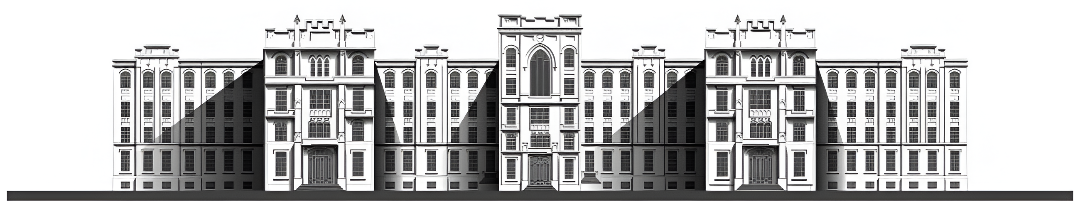
\includegraphics[width=\logowidth]{figuras/instituicao.png}\\
    }\par

    % Espaço vertical até a seção inferior
    \vfill

    % Seção inferior: local e data. Estas linhas aparecem junto à
    % margem inferior, respeitando a mesma fonte e alinhamento central.
    {\centering
      {\normalsize \local}\\
      {\normalsize \datadeposit}\\
    }\par
  }
\end{titlepage}
\clearpage
% Folha de rosto (contra‑capa) – inicia a contagem de páginas em algarismos árabes
% As folhas pré‑textuais são contadas a partir da folha de rosto.
\pagenumbering{arabic}
\setcounter{page}{1}
% ----------------------------------------------------------------------
% Folha de rosto (contracapa)
%
% A folha de rosto contém o nome da instituição, programa de
% pós‑graduação, título, autor, natureza do trabalho, nome(s) do
% orientador e coorientador, local e data. Esta folha é contada mas
% não numerada.

\begin{titlepage}
  % A folha de rosto é contada mas não numerada. 
  % estilo `pretext` para suprimir cabeçalho, rodapé e qualquer
  % espaçamento extra, garantindo que o texto comece imediatamente
  % após a margem superior.
  \thispagestyle{pretext}
  % Todo o texto da folha de rosto (exceto o bloco à direita) deve
  % aparecer em negrito. 
  {\bfseries
    % Nome do autor e título centralizados
    \begin{center}
      \vspace*{2cm}
      {\normalsize \autor}\\[1.5cm]
      % O título pode ocupar mais de uma linha; \setstretch{1.5} aplicado
      % para que a entrelinha do título acompanhe o espaçamento do texto
      % principal.
      {\normalsize\begingroup\setstretch{1.5}\titulo\par\endgroup}
      \vspace{2cm}
      %{\normalsize Versão original}\\[1.5cm]
    \end{center}
    % Informações sobre o programa e orientações. De acordo com as
    % diretrizes USP, esses dados devem ser alinhados a partir da metade
    % da parte impressa da página para a margem direita.
    % Para posicionar o bloco no meio da página, inserido um
    % deslocamento horizontal de metade da largura do texto (\textwidth)
    % utilizado \parbox com largura igual a metade da largura do
    % texto. O conteúdo da \parbox permanece à esquerda dentro desse
    % bloco, de forma que o texto inicie exatamente no meio da página.
    \noindent\hspace*{0.5\textwidth}%
    \parbox{0.5\textwidth}{%
      \normalfont % o bloco à direita não deve estar em negrito
      Dissertação apresentada à \instituicao\,\
      para avaliação no exame de qualificação do programa de pós-graduação\\[0.2cm]
      Programa de Obstetrícia e Ginecologia\\[0.2cm]
      Orientador(a): \orientador\
      \ifx\coorientador\undefined\else\\Coorientador(a): \coorientador\fi
    }
    \vfill
    \begin{center}
      {\normalsize \local}\\[0.2cm]
      {\normalsize \datadeposit}
    \end{center}
  }
\end{titlepage}

% As listas e resumos são elementos não numerados; centralizamos
% seus títulos conforme as diretrizes. A contagem de páginas segue
% sequencialmente, porém a numeração visível somente começará na Introdução.

% Resumo em português
\clearpage
\phantomsection
% ----------------------------------------------------------------------
% Resumo em Português
%
% Este arquivo contém o resumo do trabalho em português. O título
% “Resumo” deve ser centralizado e não numerado. A
% primeira linha do texto do resumo deve iniciar logo abaixo do título
% sem recuo. Usar espaço simples neste trecho conforme as normas.

% O título do resumo aparece centralizado, com mesma fonte das listas, e não é
% incluído no sumário.
{\centering
\large\bfseries Resumo\par}
% Insere 1,5cm de espaço vertical entre o título e o texto do resumo【543391667091976†L423-L441】.
\vspace{1.5cm}

% O resumo deve ser digitado em espaço simples.  Usa-se o
% ambiente singlespace fornecido pelo pacote setspace para aplicar
% espaçamento simples apenas nesta seção.
\begin{singlespace}
A duração gestacional termina em dois eventos mutuamente exclusivos, óbito
fetal e nascimento vivo, que frequentemente são analisados separadamente
apesar de sua natureza competitiva. Esta dissertação avaliou o tempo até o
parto no estado de São Paulo, combinando métodos de riscos competitivos com
uma estrutura bayesiana de fragilidade espacial compartilhada no nível das
Redes Regionais de Atenção à Saúde (RRAS). Foram utilizados microdados
públicos de 2023 do SIM-DOFET e do SINASC, harmonizados e analisados após
filtragem por casos completos, resultando em 3.266 óbitos fetais e 485.922
nascimentos vivos. As análises descritivas e as funções de incidência
acumulada mostraram forte assimetria entre os desfechos: os óbitos fetais se
concentraram em idades gestacionais mais precoces, enquanto os nascimentos
vivos se concentraram próximo ao termo. As CIF estratificadas indicaram
padrões sociais e obstétricos relevantes, incluindo perfis menos favoráveis
nos estratos de menor escolaridade materna e em grupos com histórico
obstétrico desfavorável. Os indicadores por RRAS revelaram heterogeneidade
territorial marcada, com descompasso entre carga absoluta e indicadores
relativos, sustentando a modelagem explícita da vulnerabilidade regional
latente. O modelo
bayesiano proposto de riscos competitivos com fragilidade ICAR foi desenvolvido
para fornecer estimativas regionais interpretáveis e com quantificação de
incerteza, apoiando o planejamento em saúde materna e perinatal no Sistema
Único de Saúde (SUS).


\vspace{0.5cm}
\noindent\textbf{Palavras‑chave:} óbito fetal. nascimento vivo. riscos
competitivos. fragilidade espacial. Redes Regionais de Atenção à Saúde.
\end{singlespace}

% Evita o cabeçalho na página do resumo
\thispagestyle{pretext}

% Abstract em inglês
\clearpage
\phantomsection
% ----------------------------------------------------------------------
% Abstract in English
%
% The abstract provides a concise summary of the research in English.

\selectlanguage{english}

{\centering
\large\bfseries Abstract\par}
% Insere 1,5 linhas de espaço entre o título e o texto do abstract,
% garantindo consistência com o espaçamento utilizado entre títulos
% e texto nas demais seções.
% Insere 1,5cm de espaço vertical entre o título e o texto do abstract.
\vspace{1.5cm}

% O abstract também deve ser digitado em espaço simples conforme as normas
% (citations, footnotes, references, captions etc.).
\begin{singlespace}
Gestational duration ends in two mutually exclusive events, stillbirth and
live birth, which are often analysed separately despite their competing nature.
This dissertation evaluated time to delivery in the state of Sao Paulo,
combining competing risks methods with a Bayesian shared spatial frailty
structure at the level of the Regional Health Care Networks (RRAS). Public
microdata from SIM-DOFET and SINASC for 2023 were harmonized and analysed
after complete-case filtering, resulting in 3,268 stillbirths and 485,922 live
births. Descriptive analyses and cumulative incidence functions showed a clear
asymmetry between outcomes: stillbirths were concentrated at earlier
gestational ages, whereas live births were concentrated near term. Stratified
CIFs indicated relevant social and obstetric patterns, including less favorable
profiles among lower maternal education groups and groups with unfavorable
obstetric history. Indicators by RRAS revealed marked territorial heterogeneity,
with divergence between absolute burden and rates, supporting explicit
modelling of latent regional vulnerability. The proposed Bayesian competing
risks model with ICAR frailty was developed to provide interpretable regional
estimates with uncertainty quantification, supporting maternal and perinatal
health planning within the Brazilian Unified Health System (SUS).

\vspace{0.5cm}
\noindent\textbf{Keywords:} stillbirth. live birth. competing risks. spatial
frailty. Regional Health Care Networks.
\end{singlespace}

% Retorna ao idioma principal (português) após o abstract.
\selectlanguage{brazilian}

% Evita o cabeçalho na página do abstract
\thispagestyle{pretext}

% Listas de figuras, tabelas e equações
% Segundo as diretrizes, as listas são elementos pré‑textuais opcionais
% apresentados após os resumos e antes do sumário.

% Renomeia "Lista de Figuras" para "Lista de Ilustrações"
\renewcommand{\listfigurename}{Lista de Ilustrações}

% Lista de ilustrações (figuras)
\clearpage
\phantomsection
\listoffigures
% Evita o cabeçalho na página da lista de figuras
\thispagestyle{pretext}

% Lista de tabelas
\clearpage
\phantomsection
\listoftables
% Evita o cabeçalho na página da lista de tabelas
\thispagestyle{pretext}

% Lista de equações
\clearpage
\phantomsection
\listofequations
% Evita o cabeçalho na página da lista de equações
\thispagestyle{pretext}

% Sumário (índice) – deve aparecer após os resumos e listas.
\clearpage
\phantomsection
\tableofcontents
% Evita o cabeçalho na página do sumário
\thispagestyle{pretext}


%------------------------------ Elementos textuais

% Antes da introdução, encerramos os elementos pré‑textuais. A
% numeração já foi iniciada na folha de rosto (contracapa) e
% incrementada nas páginas subsequentes. Para retornar os valores de
% \headheight e \headsep aos originais e ativar o estilo de
% cabeçalho com linha e numeração, restauramos esses comprimentos e
% definimos o estilo fancy.
\clearpage
\setlength{\headheight}{14.5pt}
\setlength{\headsep}{0.5cm}
\pagestyle{fancy}

% ----------------------------------------------------------------------
% Capítulo: Introdução
%
% A introdução é a primeira parte da estrutura textual e deve iniciar na
% página 1, com numeração em algarismos arábicos. Usar o comando
% \chapter para produzir o título numerado e siga as diretrizes de
% espaçamento e formatação. Os títulos de seções subsequentes devem
% respeitar a numeração progressiva.

\chapter{Introdução}

O estudo do tempo até o parto constitui um problema relevante na pesquisa em saúde 
perinatal, especialmente quando diferentes desfechos podem ocorrer ao longo da mesma 
escala temporal. Entre esses desfechos destacam-se o óbito fetal e o nascimento vivo, 
eventos terminais e mutuamente exclusivos que caracterizam a evolução temporal da 
gestação. Na epidemiologia aplicada, esses desfechos são frequentemente analisados 
em modelos separados, o que enfraquece a interpretação temporal e pode gerar 
inconsistências quando um evento impede a ocorrência do outro. O tempo gestacional, 
portanto, se ajusta a uma estrutura de riscos competitivos, na qual riscos 
causa-específicos e funções de incidência acumulada (CIF, do inglês 
\textit{Cumulative Incidence Function}) são mais apropriados do que métodos 
de sobrevivência de evento único \cite{satagopan2004note,finegray1999,
naimi2016cumulative,smith2016competing}.

Nesta dissertação, o interesse central é avaliar o tempo até o parto em
gestações de residentes no estado de São Paulo, considerando o óbito fetal e o
nascimento vivo como eventos competitivos. Essa abordagem permite tratar o nascimento 
vivo não apenas como um registro de encerramento da gestação, mas como um desfecho 
que impede a observação posterior do óbito fetal naquela mesma gestação. Ao mesmo 
tempo, a inclusão dos nascidos vivos aproxima o estudo de outro tema importante 
em obstetrícia, sendo este, o problema da prematuridade. Dessa forma, o trabalho 
não se restringe à mortalidade fetal, mas busca compreender a dinâmica temporal 
do parto em presença de desfechos competitivos. O estado de São Paulo, por sua vez, 
apresenta um cenário estratégico para análise devido à sua população numerosa e 
heterogênea, com grande volume de nascimentos, ampla rede hospitalar, desigualdades 
regionais, diferentes níveis de organização da rede assistencial, aspectos que 
podem ser parcialmente investigados (no âmbito deste estudo) por meio de dados 
públicos do Sistema de Informações sobre Nascidos Vivos (SINASC) e do Sistema de 
Informações sobre Mortalidade (SIM).

Além disso, é necessária atenção à definição dos casos, dado que diferentes critérios 
podem ser utilizados na caracterização dos desfechos, principalmente em relação ao 
óbito fetal, cujas definições podem variar entre sistemas nacionais e critérios 
internacionais de comparabilidade \cite{Andrade2005,Lawn2016}.

\section{Definição dos desfechos perinatais e cenário global}

No Brasil, a Declaração de Óbito deve ser emitida para óbito fetal quando a
gestação tiver duração igual ou superior a 20 semanas, ou quando o feto
apresentar peso corporal igual ou superior a $500\,\text{g}$, ou estatura igual
ou superior a $25\,\text{cm}$ \cite{ministerioSaudeDO2022}. Este é o critério
que orienta a definição adotada neste estudo e também é compatível com a
normatização nacional para emissão da Declaração de Óbito \cite{Andrade2005}. O 
nascimento vivo, por sua vez, é definido como a expulsão ou extração completa 
do produto da concepção que, após a separação do corpo materno, apresenta 
respiração ou qualquer outro sinal de vida, independentemente da duração da 
gestação \cite{ministerioSaudeDNV2022}. Portanto, mesmo nas idades gestacionais 
mais precoces, um recém-nascido com sinais de vida é registrado como nascido 
vivo. Essas definições são importantes para compreensão dos desfechos perinatais 
ao longo da gestação e consistência das informações apresentadas.

Em ambas definições, a idade gestacional é de extrema importância, pois a interpretação 
clínica e epidemiológica dos desfechos depende do momento gestacional em que o parto 
ocorre. A prematuridade entra nesse raciocínio por estar contida no conjunto dos
nascidos vivos. A Organização Mundial da Saúde (OMS) define nascimento prematuro
como aquele ocorrido antes de 37 semanas completas de gestação, tendo como subdivisões 
a prematuridade extrema, muito prematuro e prematuridade moderada a tardia
\cite{WHO2023Preterm}. Estimativas globais de 2020 indicaram a ocorrência de 13,4 
milhões de nascimentos prematuros, com importante variação entre países e
regiões \cite{Ohuma2023PretermEstimates}. O relatório \textit{Born Too Soon},
publicado pela OMS, Fundo das Nações Unidas para a Infância (UNICEF) e
parceiros, reforçou que a carga da prematuridade permanece elevada, com pouco
avanço global na última década e forte relação com desigualdades no acesso e na
qualidade do cuidado materno e neonatal \cite{BornTooSoon2023}. De forma semelhante, 
estimativas internacionais recentes mostram que a carga de óbito fetal permanece 
elevada e distribuída de modo desigual entre países e sistemas de saúde \cite{Lawn2016,UnitedNationsChildMortality,Neglectedt}. 
Esses elementos reforçam a importância de analisar não apenas a ocorrência dos desfechos, 
mas também o momento gestacional em que eles acontecem e o contexto assistencial 
em que a gestação foi acompanhada.

Diante da elevada carga global de prematuridade e óbito fetal, bem como das 
desigualdades observadas, torna-se importante compreender o panorama brasileiro 
considerando os desfechos perinatais em questão.

\section{Panorama brasileiro}

No Brasil, a mortalidade fetal e a prematuridade seguem sendo importantes problemas 
de saúde perinatal, fortemente relacionados às condições de saúde materna, à qualidade 
do cuidado pré-natal e à assistência ao parto. Em estudo nacional recente com dados do 
Sistema de Informações sobre Mortalidade (SIM), considerando óbitos fetais com idade 
gestacional igual ou superior a 20 semanas, Rocha et al. observaram que esses óbitos 
representaram 1,14\% dos nascimentos ocorridos no período de 1996 a 2021, com taxa 
global (considerando todo o período) de 11,4 óbitos fetais por 1.000 nascimentos 
\cite{rocha2025space}. Apesar de Rocha et al. observarem uma redução de aproximadamente 
20\% na taxa de mortalidade fetal nesse período, a queda não foi homogênea no território 
nacional, sendo observadas maiores taxas e reduções mais lentas nas regiões Norte, 
Nordeste e Centro-Oeste, evidenciando desigualdades regionais \cite{rocha2025space}. 
Além disso, cerca de 93\% dos óbitos ocorreram antes do parto, aspecto que reforça a 
relevância da vigilância durante a gestação.

Esse padrão de desigualdade também aparece quando se observa o nascimento vivo pela 
perspectiva da prematuridade. Análises nacionais baseadas no Sistema de Informações 
sobre Nascidos Vivos (SINASC), envolvendo mais de 25,5 milhões de nascidos vivos 
entre 2014 e 2023, indicaram aumento da prevalência de prematuridade de 11,3\% em 
2014 para 11,9\% em 2023 \cite{Victor2025PretermBrazil}. As maiores prevalências 
foram observadas entre mães com 35 anos ou mais, mães com menos de 20 anos, mulheres 
sem escolaridade formal e nas regiões Norte e Nordeste \cite{Victor2025PretermBrazil}. 
Esse padrão é coerente com o Boletim Epidemiológico do Ministério da Saúde sobre 
nascimentos prematuros no período de 2012 a 2022, que descreve a prematuridade 
como evento associado a fatores sociodemográficos, condições maternas, cuidado 
pré-natal e características da gestação \cite{BrasilBoletimPrematuridade2024}. 
Além disso, o Brasil registrou 2.537.511 nascidos vivos em 2023, dos quais 304.501 foram 
prematuros, correspondendo a 12\% do total \cite{OOBrPainelVigilancia}. 
Esses números ajudam a dimensionar a magnitude da prematuridade no país e reforçam 
a relevância epidemiológica dos desfechos perinatais no contexto brasileiro.

Essas evidências indicam que os desfechos perinatais em questão apresentam importante 
variabilidade em território nacional, mostrando a importância de análises que considerem 
diferenças regionais e contextos assistenciais específicos. Assim, o estado de São Paulo 
apresenta um cenário de grande interesse de investigação dado o elevado volume de 
nascimentos e à complexidade de sua organização regional de saúde. 

\section{Contexto do estado de São Paulo e das RRAS}

O recorte do estado de São Paulo, embora sendo parte desse cenário nacional,
acrescenta uma dimensão própria. O estado reúne grande volume de nascimentos e 
uma rede assistencial complexa, com diferenças internas de organização, capacidade 
instalada e fluxos regionais de atenção. A regionalização da saúde no estado é 
organizada, dentre outras, por Regiões de Saúde e Redes Regionais de Atenção à 
Saúde (RRAS), estruturas voltadas à integração de ações e serviços no território 
\cite{SESSPRegionalizacao2026}. Para a análise de dados de 2023, essa organização 
regional é importante porque permite avaliar se o risco de óbito fetal e a distribuição 
do nascimento vivo variam entre agregados territoriais que compartilham redes de 
referência e condições assistenciais semelhantes.

Em 2023 o estado de São paulo registrou 503.903 nascidos vivos, do quais 60.468 foram 
prematuros, o que corresponde a aproximadamente 12\% do total \cite{OOBrPainelVigilancia}. 
Esses valores situam o estado dentro do cenário nacional de prematuridade e reforçam 
a importância de estudar o tempo até o parto em uma população numerosa, em linha 
com estudos nacionais que descrevem a prematuridade como evento frequente e 
socialmente distribuído no Brasil \cite{Victor2025PretermBrazil,BrasilBoletimPrematuridade2024}. 
Entretanto, para os óbitos fetais, a contextualização estadual exige cautela adicional, 
pois as estimativas disponíveis podem variar conforme a definição adotada para o 
desfecho, especialmente em relação à idade gestacional mínima considerada. Dados 
disponíveis e estudos recentes conduzidos nesse recorte adotaram definições mais 
restritivas, como óbitos a partir de 22 semanas de gestação. Assim, a magnitude 
estadual do óbito fetal será apresentada diretamente nas análises do estudo, de 
acordo com a definição adotada para a construção da população analisada. 

A necessidade de considerar heterogeneidade territorial também é sustentada pela
literatura. No município de São Paulo, um estudo identificou diferenças
intraurbanas de mortalidade fetal segundo agrupamentos de vulnerabilidade
social, indicando que a distribuição dos óbitos não se resume ao volume
populacional das áreas analisadas \cite{Marques2021FetalSocialVulnerabilitySP}.
Além disso, o estudo FetRiskS, realizado em hospitais públicos do município de
São Paulo com dados coletados entre 2019 e 2023, descreveu o óbito fetal como
evento relacionado a fatores socioeconômicos, acesso inadequado ao pré-natal,
condições maternas, alterações placentárias, restrição de crescimento fetal e
malformações congênitas \cite{Marques2026FetRiskS}. Embora esses achados não possam 
ser refletidos para o conjunto estadual e das RRAS, eles apontam para a importância 
de considerar que a região de residência possa aproximar condições contextuais 
compartilhadas relacionadas à organização da rede, ao acesso aos serviços e às 
condições de assistência durante a gestação e o parto.

Assim, o estado de São Paulo não foi escolhido apenas pelo tamanho da base de 
dados, mas também por reunir regiões com diferentes formas de organização da 
rede de saúde, capacidade assitencial e condições de acesso ao cuidado. Este cenário 
é adequado para investigar se o risco e a dinâmica temporal do óbito fetal e do nascimento 
vivo varia entre regiões, mesmo após considerar as características maternas, fetais, 
obstétricas e assistenciais disponíveis no SIM-DOFET e no SINASC. Caso a região 
de residência permaneça associada aos riscos estimados após o ajuste, esse resultado 
não deve ser interpretado como prova de que a região, por si só, determine o 
desfecho. De forma mais cautelosa, essa associação deve ser vista como possível 
indicativo de diferenças contextuais não captadas pelas variáveis individuais 
disponíveis, reforçando a importância de considerar, em conjunto, fatores maternos, 
fetais, obstétricos, assistenciais e territoriais associados aos desfechos 
gestacionais.

\section{Fatores associados aos desfechos gestacionais}

A interpretação dos desfechos gestacionais requer considerar o caráter multifatorial 
desses eventos. Tanto o óbito fetal quanto a prematuridade resultam da interação 
entre fatores maternos, fetais, placentários, obstétricos, assistenciais e sociais 
que atuam de forma simultânea e, muitas vezes, dependente ao longo da gestação. 
Documentos clínicos e revisões da literatura apontam de forma recorrente a associação 
de óbito fetal com condições como hipertensão crônica, pré-eclâmpsia, diabetes, 
obesidade, tabagismo, idade materna avançada, gestação múltipla, histórico obstétrico 
desfavorável e vulnerabilidade social \cite{Lawn2016,ACOG2020Stillbirth,Sun2018,zile2019maternal}. 
De maneira similar, a prematuridade compartilha parte importante desses fatores, embora 
seja registrada entre os nascidos vivos. Estudos observacionais e revisões da literatura 
descrevem o nascimento prematuro como um desfecho associado a diferentes condições 
maternas, históricas, obstétricas, ambientais e socioeconômicas, frequentemente 
relacionadas ao longo da gestação \cite{Mitrogiannis2023PretermRisk}. No Brasil, 
evidências recentes mostram maior frequência de prematuridade nos extremos de idade 
materna, em contextos de menor escolaridade, em gestações de maior complexidade e em 
grupos com menor acesso a cuidado pré-natal adequado 
\cite{Victor2025PretermBrazil,BrasilBoletimPrematuridade2024}. Assim, fatores como 
baixa escolaridade, vulnerabilidade socioeconômica e acesso limitado ao pré-natal 
não devem ser interpretados apenas como características individuais, mas também 
como marcadores de trajetórias sociais e assistenciais distintas durante a gestação.

Entre os fatores fetais e placentários, destacam-se restrição de crescimento
fetal, malformações congênitas, anomalias genéticas, insuficiência placentária e
descolamento prematuro de placenta \cite{gardosi2013maternal,smith2007stillbirth,pinar2014placental}. 
A restrição de crescimento fetal é particularmente importante porque pode permanecer 
não identificada durante o pré-natal e se manifestar apenas no desfecho da gestação. 
Além disso, muitos desses fatores atuam de forma dependente. A obesidade e a diabetes, 
por exemplo, podem aumentar o risco de distúrbios hipertensivos, enquanto distúrbios 
hipertensivos podem comprometer a função placentária e favorecer insuficiência 
placentária que, por sua vez, pode antecipar o parto ou resultar em óbito fetal. Essa 
dependência reforça a importância de analisar simultaneamente o óbito fetal e o 
nascimento vivo ao longo da gestação, visto que certas características podem estar 
associadas tanto ao risco de óbito intrauterino quanto ao momento gestacional em 
que o parto ocorre.

As variáveis disponíveis no SIM-DOFET e no SINASC permitem representar apenas parte
desse conjunto de fatores descritos na literatura. Idade materna, escolaridade, 
raça/cor, tipo de gestação, histórico reprodutivo, número de filhos vivos 
e mortos previamente, consultas de pré-natal e momento de início do pré-natal 
representam características maternas, sociais, obstétricas e assistenciais frequentemente 
associadas aos desfechos gestacionais \cite{Victor2025PretermBrazil,Marques2026FetRiskS,
ACOG2020Stillbirth,Silva2026PrenatalInequities}. Da mesma forma, peso ao nascer ou 
peso fetal, sexo, presença de anomalia e Apgar no quinto minuto, quando disponível, 
representam características fetais e neonatais relevantes, embora algumas delas 
sejam medidas no momento do desfecho e, portanto, devam ser interpretadas como 
marcadores do processo gestacional ou do estado ao nascimento, e não necessariamente 
como causas antecedentes. De maneira similar, variáveis como tipo de parto, local 
de ocorrência, indução do trabalho de parto e cesariana antes do início do trabalho 
de parto refletem decisões e condições assistenciais próximas ao encerramento da 
gestação, o que exige cautela na interpretação. 

Embora o SIM-DOFET e o SINASC registrem informações essenciais sobre a mãe, a 
gestação, o feto, o nascimento e o óbito, essas bases representam apenas parte 
dos processos clínicos, assistenciais e sociais envolvidos nos desfechos 
gestacionais. O cuidado pré-natal é um exemplo dessa limitação. Embora seja uma 
fator importante da assistência durante a gestação, sua interpretação no 
SINASC exige cautela, pois a base informa principalmente o número de consultas 
registradas, e não a qualidade clínica do acompanhamento prestado. Em estudo 
nacional com dados de 2023, Silva et al. observaram que a realização de ao 
menos uma consulta de pré-natal apresentava cobertura considerável entre os 
nascidos vivos, mas que apenas 67,4\% dos registros indicavam oito ou mais 
consultas \cite{Silva2026PrenatalInequities}. Esse contraste sugere que a 
cobertura inicial do pré-natal é elevada no país, embora o acompanhamento mais 
completo ainda apresente desigualdades por escolaridade materna, raça/cor, 
idade e região.

Além do pré-natal, outros aspectos relevantes do acompanhamento gestacional e da 
assistência ao parto não estão disponíveis de forma completa e padronizada nas 
bases utilizadas, como resultados de exames, condutas clínicas adotadas durante 
a gestação e o parto e condições socioeconômicas individuais mais detalhadas. 
Mesmo variáveis de alta relevância para este estudo, como a idade 
gestacional, podem apresentar limitações de concordância e diferenças regionais 
de mensuração, apesar da elevada cobertura nacional do SINASC 
\cite{Szwarcwald2019SINASC}. Por isso, os resultados devem ser interpretados 
como associações estimadas a partir de registros populacionais, e não como uma 
evidência direta dos mecanismos clínicos responsáveis por cada desfecho. Esse 
conjunto de limitações reforça a importância de abordagens metodológicas capazes 
de considerar simultaneamente múltiplos fatores associados, restrições derivadas 
das bases de dados e possíveis diferenças contextuais entre regiões.

\section{Relevância metodológica}

A análise de sobrevivência é adequada para este problema porque a idade gestacional 
representa o tempo até a ocorrência do desfecho. Entretanto, quando o interesse 
envolve óbito fetal, o nascimento vivo não deve ser tratado como censura. Ao ocorrer 
o nascimento vivo, a gestação se encerra e o óbito fetal deixa de ser possível. 
Desconsiderar essa estrutura pode distorcer a interpretação do risco acumulado ao 
longo da gestação, especialmente em idades gestacionais nas quais os nascimentos 
vivos se tornam cada vez mais frequentes \cite{naimi2016cumulative,smith2016competing}. 
Os modelos de riscos competitivos oferecem uma forma mais coerente de lidar com isso, 
pois reconhecem que diferentes desfechos competem pelo encerramento do tempo de 
seguimento \cite{satagopan2004note,finegray1999,naimi2016cumulative,Austin2016CompetingRisks}. 

Além da presença de riscos competitivos, os dados possuem uma estrutura regional 
formada pelas RRAS, de forma que gestantes residentes em uma mesma RRAS estão 
inseridas em um mesmo contexto territorial e assistencial, podendo compartilhar 
condições semelhantes de acesso aos serviços, disponibilidade de recursos de saúde 
e características socioambientais não mensuradas pelas variáveis disponíveis. Essa 
interpretação é coerente com a organização regional da assistência em saúde e com 
evidências de desigualdades territoriais em desfechos perinatais 
\cite{rocha2025space,SESSPRegionalizacao2026,Marques2021FetalSocialVulnerabilitySP}. 
Nesse contexto, modelos com fragilidade compartilhada permitem incorporar a 
dependência entre observações pertencentes a uma mesma RRAS por meio de efeitos 
aleatórios associados às unidades regionais. Esses efeitos representam fontes de 
heterogeneidade não observada e acomodam a correlação intra-regional 
\cite{clayton1978model,vaupel1979impact,balan2020tutorial}. Quando essa 
heterogeneidade apresenta estrutura territorial, prioris espaciais do tipo ICAR 
permitem que regiões vizinhas compartilhem informação durante a estimação 
\cite{besag1991,rueheld2005}. Assim, após o ajuste pelas covariáveis medidas, a 
presença de variação residual entre RRAS pode indicar que diferenças regionais 
não captadas individualmente ou outros fatores não considerados ainda influenciam 
o risco dos desfechos analisados.

Essa estrutura metodológica é coerente com o principal problema do estudo: analisar 
o tempo até o parto, considerando que óbito fetal e nascimento vivo são eventos 
competitivos e que os dados estão organizados em um território regionalizado. A 
contribuição esperada não é apenas estimar associações individuais, mas oferecer uma 
forma de análise que respeite a natureza dos desfechos perinatais e a organização 
territorial da assistência em saúde. 

Os capítulos seguintes desenvolvem essas ideias de forma mais detalhada. O Capítulo 2 
apresenta os objetivos gerais e específicos do estudo. O Capítulo 3 descreve as 
fontes de dados, o processo de construção das bases, as variáveis utilizadas e a 
fundamentação estatística do modelo. O Capítulo 4 reúne os resultados das análises 
descritivas e dos modelos ajustados.

\chapter{Objetivos}

Avaliar o tempo até o parto em gestações de residentes no estado de São Paulo no 
ano de 2023, considerando óbito fetal e nascimento vivo como desfechos 
competitivos, e investigar a associação de características maternas, fetais, 
obstétricas, assistenciais e regionais com a distribuição desses desfechos ao 
longo da idade gestacional, com incorporação da possível heterogeneidade entre as 
Redes Regionais de Atenção à Saúde (RRAS).

\section{Objetivos específicos}

\begin{enumerate}
    \item Descrever os dados por meio de métodos de análise descritiva e de 
    sobrevivência, a fim de caracterizar o perfil das gestações e dos desfechos 
    perinatais registrados no SINASC e no SIM-DOFET, no estado de São Paulo em 2023.

    \item Desenvolver e ajustar um modelo paramétrico bayesiano de riscos competitivos 
    com fragilidade espacial compartilhada por RRAS, de forma a estimar associações 
    com os desfechos e representar heterogeneidade regional não observada.
\end{enumerate}
% ----------------------------------------------------------------------
% Capítulo: Materiais e Métodos
%
% Neste capítulo descrevem‑se os dados, a metodologia estatística e os
% procedimentos analíticos utilizados. Segue as normas de numeração
% progressiva das seções e subseções.

\chapter{Material e métodos}
\section{Fontes e coleta de dados}

Todo o desenvolvimento computacional deste estudo foi realizado utilizando o 
software R (versão 4.5.1)\cite{rsoftware}. Além disso, os dados de interesse 
foram extraídos por meio do pacote \texttt{microdatasus}\cite{saldanha2019microdatasus}. 
A seguir, são detalhadas as bases de dados utilizadas e os procedimentos metodológicos 
adotados.

\subsection{Sistema de Informações sobre Mortalidade - Declaração de Óbitos
Fetais (SIM-DOFET)}

Os dados públicos de mortalidade no Brasil são disponibilizados pelo Sistema de 
Informações sobre Mortalidade (SIM) \cite{DATASUSSIM2023}. Especificamente, os óbitos fetais são 
registrados em uma extensão do SIM para declarações de óbitos fetais 
(SIM-DOFET), no qual os casos são incluídos de acordo com critérios padronizados 
pelo Ministério da Saúde. De forma geral, óbito fetal é definido como a morte do 
produto da concepção antes da expulsão ou extração completa do corpo materno, 
independentemente da duração da gestação, na ausência de qualquer sinal de vida 
após a separação, como respiração, batimentos cardíacos, pulsações do cordão 
umbilical ou movimentos musculares voluntários efetivos \cite{Andrade2005,Lawn2016}. 
No Brasil, recomenda-se o preenchimento da Declaração de Óbito Fetal para perdas 
gestacionais com idade gestacional igual ou superior a 20 semanas, peso fetal igual 
ou superior a 500 gramas ou estatura igual ou superior a 25 centímetros \cite{Andrade2005,ministerioSaudeDO2022}. 
Entretanto, como a base do SIM-DOFET utilizada neste estudo não dispõe de informação 
sobre a estatura, a definição adotada considera como óbito fetal os registros que 
atenderam aos critérios para idade gestacional e peso fetal definidos.

A Figura \ref{fig:fluxograma-sim} apresenta o fluxograma do processo de seleção
dos registros até a obtenção da base de óbitos fetais no ano de 2023, no estado
de São Paulo e sem dados faltantes nas variáveis de interesse, totalizando 3.266
óbitos fetais para análise.

%------------------------ Fluxograma SIM-DOFET
\begin{figure}[H]
  \centering
  \caption{Fluxograma das etapas de filtragem e obtenção dos dados de óbitos
  fetais utilizados no estudo.}
  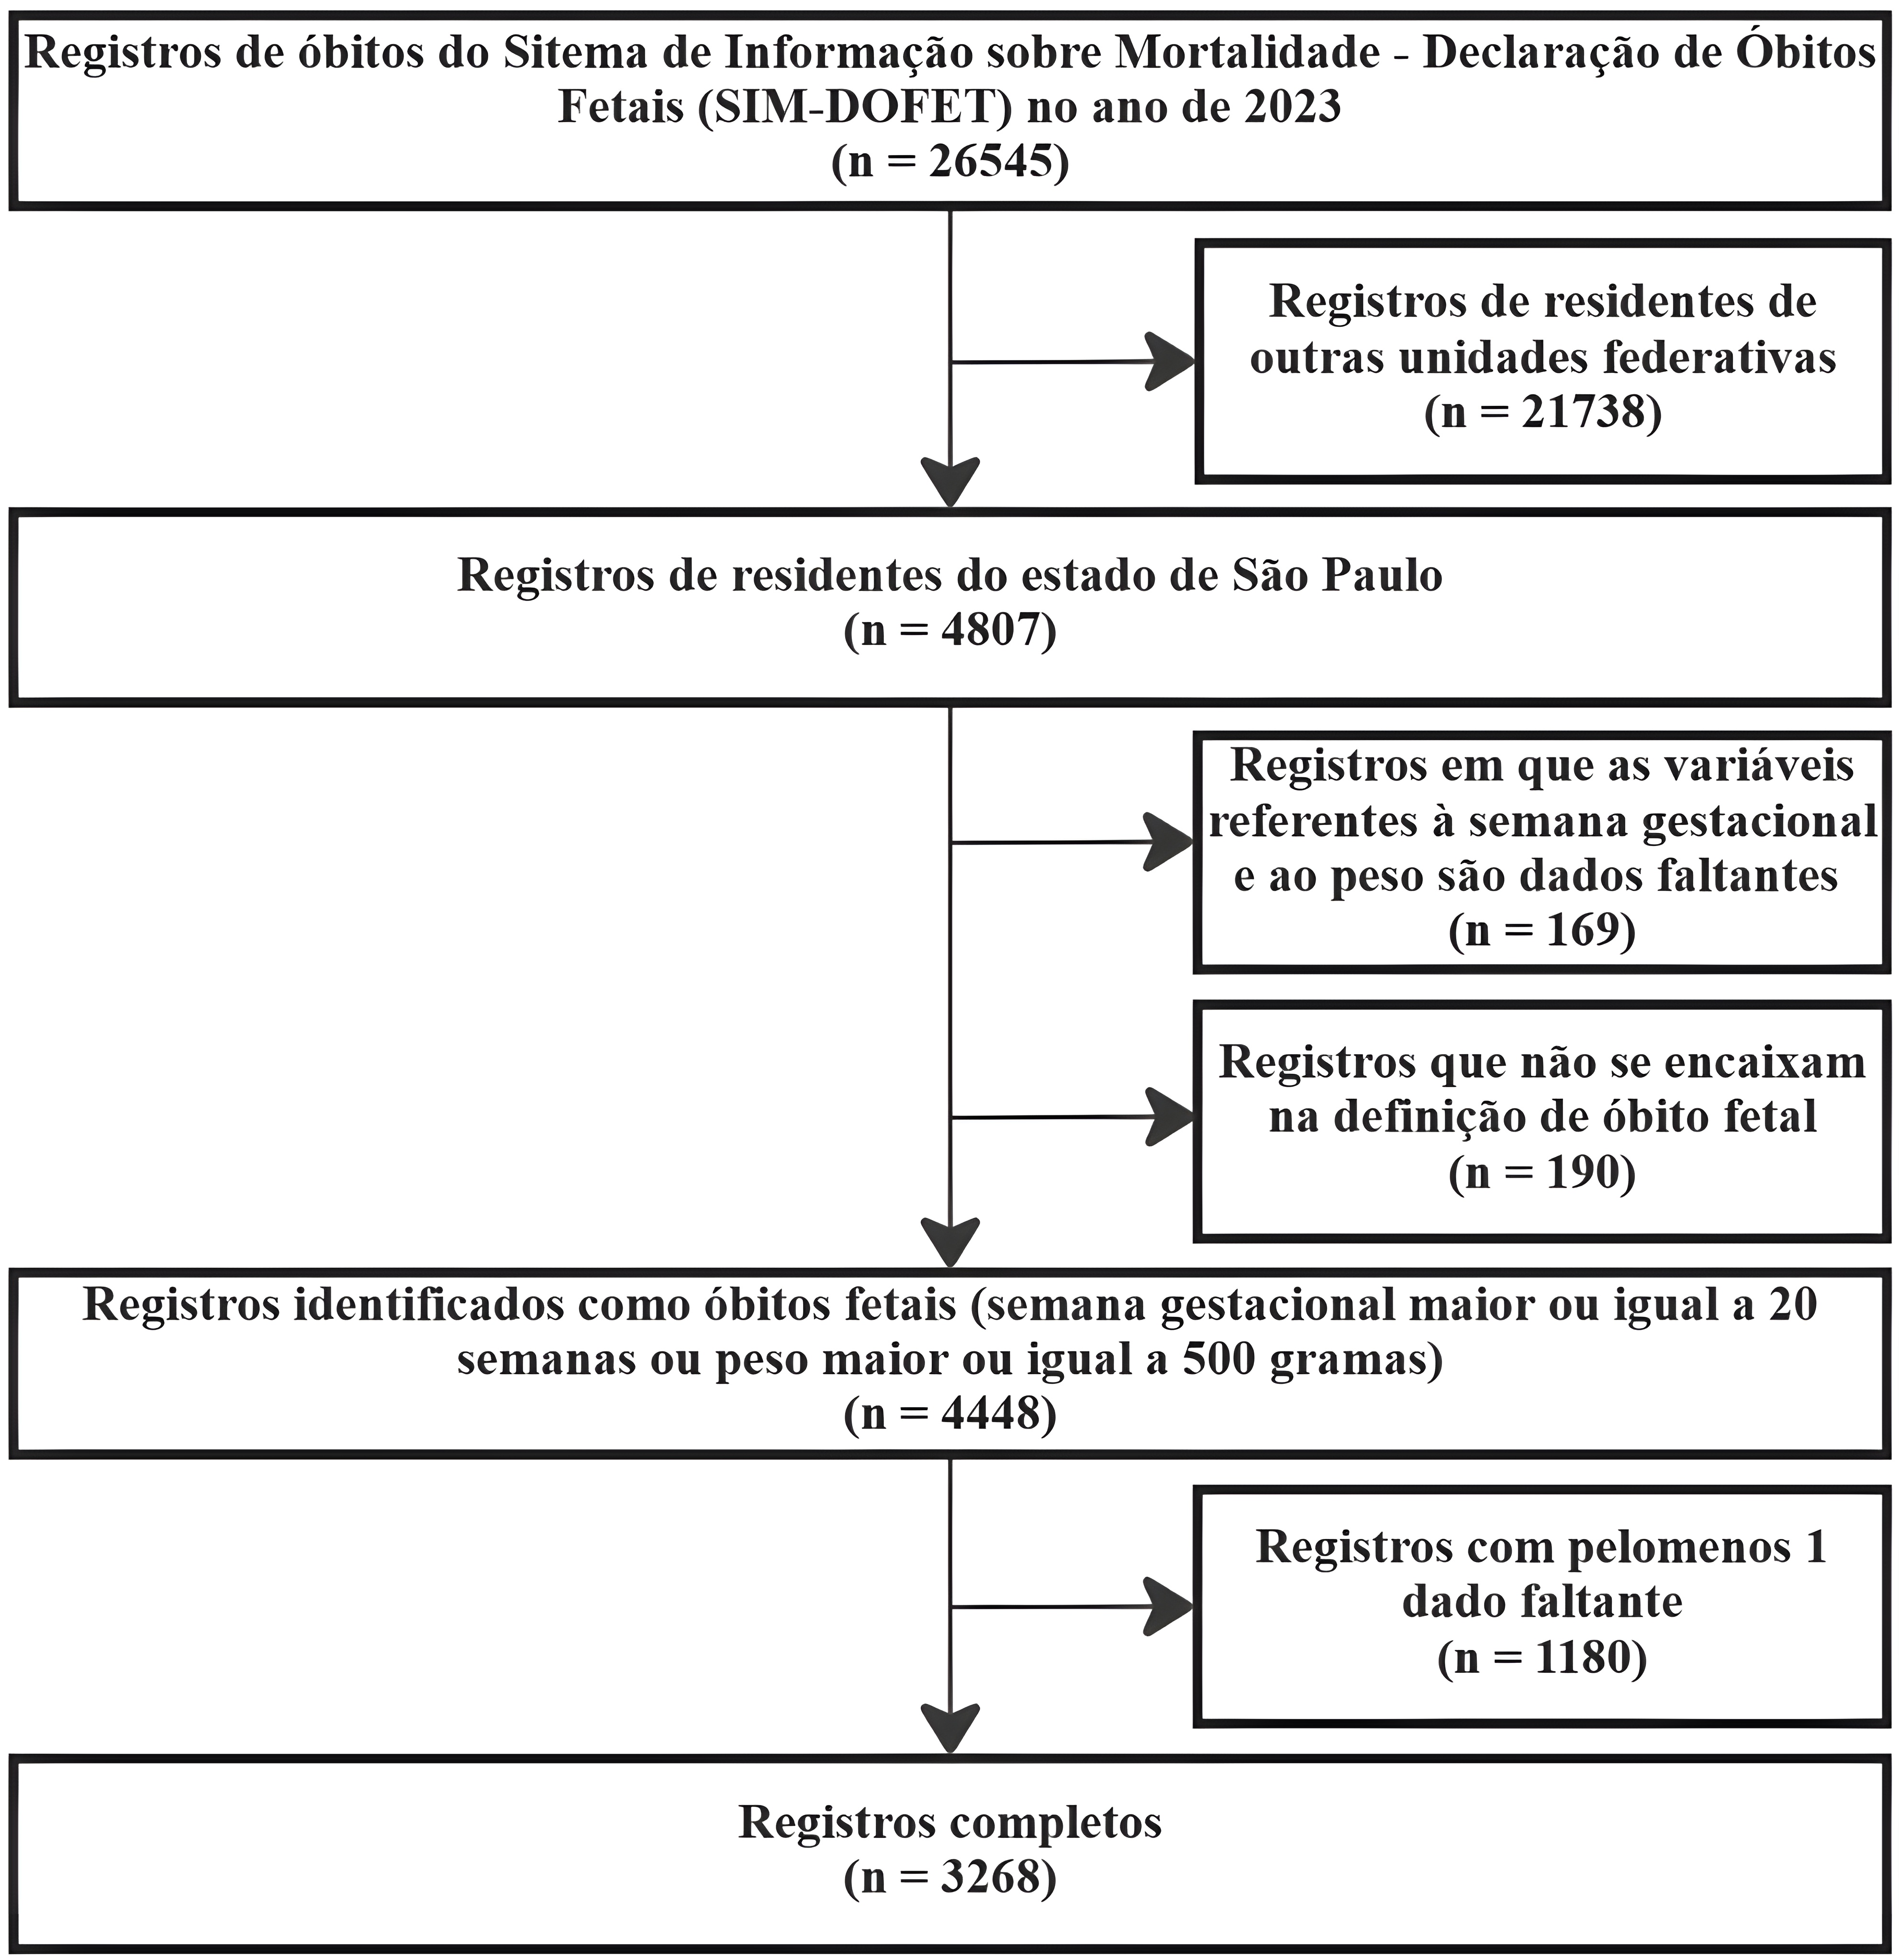
\includegraphics[width=0.8\linewidth]{figuras/flux_obitos_fetais.png}
  \fonte{Fonte: figura elaborada pelo autor.}
  \label{fig:fluxograma-sim}
\end{figure}

%------------------------ Fluxograma SINASC
\subsection{Sistema de
Informações sobre Nascidos Vivos (SINASC)}

Os dados de nascidos vivos são disponibilizados por meio do Sistema de
Informações sobre Nascidos Vivos (SINASC) \cite{DATASUSSINASC2023}, o qual é alimentado pela Declaração de 
Nascido Vivo (DNV). Para fins de registro, nascimento vivo é definido como a 
expulsão ou extração completa do produto da concepção do corpo materno que, 
após a separação, apresenta respiração ou qualquer outro sinal de vida, como 
batimentos cardíacos, pulsação do cordão umbilical ou movimentos musculares 
voluntários, independentemente da duração da gestação \cite{ministerioSaudeDNV2022}. 
No contexto deste estudo, em que o interesse é o tempo até o parto, gestações que
resultam em nascimento vivo do feto são caracterizadas como evento competidor 
\cite{satagopan2004note,naimi2016cumulative}. Isso ocorre porque, uma vez 
desencadeado o óbito fetal, torna-se impossibilitada a ocorrência de nascimento 
vivo. De forma análoga, se o desfecho observado primeiro é o nascimento vivo, o 
óbito fetal passa a ser impossibilitado, independentemente do tempo de observação 
do caso.

A Figura \ref{fig:fluxograma-sinasc} apresenta o fluxograma das etapas de processamento 
da base de dados, considerando os registros de 2023 para o estado de São Paulo e 
sem dados faltantes nas variáveis de interesse, totalizando 485.922 nascimentos 
vivos válidos.

\begin{figure}[H]
  \centering
  \caption{Fluxograma das etapas de filtragem e obtenção dos dados de nascidos
  vivos utilizados no estudo.}
  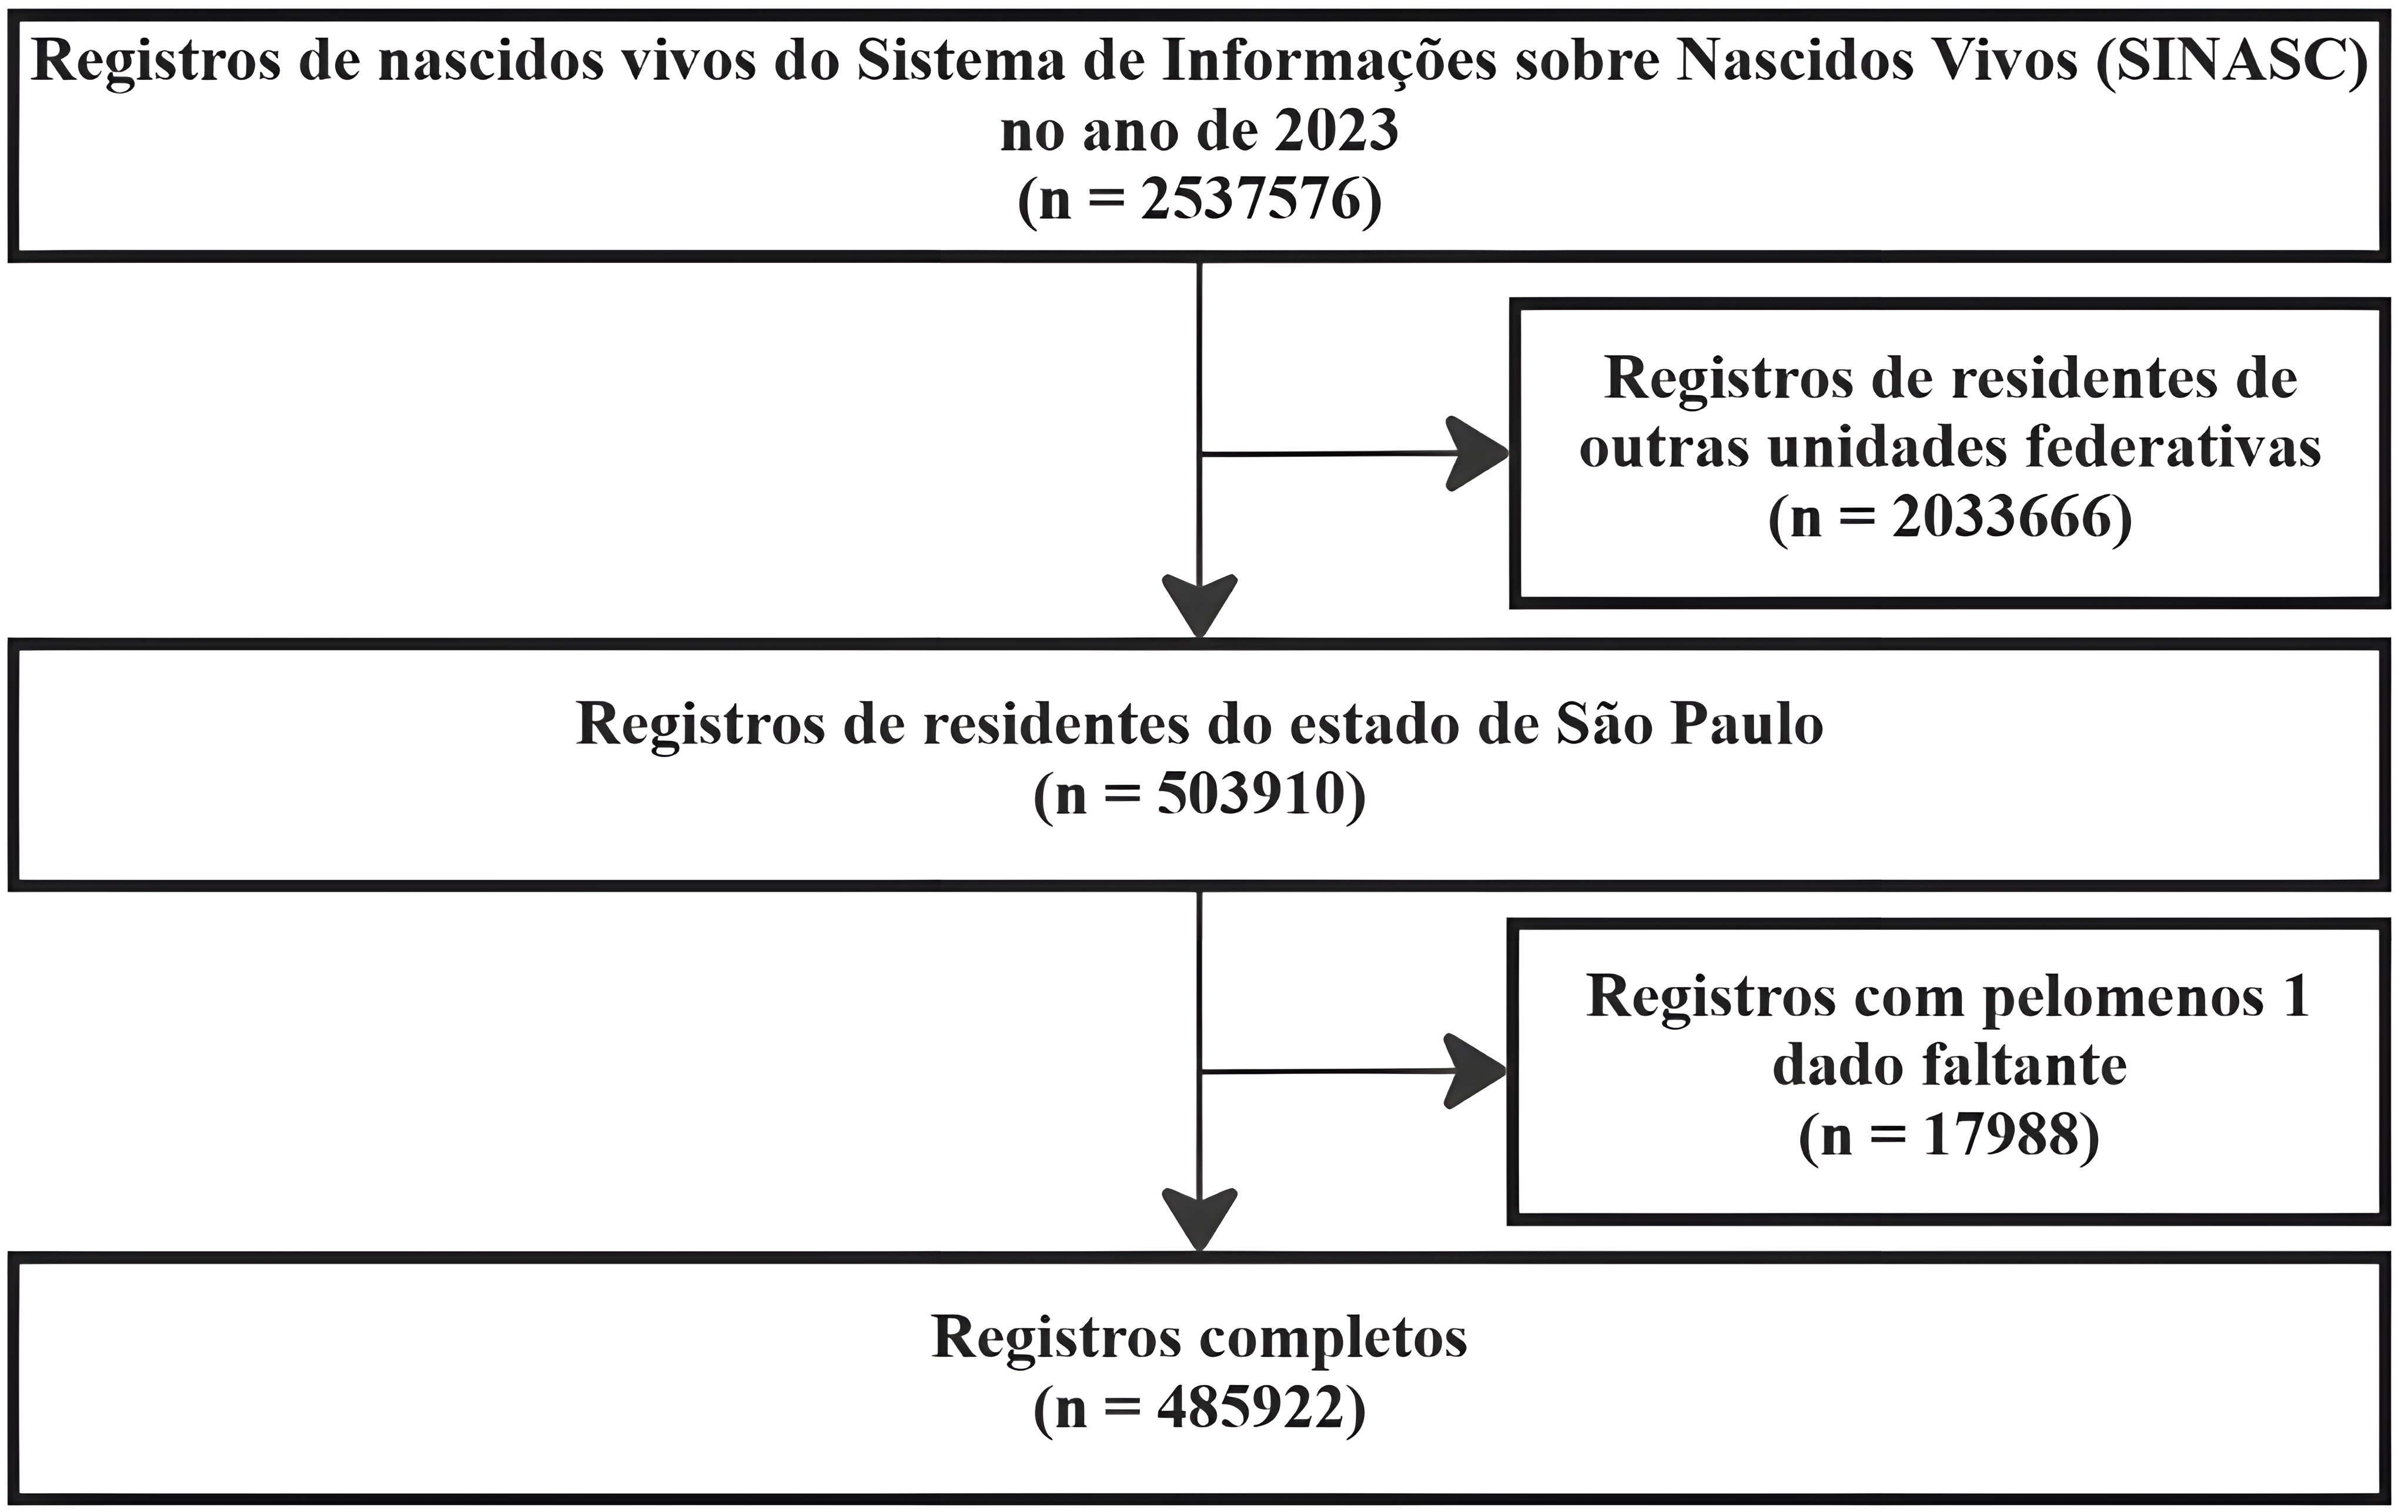
\includegraphics[width=0.8\linewidth]{figuras/flux_nascidos_vivos.png}
  \fonte{Fonte: figura elaborada pelo autor.}
  \label{fig:fluxograma-sinasc}
\end{figure}

\subsection{Variáveis abordadas e dados faltantes}

Foram inicialmente selecionadas 23 variáveis das bases de dados sendo consideradas, 
sendo 11 exclusivas do SINASC, 1 exclusiva do SIM-DOFET e 11 variáveis existentes em 
ambas. Além dessas, foi construída uma variável regional referente à RRAS de residência, 
obtida a partir do município de residência da mãe. As descrições das variáveis são 
apresentadas na Tabela \ref{fig:tabela-variaveis}.

%------------------------ Tabela com a lista das variáveis
\begin{table}[H]
    \centering
    \caption{Lista das variáveis abordadas no estudo.}
    \label{tab:variables}
    
    \small
    \renewcommand{\arraystretch}{1.05}
    \begin{tabular}{@{} L{3cm} L{7cm} L{3cm} @{}} 
        % Linha superior mais espessa
        \specialrule{0.12em}{0pt}{0pt}
        
        % CABEÇALHO: VARIÁVEIS NUMÉRICAS
        \multicolumn{1}{c}{\textbf{Variáveis numéricas}} &
        \multicolumn{1}{c}{\textbf{Descrição}} &
        \multicolumn{1}{c}{\textbf{Fonte}} \\
        \specialrule{0.12em}{0pt}{0pt}
        
        % Numéricas 
        \texttt{semagestac} &
        Número de semanas de gestação. &
        Ambos datasets \\
        
        \texttt{codmunres} &
        Código do município de residência da mãe. &
        Ambos datasets \\
        
        \texttt{idademae} &
        Idade da mãe em anos. &
        Ambos datasets \\
        
        \texttt{qtdfilvivo} &
        Número de filhos vivos anteriores (nascidos vivos). &
        Ambos datasets \\
        
        \texttt{qtdfilmort} &
        Número de filhos mortos anteriores (óbito fetal). &
        Ambos datasets \\
        
        \texttt{peso} &
        Peso ao nascer em gramas. &
        Ambos datasets \\
        
        \texttt{apgar5} &
        Índice de Apgar no quinto minuto (0 a 10). &
        SINASC \\
        
        \texttt{qtdgestant} &
        Número total de gestações anteriores. &
        SINASC \\
        
        \texttt{qtdpartnor} &
        Número de partos vaginais anteriores. &
        SINASC \\
        
        \texttt{qtdpartces} &
        Número de partos cesáreos anteriores. &
        SINASC \\
        
        \texttt{mesprenat} &
        Mês de gestação em que se iniciou o pré-natal. &
        SINASC \\
        
        % Separador entre blocos
        \specialrule{0.12em}{6pt}{0pt}
        
        % CABEÇALHO: VARIÁVEIS CATEGÓRICAS
        \multicolumn{1}{c}{\textbf{Variáveis categóricas}} &
        \multicolumn{1}{c}{\textbf{Descrição}} &
        \multicolumn{1}{c}{\textbf{Fonte}} \\
        \specialrule{0.12em}{0pt}{0pt}
        
        %Categóricas
        \texttt{sexo} &
        Sexo do feto (masculino ou feminino). &
        Ambos datasets \\
        
        \texttt{escmae2010} &
        Escolaridade da mãe (sem escolaridade, primeiro fundamental, segundo
        fundamental, médio, superior incompleto ou superior completo). &
        Ambos datasets \\
        
        \texttt{gravidez} &
        Tipo de gravidez (única, dupla, trípla ou mais). &
        Ambos datasets \\
        
        \texttt{parto} &
        Tipo de parto (vaginal ou cesáreo). &
        Ambos datasets \\
        
        \texttt{lococornasc} &
        Local de ocorrência do nascimento ou óbito (hospital, outros
        estabelecimentos de saúde, domicílio ou outros). &
        Ambos datasets \\
        
        \texttt{obitoparto} &
        Momento do óbito em relação ao parto (antes ou durante). &
        SIM-DOFET \\
        
        \texttt{consultas} &
        Número de consultas pré-natal registradas (nenhuma, 1 a 3, 4 a 6 ou 7 e mais). &
        SINASC \\
        
        \texttt{idanomal} &
        Anomalia identificada (sim ou não). &
        SINASC \\
        
        \texttt{racacormae} &
        Raça/cor da mãe (branca, preta, amarela, parda ou indígena). &
        SINASC \\
        
        \texttt{sttrabpart} &
        Trabalho de parto induzido (sim, não ou não se aplica). &
        SINASC \\
        
        \texttt{stcesparto} &
        Cesárea ocorreu antes do trabalho de parto iniciar (sim, não ou não se
        aplica). &
        SINASC \\
        
        \texttt{paridade} &
        Define se é a primeira gravidez ou se teve mais de uma (nulípara ou
        multípara). &
        SINASC \\
        
        \texttt{rras\_nome} &
        RRAS de residência, definida a partir do município de residência da mãe. &
        -- \\
        
        % Linha inferior padrão
        \bottomrule
    \end{tabular}
\fonte{Variáveis organizadas por tipo, com descrição e informação sobre qual é a
base de dados de origem. Fonte: tabela elaborada pelo autor.}
\label{fig:tabela-variaveis}
\end{table}

A Tabela \ref{fig:tabela-dados-faltantes} lista a quantidade de dados faltantes
nas variáveis de cada base considerada. As porcentagens foram calculadas em relação 
ao total de registros de cada variável. Além disso, ambas as bases de dados possuem 
variáveis com categorias identificadas como \emph{Ignorado}, as quais também foram 
consideradas como parte dos dados faltantes. É possível notar que, em geral, nenhuma 
variável do SINASC apresenta mais de 2\% de dados faltantes. Por outro lado, a base 
do SIM-DOFET apresenta a variável \texttt{escmae2010} com 16\% de dados faltantes 
(406 registros \emph{Ignorado} + 307 faltantes), enquanto as demais variáveis 
apresentam porcentagens inferiores a 7\%.

%------------------------ Tabela com a porcentagem de dados faltantes
\begin{table}[H]
    \centering
    \caption{Proporção de dados faltantes por variável nas bases SIM-DOFET e SINASC.}
    \label{tab:missing}
    
    \begin{tabular}{@{} L{4cm} C{4cm} C{4cm} @{}} 
        % Linha superior mais espessa
        \specialrule{0.16em}{0pt}{0pt}
        
        % CABEÇALHO: VARIÁVEIS NUMÉRICAS
        \multicolumn{1}{c}{\textbf{Variáveis numéricas}} &
        \multicolumn{1}{c}{\textbf{SIM-DOFET (\% faltante)}} &
        \multicolumn{1}{c}{\textbf{SINASC (\% faltante)}} \\
        \specialrule{0.16em}{0pt}{0pt}
        
        % Numéricas
        \texttt{semagestac}  & 2,16\%  & 0,10\%  \\
        \texttt{codmunres}   & 0,00\%  & 0,00\%  \\
        \texttt{idademae}    & 4,74\%  & 0,00\%  \\
        \texttt{qtdfilvivo}  & 4,52\%  & 0,22\%  \\
        \texttt{qtdfilmort}  & 6,36\%  & 0,33\%  \\
        \texttt{peso}        & 3,84\%  & 0,00\%  \\
        \texttt{apgar5}      & --      & 0,36\%  \\
        \texttt{qtdgestant}  & --      & 0,17\%  \\
        \texttt{qtdpartnor}  & --      & 0,27\%  \\
        \texttt{qtdpartces}  & --      & 0,22\%  \\
        \texttt{mesprenat}   & --      & 1,46\%  \\
        
        % Separador entre blocos (linha forte)
        \specialrule{0.16em}{0pt}{0pt}
        
        % CABEÇALHO: VARIÁVEIS CATEGÓRICAS
        \multicolumn{1}{c}{\textbf{Variáveis categóricas}} &
        \multicolumn{1}{c}{\textbf{SIM-DOFET (\% faltante)}} &
        \multicolumn{1}{c}{\textbf{SINASC (\% faltante)}} \\
        \specialrule{0.16em}{0pt}{0pt}
        
        % Categóricas
        \texttt{sexo}        & 2,59\%  & 0,02\%  \\
        \texttt{escmae2010}  & 16,00\% & 0,14\%  \\
        \texttt{gravidez}    & 1,26\%  & 0,02\%  \\
        \texttt{parto}       & 1,87\%  & 0,01\%  \\
        \texttt{lococornasc} & 0,07\%  & 0,00\%  \\
        \texttt{obitoparto}  & 4,18\%  & --      \\
        \texttt{consultas}   & --      & 0,17\%  \\
        \texttt{idanomal}    & --      & 0,41\%  \\
        \texttt{racacormae}  & --      & 0,31\%  \\
        \texttt{sttrabpart}  & --      & 0,23\%  \\
        \texttt{stcesparto}  & --      & 0,68\%  \\
        \texttt{paridade}    & --      & 0,00\%  \\
        \texttt{rras\_nome}  & --      & --      \\
        
        % Linha inferior padrão (mais fina que as de cabeçalho)
        \bottomrule
    \end{tabular}
    
    \vspace{2pt}
    \fonte{Porcentagens de dados faltantes calculadas em relação ao total da
    variável, onde dados de categoria \emph{Ignorado} estão inclusos no cálculo.
    Fonte: tabela elaborada pelo autor.}
    \label{fig:tabela-dados-faltantes}
\end{table}

Após essas verificações, optou-se por conduzir as análises apenas com os casos 
válidos, ou seja, registros com informação disponível para as variáveis sendo 
utilizadas. Essa escolha foi adotada porque as proporções de ausência foram baixas 
na maior parte das variáveis e porque imputar valores em variáveis, como idade 
gestacional e características maternas e obstétricas, exigiria pressupostos 
adicionais que não são o foco deste estudo. A principal ressalva é a variável 
referente à escolaridade materna no SIM-DOFET, que apresentou maior proporção de 
ausência, por isso, seus resultados devem ser interpretados com cautela.

\section{Análise}

\subsection{Construção da base de análise e definição dos desfechos}

As análises foram conduzidas em etapas, acompanhando o processo de construção da 
base utilizada nas análises. Primeiro, as bases SIM-DOFET e SINASC foram preparadas
separadamente. Depois, as variáveis comuns às duas bases foram padronizadas e
unidas em uma base única, permitindo analisar o tempo até o parto considerando dois 
possíveis desfechos: óbito fetal e nascimento vivo. As variáveis exclusivas de cada 
base e os indicadores regionais por RRAS foram analisados em blocos próprios.

A unidade de análise foi a gestação registrada nas bases de dados. O tempo de 
seguimento foi definido pela idade gestacional em semanas, representada por 
$T_i$, correspondente à variável \texttt{semagestac}. Na base conjunta, foi 
definida uma variável de causa do desfecho, $\delta_i$, com $\delta_i=1$ para 
óbito fetal e $\delta_i=2$ para nascimento vivo. Como as bases utilizadas são 
formadas por registros de eventos já ocorridos, não houve censura à direita 
no sentido clássico de análise de sobrevivência. Todas as gestações incluídas 
na base conjunta apresentaram encerramento observado, seja por óbito fetal 
ou por nascimento vivo. Assim, a censura utilizada nas curvas de Kaplan-Meier 
tem intuito analítico, onde, ao estimar a curva para uma causa específica, 
o desfecho concorrente é tratado como censura apenas para permitir a descrição 
separada do tempo até cada evento. Na análise de riscos competitivos, por sua vez, 
os dois desfechos são mantidos como causas observadas do encerramento da gestação, 
sem censura.

\subsection{Descrição dos dados e recategorização das variáveis}

A descrição inicial dos dados foi feita respeitando a natureza das variáveis. 
As variáveis numéricas foram descritas por média, desvio padrão, mediana, primeiro 
quartil e terceiro quartil. Nas variáveis categóricas, além das frequências 
absolutas e percentuais, também foram calculadas medidas resumo da idade gestacional 
dentro de cada categoria. Como essa variável pode apresentar assimetria, especialmente 
nos óbitos fetais e nos grupos com maior concentração de prematuridade, foi priorizada 
a mediana acompanhada do intervalo interquartílico (Q1--Q3) para a interpretação 
do tempo gestacional. A média e o desvio padrão foram usados como medidas 
complementares apenas quando ajudaram a evidenciar pequenos deslocamentos entre 
grupos, principalmente em situações nas quais as medianas foram iguais. Nesses 
casos, os valores foram descritos como média $\pm$ desvio padrão, com a mediana 
apresentada entre parênteses quando necessário.

Algumas variáveis foram recategorizadas para facilitar a interpretação e evitar 
categorias muito fragmentadas. A idade materna (Faixa etária materna) foi agrupada 
em menores de 20 anos, 20 a 34 anos e 35 anos ou mais, pois os extremos de idade 
materna são descritos na literatura como grupos de maior risco para desfechos 
gestacionais desfavoráveis \cite{Victor2025PretermBrazil,ACOG2020Stillbirth}. A escolaridade 
materna foi agrupada em Baixa (sem escolaridade ou primeiro fundamental), Média 
(segundo fundamental ou ensino médio) e Alta (superior incompleto ou completo), mantendo 
a interpretação social dessa variável e sua relação com desigualdades no pré-natal, 
na prematuridade e no óbito fetal \cite{Marques2026FetRiskS,Silva2026PrenatalInequities}. 
A variável referente à gravidez (Tipo de gravidez) foi classificado como única ou múltipla, 
e o local de ocorrência foi agrupado em hospital ou outros locais, de modo a preservar 
categorias com sentido assistencial e obstétrico \cite{ACOG2020Stillbirth,Sun2018}. 

O peso ao nascer foi classificado em menor que 2.500 g, 2.500 g a 3.999 g e igual 
ou superior a 4.000 g, separando baixo peso, faixa intermediária e pesos elevados, 
já que o crescimento fetal e as condições placentárias são marcadores importantes no 
estudo dos desfechos perinatais \cite{gardosi2013maternal,smith2007stillbirth,pinar2014placental}. 
As variáveis referentes a filhos vivos e filhos mortos previamente foram dicotomizadas 
em ausência ou presença desse antecedente, pois o histórico obstétrico desfavorável é 
apontado como fator relevante para o óbito fetal \cite{Lawn2016,ACOG2020Stillbirth,Sun2018}. 
Nas variáveis exclusivas do SINASC, o Apgar no quinto minuto foi categorizado em 
maior que 7 e igual ou inferior a 7, o início do pré-natal foi agrupado por trimestre 
(primeiro ao terceiro trimestre) e as variáveis de histórico obstétrico foram 
organizadas em categorias de presença ou ausência quando apropriado, preservando 
a leitura assistencial das informações disponíveis na Declaração de Nascido Vivo 
e a importância do acompanhamento pré-natal \cite{ministerioSaudeDNV2022,Silva2026PrenatalInequities}.

\subsection{Análise de sobrevivência e riscos competitivos}

As variáveis exclusivas de cada base foram avaliadas separadamente. No SIM-DOFET,
como todos os registros correspondem a óbitos fetais, a análise de Kaplan-Meier
descreveu a distribuição empírica da idade gestacional até o óbito fetal. No
SINASC, como todos os registros correspondem a nascimentos vivos, a mesma lógica
foi usada para descrever a distribuição da idade gestacional até o nascimento
vivo. Nesses dois casos isoladamente, não há evento competitivo dentro da base em
análise, portanto, os gráficos e testes descrevem diferenças na distribuição do
tempo gestacional entre categorias da variável avaliada.

Na análise de sobrevivência, a função de sobrevivência foi definida como $S(t)=P(T>t)$, 
ou seja, a probabilidade de a gestação ainda não ter apresentado o desfecho de interesse 
até a idade gestacional $t$. As curvas de Kaplan-Meier foram usadas para descrever 
essa função ao longo das semanas de gestação. Na base conjunta, as curvas foram 
estimadas sob duas perspectivas: óbito fetal como evento de interesse, censurando 
os nascimentos vivos, e nascimento vivo como evento de interesse, censurando os 
óbitos fetais. A comparação global entre curvas foi feita pelo teste de Log-rank, 
cuja estatística foi apresentada como $\chi^2$, com graus de liberdade definidos 
pelo número de categorias menos um.

Como o problema principal envolve dois desfechos mutuamente excludentes, também
foram estimadas funções de incidência acumulada (CIF) no contexto de riscos 
competitivos. Para a causa $k$, a CIF foi definida na Equação \ref{eq:cif-causa}:
\begin{equation}
\lequation{Função de incidência acumulada por causa}
\label{eq:cif-causa}
C_k(t)=P(T_i\leq t,\delta_i=k),
\end{equation}
ou seja, a probabilidade acumulada de ocorrência da causa $k$ até a idade
gestacional $t$, considerando a presença da causa concorrente. As funções 
de incidência acumulada foram estimadas para as variáveis comuns às duas bases 
e comparadas entre grupos pelo teste de Gray \cite{gray1988class}. 
Para a apresentação das CIF no texto, foram extraídos valores nas semanas 30, 35 
e 40. Esses pontos foram escolhidos por permitirem uma melhor leitura obstétrica: 
30 semanas representa prematuridade acentuada, 35 semanas se aproxima da faixa 
de prematuridade tardia e 40 semanas representa o termo. As medianas, intervalos 
interquartílicos, médias e desvios padrão citados junto aos gráficos correspondem 
à distribuição observada da idade gestacional em cada grupo, e não a uma estimativa 
obtida diretamente das curvas de Kaplan-Meier ou das CIF.

\subsection{Análise regional}

Para as análises regionais, os registros foram classificados segundo a divisão 
oficial em 18 Redes Regionais de Atenção à Saúde (RRAS) do estado de São Paulo 
usando o código do município de residência da mãe. Os mapas foram construídos 
a partir do shapefile municipal do estado de São Paulo, e foi realizado a agregação 
das geometrias municipais para o nível das RRAS. Também foi utilizada a população 
municipal do Censo 2022 para calcular indicadores populacionais por RRAS.

Para facilitar a interpretação, os resultados regionais foram pensados em três 
grupos de medidas. O primeiro grupo descreveu o volume de eventos em cada RRAS, 
por meio das contagens de óbitos fetais e de nascidos vivos e da participação 
percentual de cada RRAS no total estadual desses eventos. Esses percentuais 
indicam quanto cada RRAS contribuiu para o total observado no estado, e não devem 
ser interpretados como medida de risco. O segundo grupo reuniu indicadores com 
denominador regional explícito sendo, a razão de mortalidade fetal por 1.000 nascidos 
vivos e os nascidos vivos por 1.000 habitantes. A razão de mortalidade fetal foi 
calculada dividindo o número de óbitos fetais pelo número de nascidos vivos da 
RRAS e multiplicando o resultado por 1.000. O indicador de nascidos vivos por 
1.000 habitantes foi calculado dividindo o número de nascidos vivos pela 
população residente da RRAS e multiplicando o resultado por 1.000. O terceiro 
grupo descreveu a prematuridade entre nascidos vivos, definida como idade 
gestacional inferior a 37 semanas entre os registros com informação válida de 
idade gestacional. Como a definição da base de análise final considerou apenas 
registros completos nas variáveis de interesse, incluindo a RRAS de residência, 
todos os registros analisados foram agrupados por RRAS.

\subsection{Critérios de significância e interpretação}

Foi adotado nível de significância de 5\% para os testes estatísticos. Assim,
valores de $p<0{,}05$ foram considerados indicativos de diferença estatisticamente 
significativa entre curvas ou grupos. Nas tabelas, os símbolos *** e ** foram 
utilizados para representar, respectivamente, $p<0{,}001$ e $p<0{,}01$. Valores-p 
sem esses símbolos foram apresentados numericamente quando necessário. Em todas as 
interpretações, os resultados dos testes foram avaliados em conjunto com os gráficos, 
as frequências e a magnitude das diferenças observadas, considerando que o grande 
tamanho amostral pode tornar estatisticamente significativas diferenças pequenas 
do ponto de vista prático.

\section{Desenvolvimento do modelo}

\subsubsection*{Desenvolvimento da abordagem de riscos competitivos -- sem
considerar fragilidade compartilhada}

Seja $T_i$ o tempo até o parto da $i$-ésima observação. O parto pode ocorrer por
duas causas: óbito fetal ou nascimento vivo. Seja $\delta_i$ o indicador da causa
do parto, com $P(\delta_i=k)=p_k$, em que $k=1$ (óbito fetal) e $k=2$
(nascimento vivo), com $p_1+p_2=1$.

Seja $F_k(t)=P(T_{ik}\leq t| \delta_i=k)$, em que $F_1(\cdot)$ e
$F_2(\cdot)$ são próprias, e $T_{ik}$ é o tempo até o parto pela causa $k$.
Além disso, seja $T_i=T_{ik}$ em $\{\delta_i=k\}$. A distribuição marginal
correspondente é dada pela Equação \ref{eq:distribuicao-marginal-tempo-parto}:

\begin{equation}
\lequation{Distribuição marginal do tempo até o parto}
\label{eq:distribuicao-marginal-tempo-parto}
\begin{aligned}
F(t)&=P(T_i\leq t)=P(T_{i1}\leq t| \delta_i=1)P(\delta_i=1)
+P(T_{i2}\leq t| \delta_i=2)P(\delta_i=2)\\
&=p_1F_1(t)+p_2F_2(t).
\end{aligned}
\end{equation}

A função de risco causa-específica da $k$-ésima causa é dada pela Equação \ref{eq:risco-causa-especifica}:
\begin{equation}
\lequation{Risco causa-específico}
\label{eq:risco-causa-especifica}
\lambda_k(t)\,dt
=P(T_i\in(t,t+dt),\text{ causa } k| T_i>t),
\end{equation}
e
\[
\lambda(t)=\lambda_1(t)+\lambda_2(t)=\frac{F'(t)}{1-F(t)}.
\]

Ainda,
\[
p_k=P(\delta_i=k)
=\int_0^\infty
\frac{P(t\leq T_{ik}\leq t+\Delta,\delta_i=k)}{\Delta}\,dt
=\int_0^\infty \lambda_k(t)S(t)\,dt.
\]

A função distribuição condicional dado a causa $k$ é:
\[
F_k(t)=P(T_{ik}\leq t| \delta_i=k)
=\frac{P(T_{ik}\leq t,\delta_i=k)}{P(\delta_i=k)}
=\frac{\int_0^t \lambda_k(u)S(u)\,du}{p_k}.
\]

Consequentemente,
\[
dF_k(t)=\frac{\lambda_k(t)S(t)}{p_k}.
\]

Assim,
\[
\lambda_k(t)=\frac{p_kf_k(t)}{S(t)},
\]
sendo $f_k(t)=\frac{dF_k(t)}{dt}
=\lim_{\Delta\to0}
\frac{P(t\leq T_{ik}<t+\Delta| \delta_i=k)}{\Delta}$.

Define-se uma distribuição para $F_k(t)$, indexada por $\theta$, e então obtém-se
$f_k(t)=dF_k(t)$. A função de verossimilhança para $\theta$ é apresentada na Equação \ref{eq:verossimilhanca-sem-fragilidade} \cite{maller2002}:
\begin{equation}
\lequation{Verossimilhança sem fragilidade compartilhada}
\label{eq:verossimilhanca-sem-fragilidade}
L(\theta)\propto
\prod_{i=1}^{n}
\left[p_1f_1(t_i)\right]^{I(\delta_i=1)}
\left[p_2f_2(t_i)\right]^{I(\delta_i=2)}.
\end{equation}

\subsubsection*{Desenvolvimento dentro do $j$-ésimo cluster}

Seja $T_{ji}$ o tempo até o parto da $i$-ésima observação no $j$-ésimo cluster,
para $i=1,\ldots,n_j$ e $j=1,2,\ldots,R$, com $R$ sendo o número de clusters
(RRAS). Seja $\delta_{ji}$ o indicador da causa do parto, com
$P(\delta_{ji}=k)=p_k$, onde $k=1$ (óbito fetal) e $k=2$ (nascimento vivo),
com $p_1+p_2=1$.

Para cada cluster (aqui, cada RRAS), seja $Z_j$ uma variável de fragilidade
compartilhada representando a vulnerabilidade latente geral da região $j$,
comum a ambas as causas de falha. Essa variável atua como um efeito aleatório
multiplicativo, capturando heterogeneidade regional não observada e induzindo
dependência entre indivíduos pertencentes ao mesmo cluster.

Em termos práticos, todos os indivíduos na mesma RRAS compartilham o mesmo valor
de fragilidade $Z_j$, independentemente da causa, introduzindo correlação entre
seus tempos de falha. Essa especificação compartilhada assume que os fatores
estruturais, organizacionais e ambientais que tornam uma região vulnerável atuam
de forma semelhante tanto no risco de óbito fetal quanto no momento do nascimento
vivo, uma suposição parcimoniosa e defensável dado o número limitado de RRAS
($R=18$). Fragilidades causa-específicas são consideradas como análise de
sensibilidade. Assim, $Z_j$ modela explicitamente tanto a heterogeneidade regional
não explicada (diferenças entre clusters não capturadas pelas covariáveis
observadas) quanto a correlação intracluster.

Além disso, seja $\mathbf{x}_{kji}$ o vetor de covariáveis do $i$-ésimo indivíduo no
$j$-ésimo cluster para a $k$-ésima causa, e seja $\mathbf{X}_{kj}$ a matriz de covariáveis
dos $n_j$ indivíduos no cluster $j$.

A distribuição conjunta de $(T_j,\delta_j)$ condicional a $Z_j$, $\mathbf{X}_{1j}$ e
$\mathbf{X}_{2j}$ para o $j$-ésimo cluster é dada por:
\[
\begin{aligned}
&P\left(
\bigcap_{i=1}^{n_j}\{T_{ji}\in(t_{ji},t_{ji}+\Delta),\delta_{ji}=k_i\}
| Z_j,\mathbf{X}_{1j},\mathbf{X}_{2j}
\right)\\
&=\prod_{i=1}^{n_j}
P(T_{ji}\in(t_{ji},t_{ji}+\Delta),\delta_{ji}=k_i
| Z_j,\mathbf{x}_{1ji},\mathbf{x}_{2ji})\\
&=\prod_{i=1}^{n_j}
P(T_{ji}\in(t_{ji},t_{ji}+\Delta)|
\delta_{ji}=k_i,Z_j,\mathbf{x}_{1ji},\mathbf{x}_{2ji})
P(\delta_{ji}=k_i| Z_j,\mathbf{x}_{1ji},\mathbf{x}_{2ji})
\end{aligned}
\]
com $k_i=1,2$, para $i=1,\ldots,n_j$. Assume-se que os tempos até o parto dos
indivíduos dentro do mesmo cluster são independentes condicionalmente à variável
de fragilidade. Portanto, obtém-se a forma fatorada apresentada na Equação \ref{eq:distribuicao-condicional-cluster}:
\begin{equation}
\lequation{Distribuição conjunta condicional no cluster}
\label{eq:distribuicao-condicional-cluster}
\begin{aligned}
&P\left(
\bigcap_{i=1}^{n_j}\{T_{ji}\in(t_{ji},t_{ji}+\Delta),\delta_{ji}=k_i\}
| Z_j,\mathbf{X}_{1j},\mathbf{X}_{2j}
\right)\\
&=
 \prod_{i=1}^{n_j}
 \left[f_1(t_{ji}| Z_j,\mathbf{x}_{1ji})p_{1ji}\right]^{I(\delta_{ji}=1)}
 \left[f_2(t_{ji}| Z_j,\mathbf{x}_{2ji})p_{2ji}\right]^{I(\delta_{ji}=2)}.
\end{aligned}
\end{equation}

Seja $\theta$ o vetor de parâmetros relacionado às distribuições de $F_1(\cdot)$
e $F_2(\cdot)$. A função de verossimilhança para $\theta$ é dada pela Equação \ref{eq:verossimilhanca-com-fragilidade}:
\begin{equation}
\lequation{Verossimilhança com fragilidade compartilhada}
\label{eq:verossimilhanca-com-fragilidade}
L(\Theta| D)=
\prod_{j=1}^{R}\prod_{i=1}^{n_j}
\left[f_1(t_{ji}| Z_j,\mathbf{x}_{1ji})p_{1ji}\right]^{I(\delta_{ji}=1)}
\left[f_2(t_{ji}| Z_j,\mathbf{x}_{2ji})p_{2ji}\right]^{I(\delta_{ji}=2)}.
\end{equation}

Aqui,
$D=\{(t_{ji},\delta_{ji},\mathbf{x}_{1ji},\mathbf{x}_{2ji}),i=1,\ldots,n_j,j=1,\ldots,R\}$
denota a amostra observada, em que $t_{ji}$ é o tempo gestacional até o parto,
$\delta_{ji}$ é o indicador de causa, e $\mathbf{x}_{1ji}$, $\mathbf{x}_{2ji}$ são os vetores de
covariáveis para as causas 1 e 2, respectivamente.

Seguindo a estrutura paramétrica de mistura de Maller e Zhou \cite{maller2002},
são usadas diretamente as densidades condicionais $f_k$. Especificamente,
assume-se que $T_{ji}|(\delta_{ji}=k,Z_{kj},\mathbf{x}_{kji})$ segue uma distribuição
Weibull com parâmetro de forma $\alpha_k$ e parâmetro de escala $\phi_{kji}$,
de modo que a densidade condicional é apresentada na Equação \ref{eq:densidade-weibull-condicional}:
\begin{equation}
\lequation{Densidade Weibull condicional}
\label{eq:densidade-weibull-condicional}
f_k(t| Z_{kj},\mathbf{x}_{kji})=\alpha_k\phi_{kji}^{\alpha_k}t^{\alpha_k-1}
\exp(-(\phi_{kji}t)^{\alpha_k}),
\end{equation}
em que o parâmetro de escala incorpora covariáveis individuais e a fragilidade
espacial no nível do cluster, conforme a Equação \ref{eq:escala-fragilidade-espacial}:
\begin{equation}
\lequation{Parâmetro de escala com fragilidade espacial}
\label{eq:escala-fragilidade-espacial}
\phi_{kji}=\exp\bigl(\mathbf{x}_{kji}^{\top}\bm{\beta}_k+w_j\bigr),\quad \exp(w_j)=Z_j.
\end{equation}

A função de sobrevivência condicional correspondente é dada pela Equação \ref{eq:sobrevivencia-condicional-causa}:
\begin{equation}
\lequation{Sobrevivência condicional por causa}
\label{eq:sobrevivencia-condicional-causa}
S_k(t| Z_{kj},\mathbf{x}_{kji})=\exp(-(\phi_{kji}t)^{\alpha_k}),
\end{equation}
e a função de sobrevivência marginal decorre da estrutura de mistura, conforme a Equação \ref{eq:sobrevivencia-marginal-mistura}:
\begin{equation}
\lequation{Sobrevivência marginal da mistura}
\label{eq:sobrevivencia-marginal-mistura}
S(t)=p_1S_1(t)+p_2S_2(t).
\end{equation}
O risco causa-específico é uma quantidade derivada dada pela Equação \ref{eq:risco-causa-especifica-derivado}:
\begin{equation}
\lequation{Risco causa-específico derivado do modelo}
\label{eq:risco-causa-especifica-derivado}
\lambda_{kji}(t)=p_{kji}f_k(t| Z_j,\mathbf{x}_{kji})/S_{ji}(t).
\end{equation}

A probabilidade da causa $p_{1ji}=P(\delta_{ji}=1)$ varia entre indivíduos por
meio de uma regressão logística em um vetor de covariáveis $\mathbf{z}_{ji}$, conforme a Equação \ref{eq:modelo-logistico-causa}:
\begin{equation}
\lequation{Modelo logístico para probabilidade da causa}
\label{eq:modelo-logistico-causa}
\operatorname{logit}(p_{1ji})=\mathbf{z}_{ji}^{\top}\bm{\gamma},
\qquad
p_{2ji}=1-p_{1ji},
\end{equation}
em que $\mathbf{z}_{ji}$ inclui variáveis relacionadas à probabilidade de óbito fetal
versus nascimento vivo (por exemplo, histórico obstétrico e tipo de gestação), e
$\bm{\gamma}$ é o vetor correspondente de coeficientes de regressão. Essa estrutura de
dois componentes separa a questão de qual desfecho ocorre (governada por
$\bm{\gamma}$) da questão de quando ele ocorre dado o desfecho (governada por
$\bm{\beta}_k$, $\alpha_k$ e $w_j$).

Para a fragilidade espacial, $\mathbf{w}=(w_1,\ldots,w_R)$ segue uma priori intrínseca
condicional autorregressiva (ICAR) baseada na matriz de adjacência $\mathbf{W}$ das RRAS 
\cite{besag1991, rueheld2005}. Usando a precisão $\tau$, a priori ICAR é definida na Equação \ref{eq:priori-icar}:
\begin{equation}
\lequation{Priori espacial ICAR}
\label{eq:priori-icar}
\pi(\mathbf{w}| \tau)\propto
\tau^{(R-1)/2}
\exp\left\{
-\frac{\tau}{2}\sum_{j\sim l}(w_j-w_l)^2
\right\}.
\end{equation}
A priori ICAR é imprópria (deficiente em posto), de modo que a identificabilidade
requer a restrição de soma zero $\sum_{j=1}^{R}w_j=0$.

Assim, a especificação das prioris é apresentada na Equação \ref{eq:prioris-parametros}:
\begin{equation}
\lequation{Especificação das prioris dos parâmetros}
\label{eq:prioris-parametros}
\bm{\beta}_k\sim N(\mathbf{0},\sigma^2_{\beta_k}\mathbf{I}),\quad
\alpha_k\sim \operatorname{Gamma}(a_{\alpha_k},b_{\alpha_k}),\quad
\tau\sim \operatorname{Gamma}(a_\tau,b_\tau),\quad
\bm{\gamma}\sim N(\mathbf{0},\sigma^2_\gamma \mathbf{I}).
\end{equation}

Seja $\Theta=(\bm{\beta}_1,\bm{\beta}_2,\alpha_1,\alpha_2,\bm{\gamma},\mathbf{w},\tau)$. A distribuição
a posteriori é dada pela Equação \ref{eq:posteriori}:
\begin{equation}
\lequation{Distribuição a posteriori}
\label{eq:posteriori}
\pi(\Theta| D)\propto
L(\Theta| D)\pi(\bm{\beta}_1)\pi(\bm{\beta}_2)\pi(\alpha_1)\pi(\alpha_2)
\pi(\bm{\gamma})\pi(\mathbf{w}| \tau)\pi(\tau).
\end{equation}

Essa formulação separa a composição de covariáveis (que tipos de gestações
ocorrem em cada região) da vulnerabilidade regional latente (fatores estruturais,
organizacionais ou não mensurados que tornam algumas RRAS sistematicamente
diferentes), fornecendo suporte direto ao planejamento de políticas direcionadas
regionalmente.

Os hiperparâmetros são especificados usando prioris fracamente informativas. Para
os vetores de regressão, são adotadas prioris Normais centradas com variância grande
para regularizar efeitos extremos enquanto preservam associações
epidemiologicamente plausíveis, ou seja, 
$\bm{\beta}_k\sim N(\mathbf{0},\sigma^2_{\beta_k}\mathbf{I})$ e
$\bm{\gamma}\sim N(\mathbf{0},\sigma^2_\gamma \mathbf{I})$. Para os parâmetros de forma e precisão,
são usadas prioris Gamma com hiperparâmetros fixos escolhidos para garantir
posteriores próprias e evitar concentração excessiva a priori. Análises de 
sensibilidade sobre valores alternativos de $(a_{\alpha_k},b_{\alpha_k})$ e
$(a_{\tau_k},b_{\tau_k})$ são conduzidas para avaliar a robustez da inferência
a posteriori \cite{gelman2013, simpson2017, riebler2016}.

% ----------------------------------------------------------------------
% Capítulo: Resultados
%
% Resultados obtidos a partir das análises feitas e dos modelos ajustados. Usar
% gráficos, tabelas e valores numéricos para ilustrar os achados. Cada
% figura e tabela deve ser referenciada no texto e possuir uma legenda
% concisa. As tabelas e figuras devem ser listadas automaticamente
% nas listas de tabelas e figuras.

\chapter{Resultados}


A Tabela \ref{tab:idade_gestacional_por_causa} apresenta a distribuição da idade 
gestacional ao parto (em semanas) segundo o desfecho da gestação. Entre os 
óbitos fetais (n = 3.268), a idade gestacional apresentou mediana de 29 semanas 
e intervalo interquartílico de 24 a 35 semanas. Como medida complementar, a média 
foi de 29,39 semanas (DP = 6,19). Em conjunto, esses valores mostram que uma parte importante dos 
óbitos fetais ocorreu em idades gestacionais mais precoces, desde o final do 
segundo trimestre até o terceiro trimestre da gestação, com variabilidade 
considerável no momento do desfecho. Os valores mínimo e máximo 
observados (3 e 43 semanas, respectivamente) indicam a presença de registros em 
semanas gestacionais extremas, mas, como atendem à definição de óbito fetal 
adotada, foram mantidos na análise.

Entre os nascimentos vivos (n = 485.922), a idade gestacional mostrou forte 
concentração em torno do termo, com mediana de 39 semanas e intervalo 
interquartílico de 38 a 39 semanas. A média foi de 38,26 semanas (DP = 2,13). Esses valores 
mostram baixa dispersão e reforçam que a maior parte das gestações com nascimento 
vivo chegou a uma idade gestacional adequada para o parto.

%---------------------- Tabela de medidas para idade gestacional
\begingroup
  \setlength{\tabcolsep}{2.5pt}
  \renewcommand{\arraystretch}{0.95}

  \begin{center}
    \begin{longtable}{%
      L{0.20\textwidth} % Causa (desfecho) - um pouco menor
      L{0.08\textwidth} % n                  (valores pequenos, pode ser estreita)
      L{0.06\textwidth} % Mín.               (abreviado)
      L{0.09\textwidth} % Média              (ganha espaço)
      L{0.09\textwidth} % Mediana            (ganha espaço)
      L{0.08\textwidth} % Q1
      L{0.08\textwidth} % Q3
      L{0.06\textwidth} % Máx.               (abreviado)
      L{0.08\textwidth} % DP
    }

    \caption{Medidas descritivas da idade gestacional (semanas) segundo o desfecho da gestação.}%
    \label{tab:idade_gestacional_por_causa}\\
    % Cabeçalho
    \toprule
    \textbf{Causa} &
    \textbf{n} &
    \textbf{Mín.} &
    \textbf{Média} &
    \textbf{Med.} &
    \textbf{Q1} &
    \textbf{Q3} &
    \textbf{Máx.} &
    \textbf{DP} \\
    \midrule
    \endfirsthead

    \caption[]{Medidas descritivas da idade gestacional (semanas) segundo o desfecho da
    gestação (continuação).}\\
    \toprule
    \textbf{Causa} &
    \textbf{n} &
    \textbf{Mín.} &
    \textbf{Média} &
    \textbf{Mediana} &
    \textbf{Q1} &
    \textbf{Q3} &
    \textbf{Máx.} &
    \textbf{DP} \\
    \midrule
    \endhead

    \midrule
    \multicolumn{9}{r}{\footnotesize Continuação na próxima página} \\
    \midrule
    \endfoot

    \bottomrule
    \endlastfoot
    % Corpo da tabela
    % Linha 1: Óbito fetal
    Óbito fetal &
    3\,268 &
    3 &
    29{,}39 &
    29 &
    24 &
    35 &
    43 &
    6{,}19 \\

    % Linha 2: Nascimento vivo
    Nascimento vivo &
    485\,922 &
    19 &
    38{,}26 &
    39 &
    38 &
    39 &
    45 &
    2{,}13 \\
    \end{longtable}
  \end{center}
\endgroup

A Figura \ref{fig:histograma_ambas_causas} reforça esse comportamento. Na mediana, 
os óbitos fetais ocorreram cerca de 10 semanas antes dos nascimentos vivos e ao 
longo de uma faixa mais ampla de idades gestacionais, mostrando maior 
variabilidade. Já os nascimentos vivos se concentraram de forma bem mais homogênea 
próximo ao termo, o que está de acordo com o que se espera para a maior parte das 
gestações.

%---------------------- Histogramas da idade gestacional por causa
\begin{figure}[H]
  \centering
  \caption{Distribuição da idade gestacional segundo o desfecho da gestação.}
  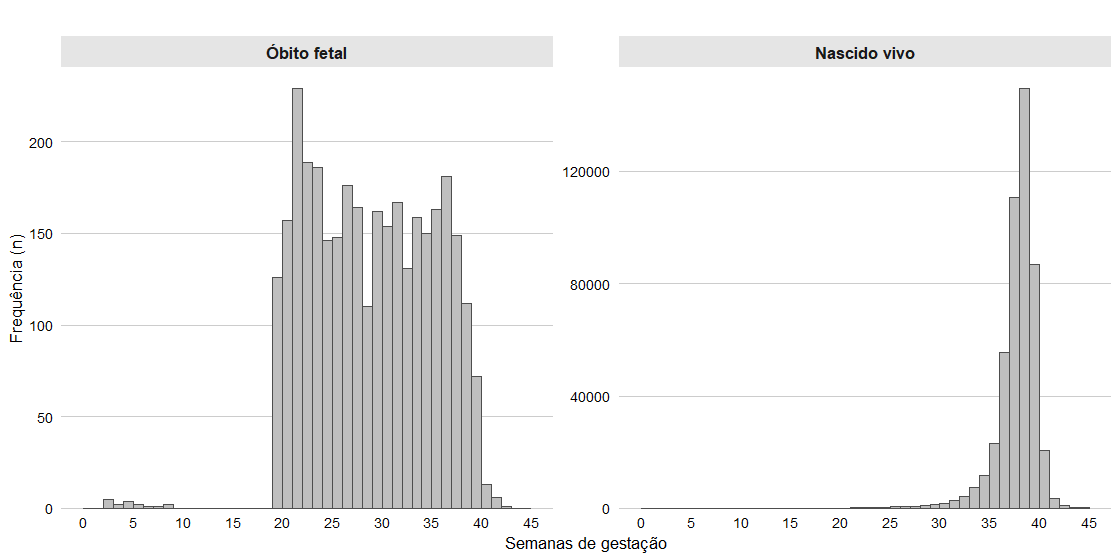
\includegraphics[width=0.9\linewidth]{figuras/histograma_ambas_causas.png}
  \fonte{Fonte: figura feita pelo autor.}
  \label{fig:histograma_ambas_causas}
\end{figure}

Nas curvas globais de Kaplan-Meier (Figura \ref{fig:0_ambos_km_global}), quando 
o óbito fetal é tratado como evento de interesse e o nascimento vivo como censura, 
a função de sobrevivência fica muito próxima de 1 durante toda a gestação, o que 
reforça a raridade desse desfecho. Quando o nascimento vivo é tratado como evento 
e os óbitos fetais como censura, observa-se uma queda acentuada da função de 
sobrevivência a partir do final do terceiro trimestre, mostrando a forte concentração 
dos desfechos em torno do termo.

%---------------------- KM globais
\begin{figure}[H]
  \centering
  \caption{Curvas de Kaplan-Meier da idade gestacional para cada desfecho}
  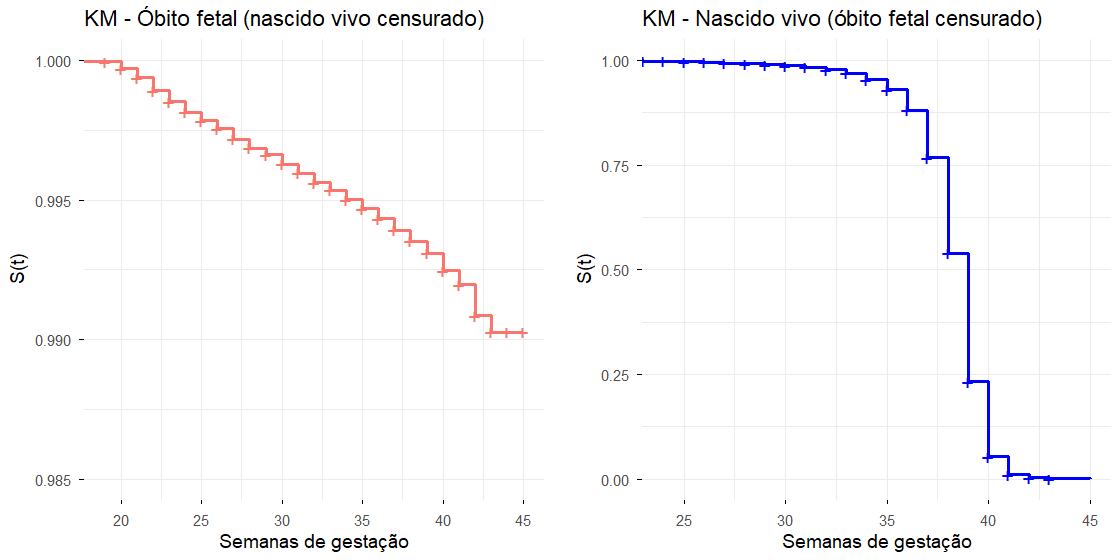
\includegraphics[width=0.9\linewidth]{figuras/0_ambos_km_global.png}
  \fonte{Fonte: figura feita pelo autor.}
  \label{fig:0_ambos_km_global}
\end{figure}

De forma complementar, as funções de incidência acumulada (CIF) por 
causa (Figura \ref{fig:cif_global_painel}) mostram a probabilidade acumulada de 
ocorrência de cada desfecho ao longo da gestação na presença de riscos 
competitivos. Para o óbito fetal, essa incidência permanece baixa em praticamente 
todo o acompanhamento. Em torno de 30 semanas, a probabilidade acumulada de óbito 
fetal foi de aproximadamente 0,37\% (CIF $\approx$ 0,0037) e, mesmo na semana 40, 
manteve-se em torno de 0,66\% (CIF $\approx$ 0,0066), o que corresponde a cerca 
de 7 óbitos fetais por 1.000 gestações.

Já a CIF para nascimento vivo cresce de forma gradual a partir do terceiro trimestre, 
atingindo aproximadamente 1,2\% em 30 semanas (CIF $\approx$ 0,0123) e cerca 
de 94\% na semana 40 (CIF $\approx$ 0,94). Entre 40 e 45 semanas, essa CIF continua 
a crescer até se aproximar de 99\%, indicando que, ao final do acompanhamento, quase 
todas as gestações terminaram em nascimento vivo, enquanto uma pequena fração evoluiu 
para óbito fetal.

%---------------------- CIF globais
\begin{figure}[H]
  \centering
  \caption{Gráficos de incidência acumulada da idade gestacional para cada desfecho.}
  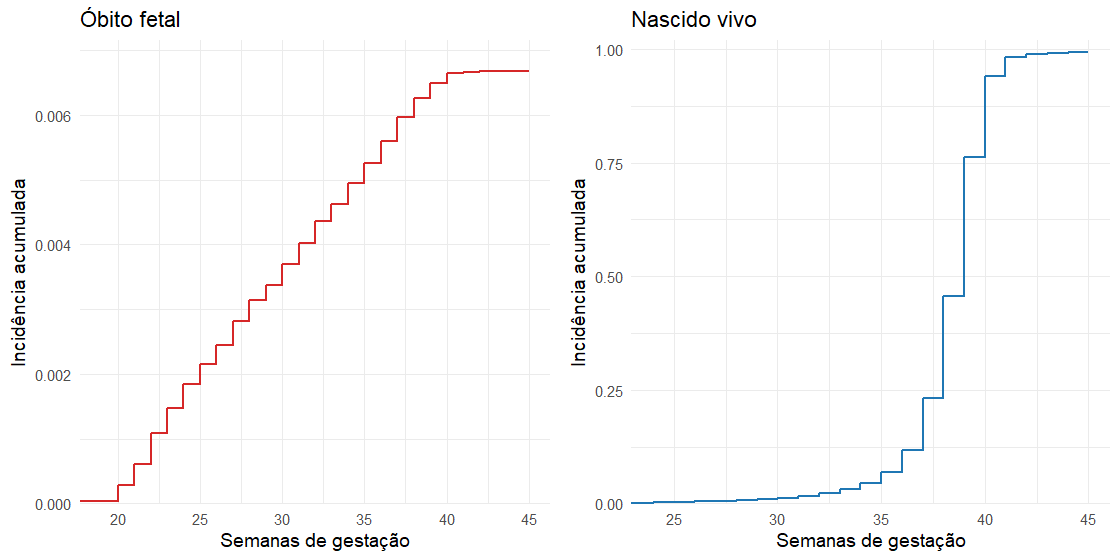
\includegraphics[width=0.9\linewidth]{figuras/cif_global_painel.png}
  \fonte{Fonte: figura feita pelo autor.}
  \label{fig:cif_global_painel}
\end{figure}

\section{Variáveis comuns para as duas causas}

Os resultados descritivos da Tabela \ref{tab:tabela-descritiva-conjunta} já apontam
diferenças entre os grupos de óbito fetal e nascido vivo e indicam heterogeneidade
inicial para a análise de sobrevivência com riscos competitivos. Como o tamanho
amostral é grande, os testes de Log-rank e de Gray tendem a detectar até diferenças
pequenas. Por isso, estatísticas $\chi^2$ muito elevadas e valores-p muito pequenos
devem ser lidos em conjunto com os gráficos e com a magnitude das diferenças
observadas.

\newpage
\begin{table}[H]
\centering
\renewcommand{\arraystretch}{1.1}
\caption{Medidas descritivas e testes de Log-rank (LR) e de Gray (GR).}
\begin{tabular}{lll}
\specialrule{0.16em}{0pt}{0pt}
\textbf{Variáveis numéricas} &
  \begin{tabular}{@{}l@{}}%
  \textbf{Óbito fetal}\\
  Média $\pm$ DP
  \end{tabular} &
  \begin{tabular}{@{}l@{}}
  \textbf{Nascido vivo}\\
  Média $\pm$ DP
  \end{tabular} \\
\specialrule{0.16em}{0pt}{0pt}
Idade materna (idademae)               & 28,92 $\pm$ 7,15 & 28,64 $\pm$ 6,59 \\
Peso ao nascer (peso)                 & 1\,381,68 $\pm$ 996,53 & 3\,132,56 $\pm$ 553,44 \\
Nº de filhos mortos previamente (qtdfilmort)    & 0,56 $\pm$ 0,83 & 0,28 $\pm$ 0,62 \\
Nº de filhos vivos previamente (qtdfilvivo)     & 1,03 $\pm$ 1,37 & 0,93 $\pm$ 1,13 \\
Idade gestacional ao parto (semagestac) & 29,39 $\pm$ 6,19 & 38,26 $\pm$ 2,13 \\
\specialrule{0.16em}{0pt}{0pt}

\textbf{Variáveis categóricas} &
  \begin{tabular}{@{}l@{}}%
    \textbf{Óbito fetal}\\[-3pt]
    {\scriptsize L: $\chi^2$ $(\text{valor-}p)$}\\[-4pt]
    {\scriptsize G: $\chi^2$ $(\text{valor-}p)$}\\[-3pt]
    n (\%)
  \end{tabular} &
  \begin{tabular}{@{}l@{}}%
    \textbf{Nascido vivo}\\[-3pt]
    {\scriptsize L: $\chi^2$ $(\text{valor-}p)$}\\[-4pt]
    {\scriptsize G: $\chi^2$ $(\text{valor-}p)$}\\[-3pt]
    n (\%)
  \end{tabular} \\

\specialrule{0.16em}{0pt}{0pt}

\begin{tabular}{@{}l@{}}Idade materna (idademae)\\< 20 anos\\20--34 anos\\$\geq 35$ anos\end{tabular} &
\begin{tabular}{@{}l@{}}
{\scriptsize L: 47{,}01 (***)};
{\scriptsize G: 40{,}36 (***)}\\
315 (9,6\,\%)\\2\,134 (65,3\,\%)\\817 (25,0\,\%)\end{tabular} &
\begin{tabular}{@{}l@{}}
{\scriptsize L: 5{\,}756 (***)};
{\scriptsize G: 4\,500\,143 (***)}\\
39\,814 (8,2\,\%)\\342\,235 (70,4\,\%)\\103\,873 (21,4\,\%)\end{tabular} \\
\hline

\begin{tabular}{@{}l@{}}Escolaridade materna (escmae2010)\\Baixa\\Média\\Alta\end{tabular} &
\begin{tabular}{@{}l@{}}
{\scriptsize L: 342 (***)};
{\scriptsize G: 344 (***)}\\
688 (21,1\,\%)\\1\,905 (58,3\,\%)\\673 (20,6\,\%)\end{tabular} &
\begin{tabular}{@{}l@{}}
{\scriptsize L: 2{\,}159 (***)};
{\scriptsize G: 1{\,}702{\,}884 (***)}\\
55\,882 (11,5\,\%)\\286\,794 (59,0\,\%)\\143\,246 (29,5\,\%)\end{tabular} \\
\hline

\begin{tabular}{@{}l@{}}Filhos vivos previamente (qtdfilvivo)\\Não\\Sim\end{tabular} &
\begin{tabular}{@{}l@{}}
{\scriptsize L: 1{,}56 (0,212)};
{\scriptsize G: 2{,}09 (0,148)}\\
1\,497 (45,8\,\%)\\1\,769 (54,2\,\%)\end{tabular} &
\begin{tabular}{@{}l@{}}
{\scriptsize L: 1{\,}113 (***)};
{\scriptsize G: 443{\,}511 (***)}\\
216\,635 (44,6\,\%)\\269\,287 (55,4\,\%)\end{tabular} \\
\hline

\begin{tabular}{@{}l@{}}Filhos mortos previamente (qtdfilmort)\\Não\\Sim\end{tabular} &
\begin{tabular}{@{}l@{}}
{\scriptsize L: 765 (***)};
{\scriptsize G: 736 (***)}\\
1\,929 (59,1\,\%)\\1\,337 (40,9\,\%)\end{tabular} &
\begin{tabular}{@{}l@{}}
{\scriptsize L: 1{\,}269 (***)};
{\scriptsize G: 3{\,}306{\,}460 (***)}\\
382\,064 (78,6\,\%)\\103\,858 (21,4\,\%)\end{tabular} \\
\hline

\begin{tabular}{@{}l@{}}Tipo de gestação (gravidez)\\Única\\Múltipla\end{tabular} &
\begin{tabular}{@{}l@{}}
{\scriptsize L: 460 (***)};
{\scriptsize G: 301 (***)}\\
3\,019 (92,4\,\%)\\247 (7,6\,\%)\end{tabular} &
\begin{tabular}{@{}l@{}}
{\scriptsize L: 49{\,}927 (***)};
{\scriptsize G: -2{\,}361 (0{,}99)}\\
473\,046 (97,4\,\%)\\12\,876 (2,6\,\%)\end{tabular} \\
\hline

\begin{tabular}{@{}l@{}}Tipo de parto (parto)\\Vaginal\\Cesáreo\end{tabular} &
\begin{tabular}{@{}l@{}}
{\scriptsize L: 1{\,}334 (***)};
{\scriptsize G: 1{\,}376 (***)}\\
2\,310 (70,7\,\%)\\956 (29,3\,\%)\end{tabular} &
\begin{tabular}{@{}l@{}}
{\scriptsize L: 4{\,}115 (***)};
{\scriptsize G: 314{\,}658 (***)}\\
189\,360 (39,0\,\%)\\296\,562 (61,0\,\%)\end{tabular} \\
\hline

\begin{tabular}{@{}l@{}}Faixa de peso ao nascer (peso)\\< 2\,500 g\\2\,500--3\,999 g\\$\geq 4\,000$ g\end{tabular} &
\begin{tabular}{@{}l@{}}
{\scriptsize L: 24{\,}947 (***)};
{\scriptsize G: 18{\,}759 (***)}\\
2\,720 (83,3\,\%)\\511 (15,6\,\%)\\35 (1,1\,\%)\end{tabular} &
\begin{tabular}{@{}l@{}}
{\scriptsize L: 136{\,}887 (***)};
{\scriptsize G: 5{\,}204{\,}921 (***)}\\
48\,219 (9,9\,\%)\\420\,310 (86,5\,\%)\\17\,393 (3,6\,\%)\end{tabular} \\
\hline

\begin{tabular}{@{}l@{}}Local de ocorrência do parto (lococornasc)\\Hospital\\Outros\end{tabular} &
\begin{tabular}{@{}l@{}}
{\scriptsize L: 287 (***)};
{\scriptsize G: 288 (***)}\\
3\,183 (97,5\,\%)\\83 (2,5\,\%)\end{tabular} &
\begin{tabular}{@{}l@{}}
{\scriptsize L: 39{,}5 (***)};
{\scriptsize G: 71{\,}669{\,}914 (***)}\\
483\,632 (99,5\,\%)\\2\,290 (0,5\,\%)\end{tabular} \\
\hline

\begin{tabular}{@{}l@{}}Sexo do recém-nascido (sexo)\\Masculino\\Feminino\end{tabular} &
\begin{tabular}{@{}l@{}}
{\scriptsize L: 6{,}77 (**)}; 
{\scriptsize G: 6{,}14 (0,013)}\\
1\,738 (53,2\,\%)\\1\,528 (46,8\,\%)\end{tabular} &
\begin{tabular}{@{}l@{}}
{\scriptsize L: 110 (***)};
{\scriptsize G: 750{\,}287 (***)}\\
248\,019 (51,0\,\%)\\237\,903 (49,0\,\%)\end{tabular} \\
\hline

\end{tabular}
\fonte{n (\%): frequências em relação ao total de indivíduos de cada grupo,
considerando registros com informação válida de idade gestacional e da variável.
L e G: testes de Log-rank e de Gray, com estatística do teste ($\chi^2$) e
valor-p. Significância: *** $p<0{,}001$; ** $p<0{,}01$. Fonte: elaboração do
autor.}
\label{tab:tabela-descritiva-conjunta} 
\end{table}

Nas variáveis numéricas, o grupo de óbito fetal apresentou, em média, peso ao
nascer bem menor que o grupo de nascidos vivos (1.381,68 $\pm$ 996,53 e
3.132,56 $\pm$ 553,44, respectivamente), além de idade gestacional ao parto muito
menor (29,39 $\pm$ 6,19 e 38,26 $\pm$ 2,13, respectivamente). Assim, é possível notar que 
os óbitos fetais se concentraram em gestações mais precoces e com pesos menores
no momento do desfecho. Além disso, o número médio de filhos mortos previamente
foi maior nesse grupo (0,56 $\pm$ 0,83 contra 0,28 $\pm$ 0,62 em nascidos vivos),
o que sugere histórico reprodutivo menos favorável em parte dessas gestantes.

Entre as variáveis categóricas, a idade materna chama atenção. O grupo com menos de 20 anos correspondeu a
9,6\% dos óbitos fetais e 8,2\% dos nascidos vivos, no grupo de 20--34 anos esses valores foram de 65,3\% para óbitos fetais e 70,4\% para nascidos vivos, enquanto o grupo com 35 anos 
ou mais correspondeu a 25,0\% e 21,4\%, respectivamente. Nos gráficos de Kaplan-Meier da Figura \ref{fig:kmglobal_idade_mae}, as curvas
por idade materna sugerem diferenças no tempo até o desfecho. Para óbito fetal, o
teste de Log-rank foi significativo ($\chi^2=47{,}01$; $p<0{,}001$). Nos óbitos
fetais, as medianas (Q1--Q3) foram de 28 semanas (24--33) nas gestantes com menos
de 20 anos, 29 semanas (24--35) entre 20 e 34 anos e 30 semanas (24--35) no grupo com 35 anos ou
mais. Para nascimento vivo, o Log-rank também foi significativo
($\chi^2=5\,756$; $p<0{,}001$), com medianas de 39 semanas (38--40), 39 semanas (38--39) e 38 semanas (37--39), respectivamente. 

%---------------------------------------------------------
%---------------------- idademae
%---------------------------------------------------------

%---------------------- KM
\begin{figure}[H]
  \centering
  \caption{Gráficos de Kaplan-Meier da variável idademae para cada desfecho.}
  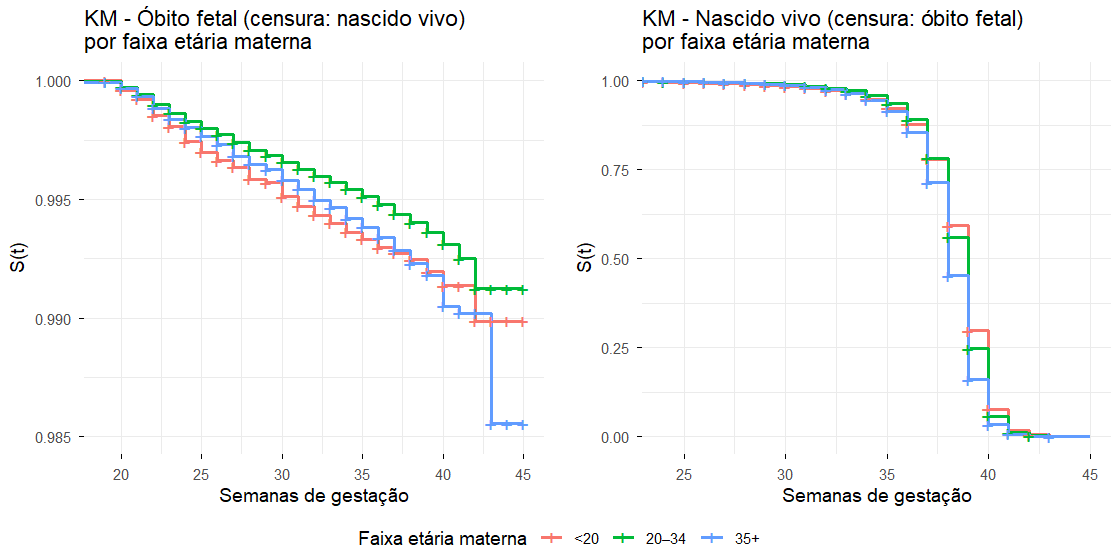
\includegraphics[width=0.9\linewidth]{figuras/kmglobal_idade_mae.png}
  \fonte{Fonte: figura feita pelo autor.}
  \label{fig:kmglobal_idade_mae}
\end{figure}
%---------------------- CIF
Na Figura \ref{fig:cif_idademae_painel_ambos}, sob a perspectiva de óbito fetal, o grupo
com menos de 20 anos apresentou a maior CIF durante grande parte do
acompanhamento: 0,49\% na semana 30, 0,66\% na semana 35 e 0,78\% na semana 40.
No grupo com 35 anos ou mais, os valores foram muito próximos ao final do
seguimento, passando de 0,42\% para 0,61\% e 0,78\%, enquanto o grupo de 20 a 34
anos manteve os menores valores, com 0,34\%, 0,48\% e 0,61\%, respectivamente.
O teste de Gray confirmou evidência de diferença para óbito fetal
($\chi^2=40{,}36$; $p<0{,}001$). Para nascimento vivo, o padrão foi diferente:
na semana 30 a maior CIF apareceu entre as menores de 20 anos (1,66\%), mas a
partir da semana 35 o grupo com 35 anos ou mais passou a concentrar mais
nascimentos vivos, com 8,51\% na semana 35 e 95,92\% na semana 40, contra 7,75\%
e 91,50\% nas menores de 20 anos e 6,46\% e 93,71\% no grupo de 20 a 34 anos. O
teste de Gray também apontou diferença para nascimento vivo
($\chi^2=4\,500\,143$; $p<0{,}001$).
\begin{figure}[H]
  \centering
  \caption{Gráficos de incidência acumulada da variável idademae para cada desfecho.}
  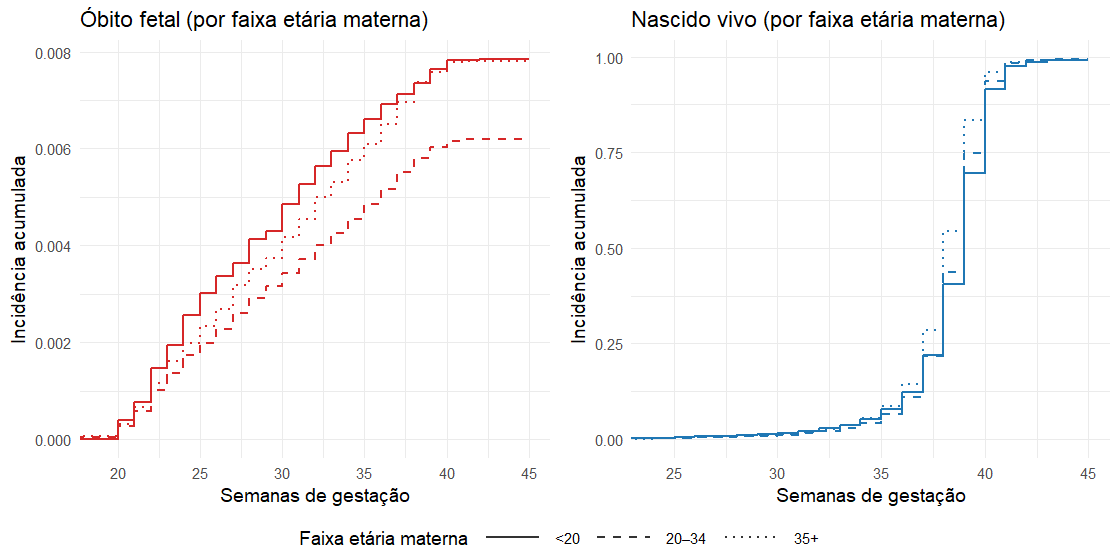
\includegraphics[width=0.9\linewidth]{figuras/cif_idademae_painel_ambos.png}
  \fonte{Fonte: figura feita pelo autor.}
  \label{fig:cif_idademae_painel_ambos}
\end{figure}

Assim, a idade materna apresentou heterogeneidade nos dois desfechos. Na
perspectiva do óbito fetal, o grupo de 20 a 34 anos teve menor probabilidade
acumulada de óbito fetal, enquanto os extremos de idade, especialmente menores de
20 anos durante boa parte do acompanhamento e 35 anos ou mais ao final da
gestação, concentraram resultados menos favoráveis para gestação.

%---------------------------------------------------------
%---------------------- escolaridade
%---------------------------------------------------------

%---------------------- KM
Nos gráficos de Kaplan-Meier da Figura \ref{fig:kmglobal_escmae2010}, a
escolaridade materna sugere diferenças mais visíveis entre as curvas no óbito fetal do que no
nascimento vivo. O Log-rank foi significativo nas duas análises
($\chi^2=342$ para óbito fetal e $\chi^2=2\,159$ para nascimento vivo;
$p<0{,}001$ em ambos), indicando que as curvas não devem ser tratadas como
equivalentes. Nos óbitos fetais, as medianas (Q1--Q3) foram de 30 semanas
(24--35) na baixa escolaridade, 30 semanas (24--35) na escolaridade média e 28 semanas (23--34)
na alta escolaridade. Entre os nascidos vivos, as medianas foram de 39 semanas
em todos os grupos, com intervalo interquartílico de 37--40 na baixa
escolaridade, 38--40 na média e 38--39 na alta.
\begin{figure}[H]
  \centering
  \caption{Gráficos de Kaplan-Meier da variável escmae2010 referente a escolaridade materna,
  para cada desfecho.}
  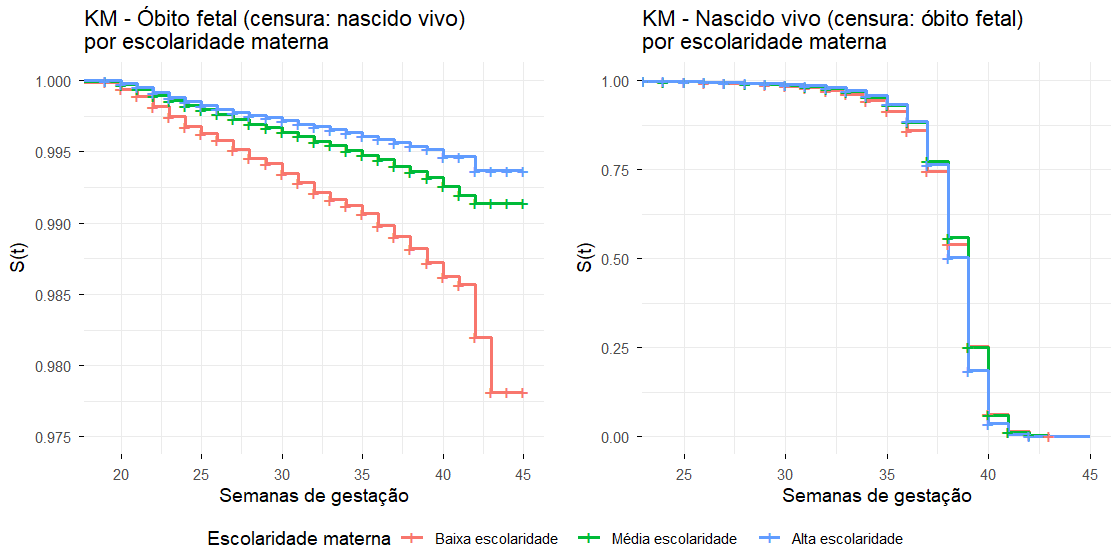
\includegraphics[width=0.9\linewidth]{figuras/kmglobal_escmae2010.png}
  \fonte{Fonte: figura feita pelo autor.}
  \label{fig:kmglobal_escmae2010}
\end{figure}
%---------------------- CIF
Na Figura \ref{fig:cif_escmae2010_painel_ambos}, na semana 40, a CIF de óbito
fetal foi de 1,21\% na baixa escolaridade, 0,66\% na escolaridade média e 0,47\%
na alta escolaridade. O Gray reforçou essa diferença no óbito fetal
($\chi^2=344$; $p<0{,}001$). Entre os nascidos vivos, as curvas também apresentaram diferenças, mas com menor contraste visual, alcançando 92,50\% na baixa
escolaridade, 93,37\% na média e 95,85\% na alta escolaridade na semana 40
($\chi^2=1\,702\,884$; $p<0{,}001$). Em conjunto, os resultados sugerem situação
mais favorável para gestação no grupo de maior escolaridade, embora parte dessa diferença
provavelmente represente condições sociais e assistenciais associadas.
\begin{figure}[H]
  \centering
  \caption{Gráficos de incidência acumulada da variável escmae2010 referente a escolaridade
  materna, para cada desfecho.}
  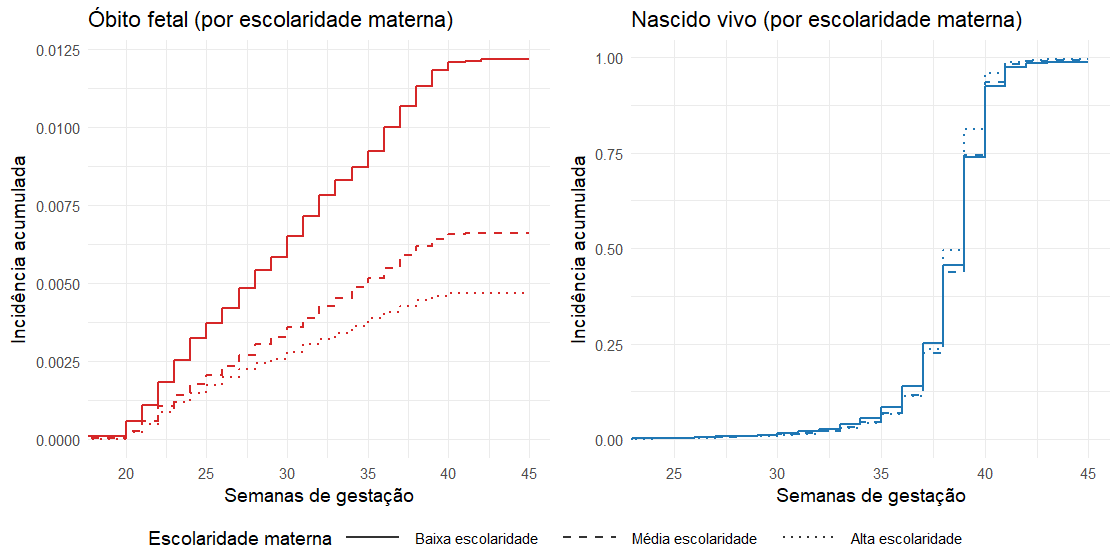
\includegraphics[width=0.9\linewidth]{figuras/cif_escmae2010_painel_ambos.png}
  \fonte{Fonte: figura feita pelo autor.}
  \label{fig:cif_escmae2010_painel_ambos}
\end{figure}

Por tanto, a escolaridade materna aponta para um detalhe importante, com menor
incidência acumulada de óbito fetal e maior concentração de nascimentos vivos no
grupo de maior escolaridade. Esse achado deve ser entendido como marcador de
condições sociais e assistenciais, e não como efeito isolado da escolaridade.

%---------------------------------------------------------
%---------------------- quantidade de filhos vivos
%---------------------------------------------------------

%---------------------- KM
Nos gráficos de Kaplan-Meier da Figura \ref{fig:kmglobal_filvivo}, a presença de
filhos vivos previamente sugere pouco contraste entre os grupos. Essa impressão é coerente com os testes para óbito fetal, que não
foram significativos (Log-rank: $\chi^2=1{,}56$, $p=0{,}212$; Gray:
$\chi^2=2{,}09$, $p=0{,}148$). Para nascimento vivo, o Log-rank foi significativo
($\chi^2=1\,113$; $p<0{,}001$), mas a diferença foi pequena na escala das
semanas. Entre os óbitos fetais, mulheres sem filhos vivos prévios tiveram
mediana de 28 semanas (23--34), enquanto aquelas com esse antecedente tiveram
mediana de 30 semanas (25--35). Entre os nascidos vivos, as medianas foram de 39
semanas nos dois grupos, com Q1--Q3 de 38--40 no grupo sem filhos vivos prévios
e 38--39 no grupo com esse antecedente.
\begin{figure}[H]
  \centering
  \caption{Gráficos de Kaplan-Meier da variável qtdfilvivo referente a quantidade de filhos
  vivos anteriores, para cada desfecho.}
  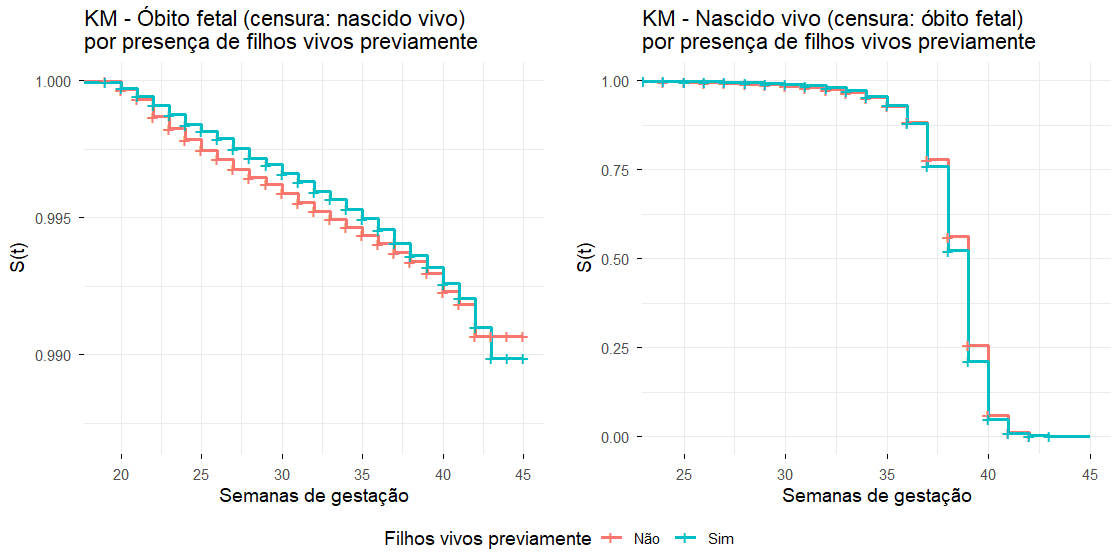
\includegraphics[width=0.9\linewidth]{figuras/kmglobal_filvivo.png}
  \fonte{Fonte: figura feita pelo autor.}
  \label{fig:kmglobal_filvivo}
\end{figure}
%---------------------- CIF
Na Figura \ref{fig:cif_filvivo_painel_ambos}, a incidência acumulada confirma
que o contraste foi pequeno no óbito fetal: na semana 40, a CIF foi de 0,68\%
entre mulheres sem filhos vivos prévios e de 0,65\% entre aquelas com esse
antecedente. Para nascimento vivo, o Gray foi significativo
($\chi^2=443\,511$; $p<0{,}001$), mas as curvas também ficaram próximas. Ao fim
do acompanhamento, o grupo com filhos vivos prévios acumulou proporção
ligeiramente maior de nascimentos até a semana 40 (94,53\% contra 93,34\%).
Portanto, trata-se de diferença estatisticamente detectável apenas na ótica dos
nascidos vivos, mas pequena do ponto de vista absoluto.
\begin{figure}[H]
  \centering
  \caption{Gráficos de incidência acumulada da variável qtdfilvivo referente a quantidade de
  filhos vivos anteriores, para cada desfecho.}
  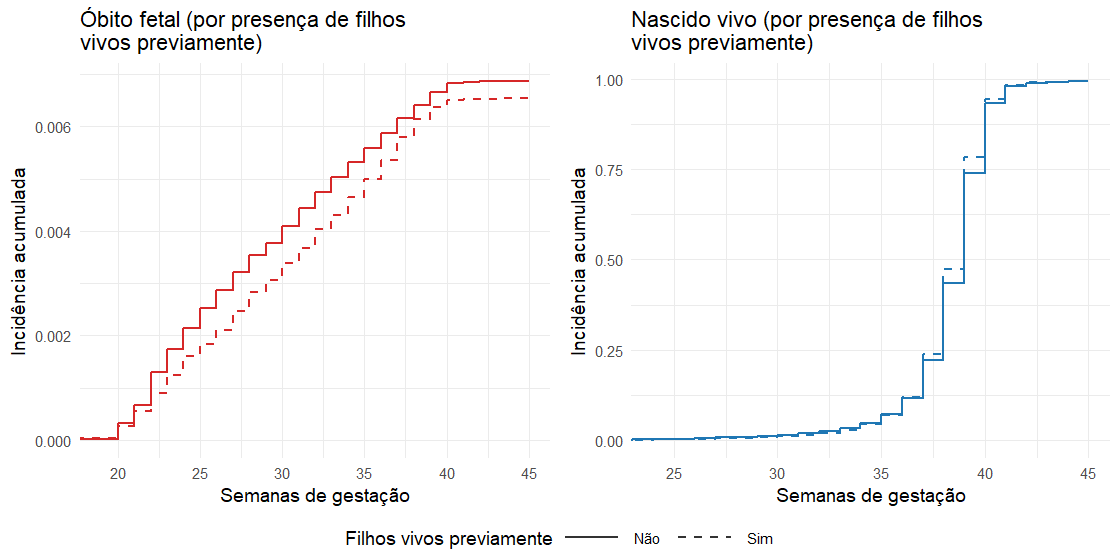
\includegraphics[width=0.9\linewidth]{figuras/cif_filvivo_painel_ambos.png}
  \fonte{Fonte: figura feita pelo autor.}
  \label{fig:cif_filvivo_painel_ambos}
\end{figure}

No geral, a presença de filhos vivos previamente não mostrou um padrão forte
para diferenciar o tempo até o desfecho. A variável parece ter pouca relevância
prática isolada, principalmente para óbito fetal, em que os testes e as curvas
ficaram próximos entre os grupos.

%---------------------------------------------------------
%---------------------- quantidade de filhos mortos
%---------------------------------------------------------

%---------------------- KM
Nos gráficos de Kaplan-Meier da Figura \ref{fig:kmglobal_filmort}, o antecedente
de filhos mortos previamente sugere diferença entre os grupos. O
Log-rank foi significativo para óbito fetal ($\chi^2=765$; $p<0{,}001$) e para
nascimento vivo ($\chi^2=1\,269$; $p<0{,}001$). Descritivamente, entre os óbitos
fetais, gestantes com esse antecedente tiveram mediana de 28 semanas (24--34),
enquanto as demais tiveram mediana de 30 semanas (24--35). Entre os nascidos
vivos, as medianas foram de 38 semanas (37--39) para mulheres com filhos mortos
prévios e de 39 semanas (38--39) para as demais.
\begin{figure}[H]
  \centering
  \caption{Gráficos de Kaplan-Meier da variável qtdfilmort referente a quantidade de filhos
  mortos anteriores, para cada desfecho.}
  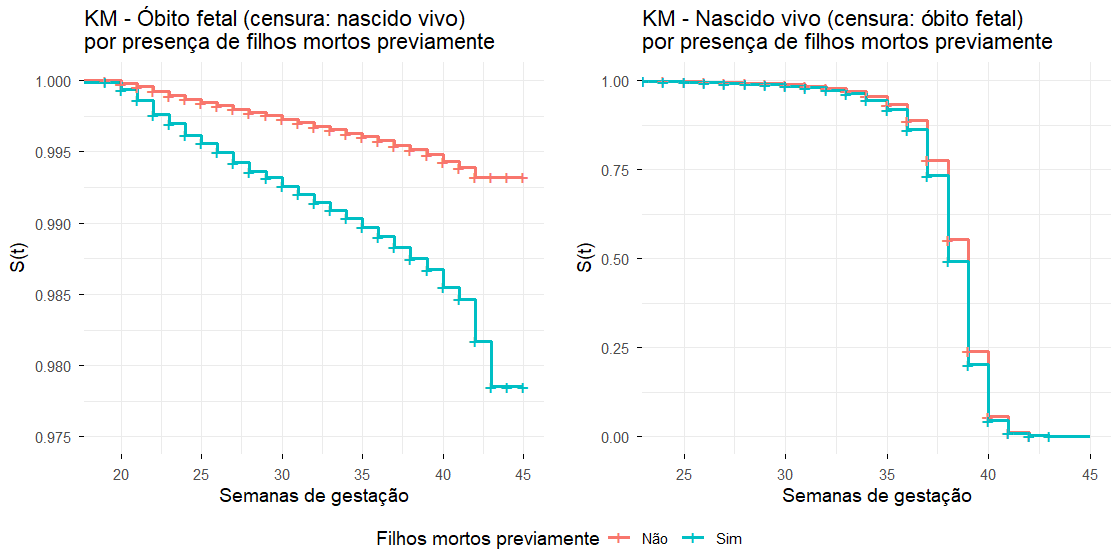
\includegraphics[width=0.9\linewidth]{figuras/kmglobal_filmort.png}
  \fonte{Fonte: figura feita pelo autor.}
  \label{fig:kmglobal_filmort}
\end{figure}
%---------------------- CIF
Na Figura \ref{fig:cif_filmort_painel_ambos}, entre os óbitos fetais, gestantes
com esse antecedente apresentaram CIF mais alta em todas as semanas avaliadas,
passando de 0,74\% na semana 30 para 1,26\% na semana 40, enquanto no grupo sem
esse antecedente os valores foram de 0,27\% e 0,50\%. O teste de Gray para óbito fetal
foi significativo ($\chi^2=736$; $p<0{,}001$). Entre os nascidos vivos, a
diferença foi menor, mas na mesma direção, com CIF de 94,25\% na semana 40 entre
mulheres com filhos mortos prévios e de 93,93\% entre as demais
($\chi^2=3\,306\,460$; $p<0{,}001$). Embora há evidência de diferença entre os grupos, no caso de nascidos vivos os resultados são similares em magnitude.
\begin{figure}[H]
  \centering
  \caption{Gráficos de incidência acumulada da variável qtdfilmort referente a quantidade de
  filhos mortos anteriores, para cada desfecho.}
  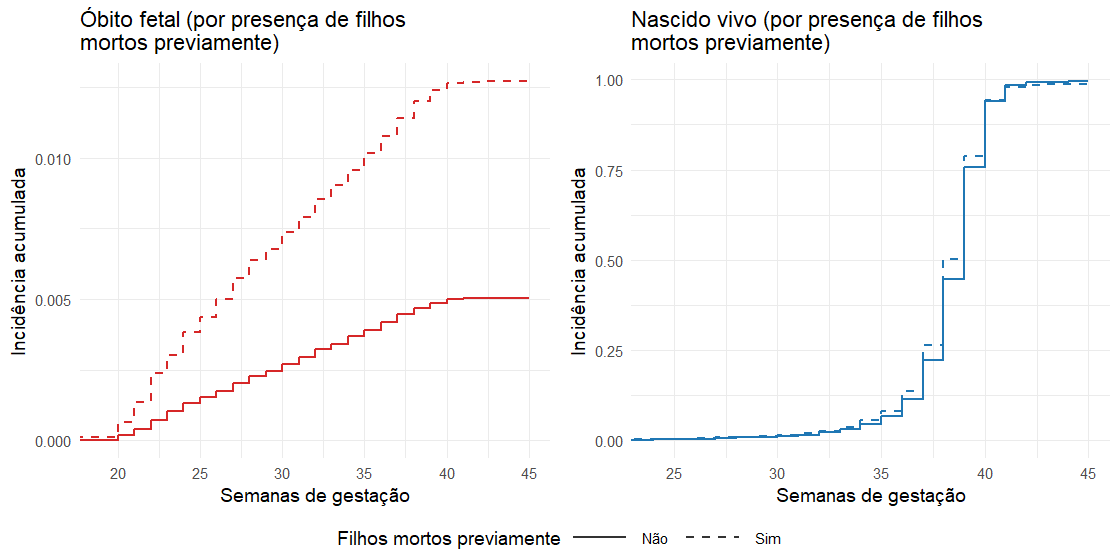
\includegraphics[width=0.9\linewidth]{figuras/cif_filmort_painel_ambos.png}
  \fonte{Fonte: figura feita pelo autor.}
  \label{fig:cif_filmort_painel_ambos}
\end{figure}

Em conjunto, o antecedente de filhos mortos previamente indica um perfil
reprodutivo menos favorável para gestação, sobretudo na ótica de óbito fetal. A maior CIF de óbito
fetal nesse grupo sugere maior vulnerabilidade obstétrica, enquanto nos nascidos
vivos a diferença existiu, mas foi menor em magnitude.

%---------------------------------------------------------
%---------------------- tipo de gravidez
%---------------------------------------------------------

%---------------------- KM
Nos gráficos de Kaplan-Meier da Figura \ref{fig:kmglobal_gravidez}, o tipo de
gestação sugere uma das separações mais claras da análise. De forma descritiva, as
gestações múltiplas terminaram mais cedo que as gestações únicas nas duas
perspectivas. Entre os óbitos fetais, as gestações múltiplas tiveram mediana de
26 semanas (22--32), contra 30 semanas (24--35) nas gestações únicas. Entre os
nascidos vivos, as medianas foram de 36 semanas (34--37) nas múltiplas e 39
semanas (38--39) nas únicas. O Log-rank confirmou forte evidência de diferença entre as curvas 
para óbito fetal ($\chi^2=460$; $p<0{,}001$) e para nascimento vivo
($\chi^2=49\,927$; $p<0{,}001$).
\begin{figure}[H]
  \centering
  \caption{Gráficos de Kaplan-Meier da variável gravidez referente ao tipo de gravidez, para
  cada desfecho.}
  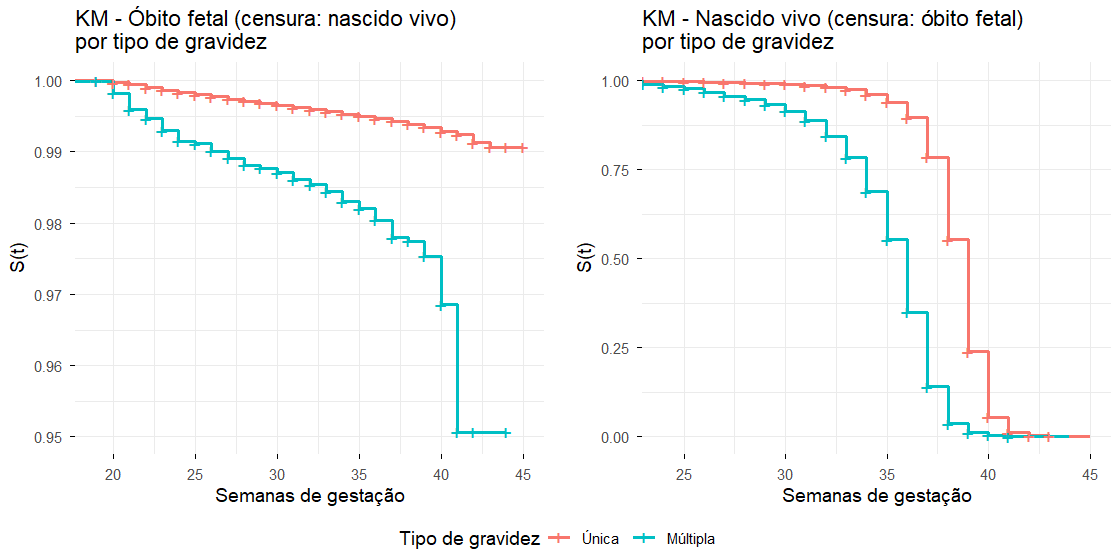
\includegraphics[width=0.9\linewidth]{figuras/kmglobal_gravidez.png}
  \fonte{Fonte: figura feita pelo autor.}
  \label{fig:kmglobal_gravidez}
\end{figure}
%---------------------- CIF
Na Figura \ref{fig:cif_gravidez_painel_ambos}, a CIF permite dimensionar melhor
essa diferença no tempo gestacional. Na ótica do óbito fetal, a incidência
acumulada das gestações múltiplas foi de 1,27\% na semana 30, 1,68\% na semana
35 e 1,87\% na semana 40, enquanto nas gestações únicas os valores foram de
0,34\%, 0,49\% e 0,63\%. O teste de Gray para óbito fetal também apontou diferença 
significativa ($\chi^2=301$; $p<0{,}001$). Para nascimento vivo, a separação foi ainda mais
evidente: nas gestações múltiplas, a CIF já era de 8,51\% na semana 30, chegou a
43,95\% na semana 35 e a 97,71\% na semana 40, contra 1,03\%, 5,99\% e 93,90\%
nas gestações únicas. Assim, esses resultados refletem a maior frequência de
partos pré-termo em gestações múltiplas.
\begin{figure}[H]
  \centering
  \caption{Gráficos de incidência acumulada da variável gravidez referente ao tipo de
  gravidez, para cada desfecho.}
  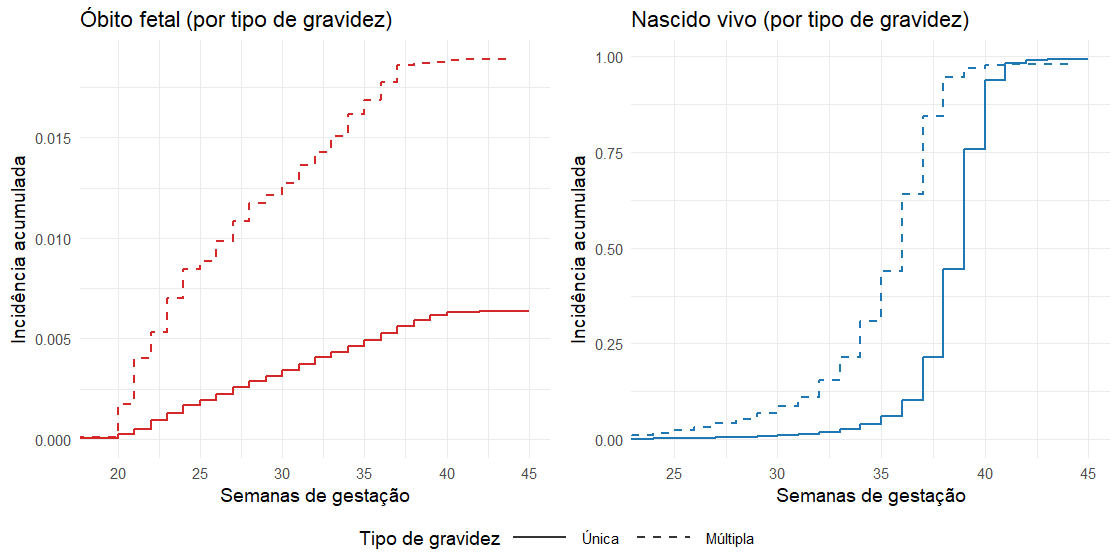
\includegraphics[width=0.9\linewidth]{figuras/cif_gravidez_painel_ambos.png}
  \fonte{Fonte: figura feita pelo autor.}
  \label{fig:cif_gravidez_painel_ambos}
\end{figure}

Portanto, o tipo de gestação foi uma das variáveis com conclusão mais clara:
gestações múltiplas se associaram a desfechos em idades gestacionais mais
precoces e a maior probabilidade acumulada de eventos antes do termo,
principalmente no ambito dos nascidos vivos.

%---------------------------------------------------------
%---------------------- tipo de parto
%---------------------------------------------------------

%---------------------- KM
Nos gráficos de Kaplan-Meier da Figura \ref{fig:kmglobal_parto}, o tipo de parto
sugere distribuições distintas do tempo até o desfecho. O Log-rank foi
significativo para óbito fetal ($\chi^2=1\,334$; $p<0{,}001$) e para nascimento
vivo ($\chi^2=4\,115$; $p<0{,}001$). Nos óbitos fetais, partos vaginais tiveram
mediana de 27 semanas (23--32), enquanto os cesáreos tiveram mediana de 34
semanas (30--37). Entre os nascidos vivos, a mediana foi de 39 semanas nos dois
grupos, mas o intervalo interquartílico foi de 37--39 nos cesáreos e de 38--40
nos vaginais. Como complemento, as médias $\pm$ DP (mediana) foram de 38,15
$\pm$ 2,07 (39) nos cesáreos e 38,41 $\pm$ 2,21 (39) nos vaginais, sugerindo
deslocamento discreto para idades gestacionais um pouco menores no grupo
cesáreo.
\begin{figure}[H]
  \centering
  \caption{Gráficos de Kaplan-Meier da variável parto referente ao tipo de parto, para cada
  desfecho.}
  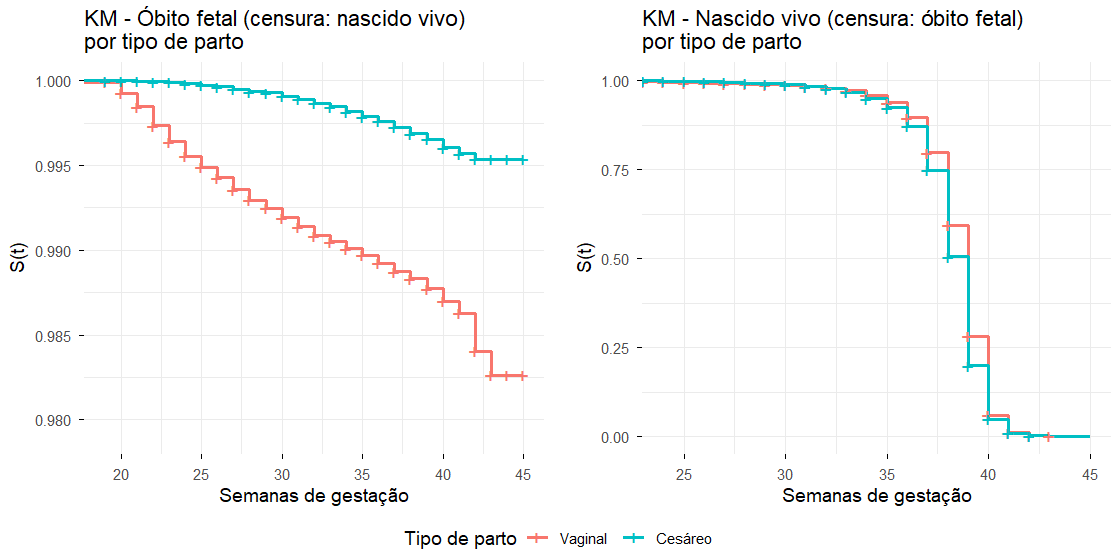
\includegraphics[width=0.9\linewidth]{figuras/kmglobal_parto.png}
  \fonte{Fonte: figura feita pelo autor.}
  \label{fig:kmglobal_parto}
\end{figure}
%---------------------- CIF
Na Figura \ref{fig:cif_parto_painel_ambos}, entre os óbitos fetais, os casos
classificados como parto vaginal se concentraram em idades
gestacionais mais precoces, com CIF de 0,80\% na semana 30 e 1,20\% na semana 40,
contra 0,09\% e 0,32\% entre os partos cesáreos. O teste de Gray para óbito fetal foi
significativo ($\chi^2=1\,376$; $p<0{,}001$). Entre os nascidos vivos, os partos
cesáreos apresentaram incidência acumulada um pouco maior em idades
gestacionais anteriores ou próximas do termo, com CIF de 7,57\% na semana 35 e
94,73\% na semana 40, contra 6,13\% e 92,87\% nos partos vaginais
($\chi^2=314\,658$; $p<0{,}001$). Como o tipo de parto é definido no momento do
desfecho, essa variável deve ser interpretada como parte do processo assistencial
do parto, e não como causa isolada do tempo até o parto.
\begin{figure}[H]
  \centering
  \caption{Gráficos de incidência acumulada da variável parto referente ao tipo de parto,
  para cada desfecho.}
  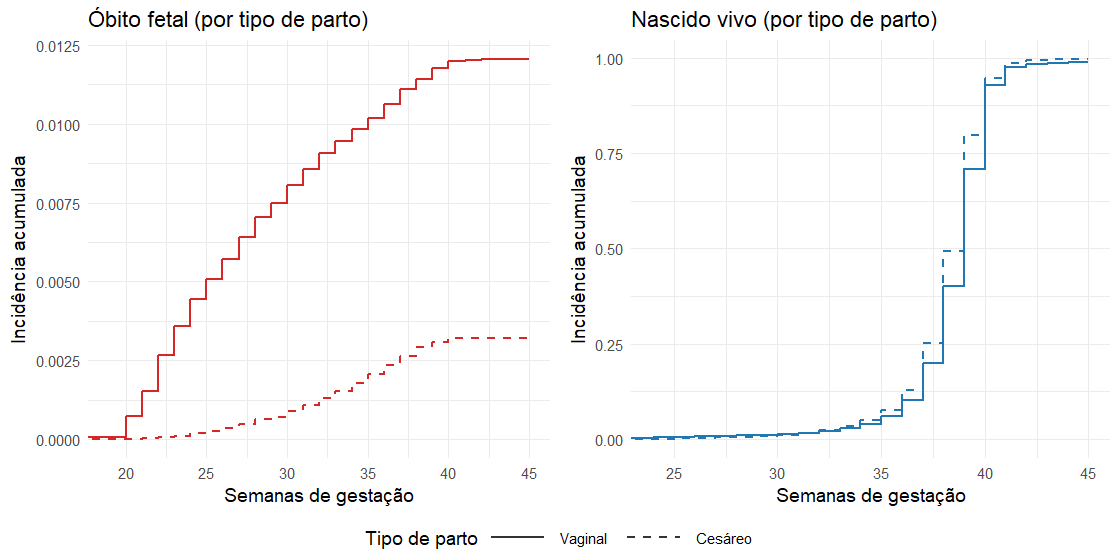
\includegraphics[width=0.9\linewidth]{figuras/cif_parto_painel_ambos.png}
  \fonte{Fonte: figura feita pelo autor.}
  \label{fig:cif_parto_painel_ambos}
\end{figure}

De forma geral, o tipo de parto apresenta diferenças no tempo gestacional, mas sua
interpretação deve permanecer vinculada ao contexto assistencial do parto. Os resultados
mostram associação com o momento do desfecho, principalmente pela concentração de
óbitos fetais mais precoces em partos vaginais e de nascimentos vivos
ligeiramente mais precoces em cesáreas.

%---------------------------------------------------------
%---------------------- peso
%---------------------------------------------------------

%---------------------- KM 
Nos gráficos de Kaplan-Meier da Figura \ref{fig:kmglobal_peso_categorico}, a
faixa de peso ao nascer apresenta o contraste mais evidente entre as variáveis em comuns das bases de dados. O Log-rank foi significativo para óbito fetal ($\chi^2=24\,947$;
$p<0{,}001$) e para nascimento vivo ($\chi^2=136\,887$; $p<0{,}001$). Entre os
óbitos fetais, o grupo com menos de 2.500 g teve mediana de 27 semanas (23--32),
enquanto as faixas de 2.500 a 3.999 g e de 4.000 g ou mais tiveram mediana de 37
semanas, com Q1--Q3 de 36--39 e 36,5--38, respectivamente. Entre os nascidos
vivos, o baixo peso apresentou mediana de 36 semanas (33--37), enquanto as faixas
de 2.500 a 3.999 g e de 4.000 g ou mais tiveram mediana de 39 semanas, com
Q1--Q3 de 38--39 e 39--40.
\begin{figure}[H]
  \centering
  \caption{Gráficos de Kaplan-Meier da variável peso, para cada desfecho.}
  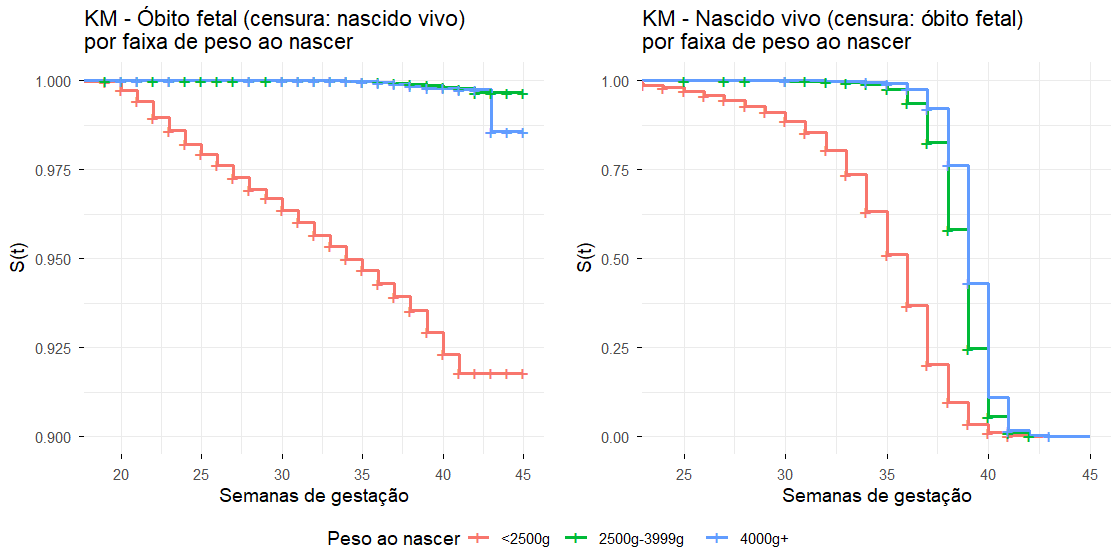
\includegraphics[width=0.9\linewidth]{figuras/kmglobal_peso_categorico.png}
  \fonte{Fonte: figura feita pelo autor.}
  \label{fig:kmglobal_peso_categorico}
\end{figure}
%---------------------- CIF 
Na Figura \ref{fig:cif_peso_categorico_painel_ambos}, entre os óbitos fetais com
peso inferior a 2.500 g, a CIF chegou a 3,52\% na semana 30 e a
5,33\% na semana 40, enquanto nas faixas de 2.500 a 3.999 g e de 4.000 g ou mais
os valores ficaram próximos de zero até o fim do acompanhamento
($\chi^2=18\,759$; $p<0{,}001$ no teste de Gray). Entre os nascidos vivos, o
grupo com menos de 2.500 g também concentrou os desfechos mais precoces,
alcançando CIF de 11,04\% na semana 30 e 46,85\% na semana 35, contra 0,10\% e
2,44\% na faixa de 2.500 a 3.999 g e 0,03\% e 0,85\% na faixa de 4.000 g ou mais
($\chi^2=5\,204\,921$; $p<0{,}001$). Como o peso é observado no momento do
desfecho, essa relação deve ser lida como associação com a idade gestacional, e
não como causa do parto ou do óbito fetal.
\begin{figure}[H]
  \centering
  \caption{Gráficos de incidência acumulada da variável peso, para cada desfecho.}
  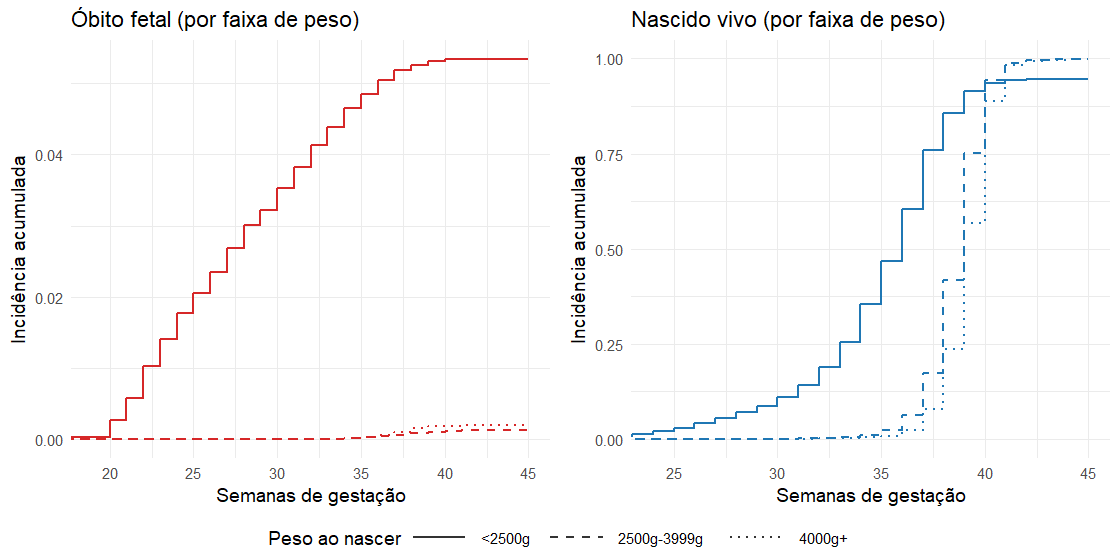
\includegraphics[width=0.9\linewidth]{figuras/cif_peso_categorico_painel_ambos.png}
  \fonte{Fonte: figura feita pelo autor.}
  \label{fig:cif_peso_categorico_painel_ambos}
\end{figure}

Assim, o baixo peso ao nascer foi um dos marcadores mais fortes de
desfechos em idades gestacionais precoces. A interpretação principal é que peso e
idade gestacional estão fortemente relacionados no momento do desfecho, de modo
que essa variável descreve um perfil clínico mais vulnerável, sem indicar
causalidade direta.

%---------------------------------------------------------
%---------------------- local de ocorrência
%---------------------------------------------------------

%---------------------- KM 
Nos gráficos de Kaplan-Meier da Figura \ref{fig:kmglobal_lococornasc}, o local de
ocorrência do parto sugere diferença entre as curvas, mas a interpretação exige
cautela devido ao número muito pequeno de registros fora do hospital. O Log-rank
foi significativo para óbito fetal ($\chi^2=287$; $p<0{,}001$) e para nascimento
vivo ($\chi^2=39{,}5$; $p<0{,}001$). Ainda assim, as medianas observadas foram
iguais entre hospital e outros locais em cada desfecho: 29 semanas para ambos nos óbitos
fetais e 39 semanas nos nascidos vivos. Os intervalos interquartílicos também
foram próximos, de 24--35 e 25--35 nos óbitos fetais, e de 38--39 e 38--40 nos
nascidos vivos, respectivamente.
\begin{figure}[H]
  \centering
  \caption{Gráficos de Kaplan-Meier da variável lococornasc referente ao local de
  ocorrência, para cada desfecho.}
  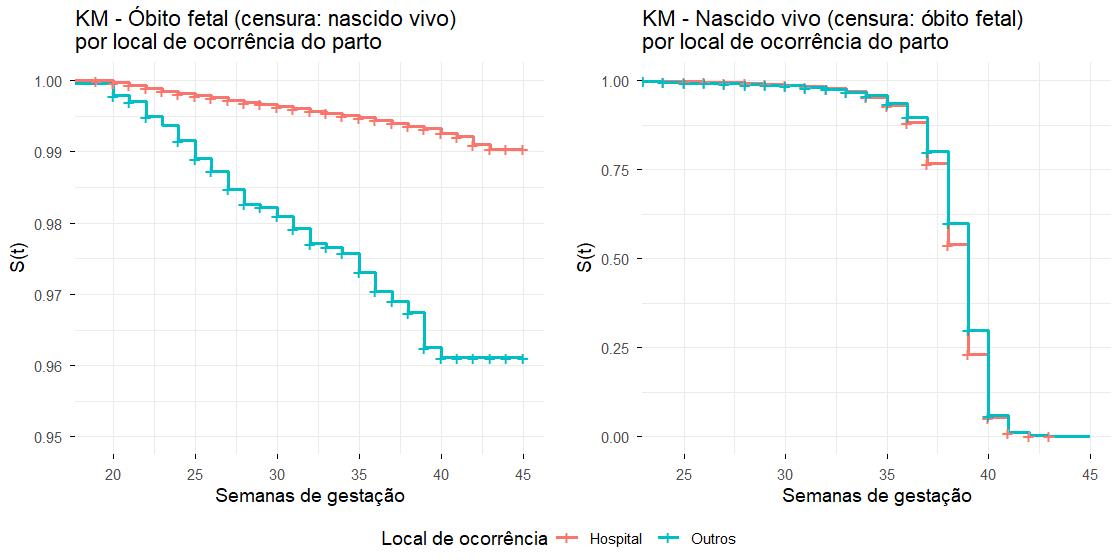
\includegraphics[width=0.9\linewidth]{figuras/kmglobal_lococornasc.png}
  \fonte{Fonte: figura feita pelo autor.}
  \label{fig:kmglobal_lococornasc}
\end{figure}
%---------------------- CIF 
Na Figura \ref{fig:cif_lococornasc_painel_ambos}, a interpretação continua
exigindo cautela porque a categoria ``Outros'' foi muito pequena, com 83 óbitos
fetais e 2.290 nascidos vivos. Mesmo assim, no óbito fetal a CIF foi mais alta
fora do ambiente
hospitalar, chegando a 1,90\% na semana 30 e 3,50\% na semana 40, contra 0,36\%
e 0,65\% nos partos hospitalares ($\chi^2=288$; $p<0{,}001$ no teste de Gray).
Entre os nascidos vivos, a diferença foi menor e menos estável, com CIF de 1,43\%
na semana 30 e 90,94\% na semana 40 nos partos fora do hospital, contra 1,23\% e
94,02\% nos partos hospitalares ($\chi^2=71\,669\,914$; $p<0{,}001$).
\begin{figure}[H]
  \centering
  \caption{Gráficos de incidência acumulada da variável lococornasc referente ao local de
  ocorrência, para cada desfecho.}
  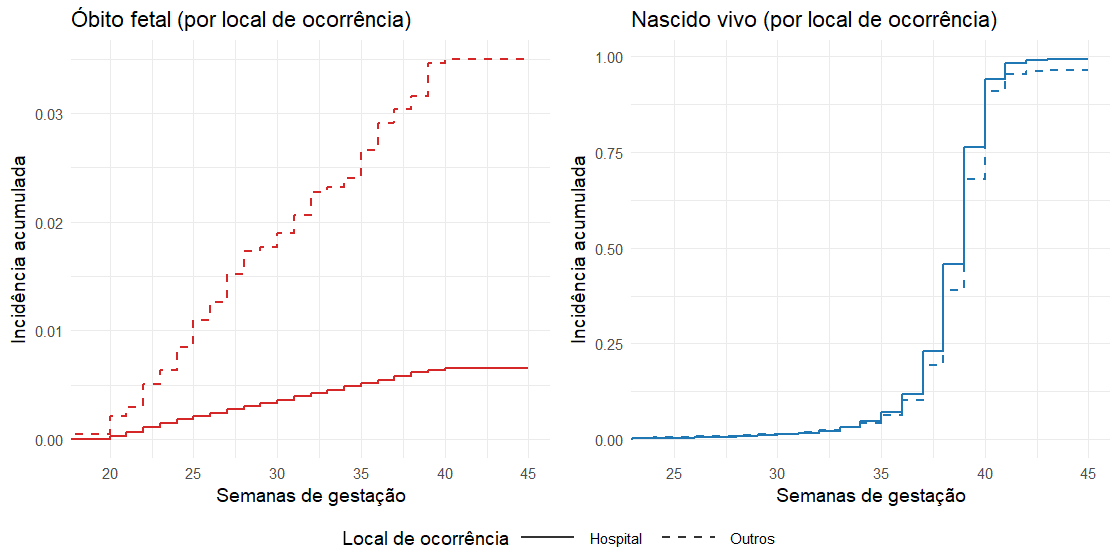
\includegraphics[width=0.9\linewidth]{figuras/cif_lococornasc_painel_ambos.png}
  \fonte{Fonte: figura feita pelo autor.}
  \label{fig:cif_lococornasc_painel_ambos}
\end{figure}

Assim, o local de ocorrência sugere maior acúmulo de óbitos fetais fora do
hospital, mas essa conclusão deve ser vista como exploratória. A baixa frequência
da categoria "Outros" limita a estabilidade da comparação e impede uma leitura
mais forte sobre diferenças.

%---------------------------------------------------------
%---------------------- sexo
%---------------------------------------------------------

%---------------------- KM
Nos gráficos de Kaplan-Meier da Figura \ref{fig:ambos_KM_sexo}, as curvas por
sexo do recém-nascido permanecem bastante próximas. Ainda assim, pelo tamanho da
base, o Log-rank identificou diferença estatística tanto para óbito fetal
($\chi^2=6{,}77$; $p<0{,}01$) quanto para nascimento vivo ($\chi^2=110$;
$p<0{,}001$). Dentro de cada desfecho, porém, as medianas foram iguais entre
meninos e meninas: 29 semanas (24--35) para ambos nos óbitos fetais e 39 semanas (38--39)
nos nascidos vivos. Como complemento, as médias $\pm$ DP (mediana) foram de 29,30
$\pm$ 6,37 (29) no sexo masculino e 29,50 $\pm$ 5,97 (29) no feminino entre os
óbitos fetais, e de 38,22 $\pm$ 2,16 (39) e 38,29 $\pm$ 2,10 (39) entre os
nascidos vivos. Por tanto, é notável que a diferença é pequena em termos
práticos.
\begin{figure}[H]
  \centering
  \caption{Gráficos de Kaplan-Meier da variável sexo para cada desfecho.}
  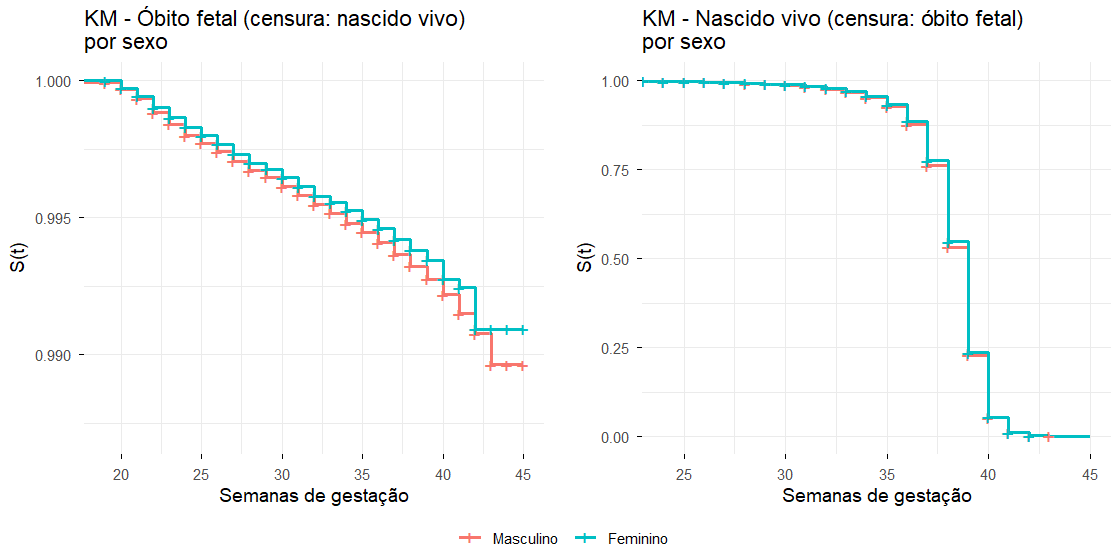
\includegraphics[width=0.9\linewidth]{figuras/kmglobal_sexo.png}
  \fonte{Fonte: figura feita pelo autor.}
  \label{fig:ambos_KM_sexo}
\end{figure}
%---------------------- CIF
Na Figura \ref{fig:ambos_cif_sexo}, as diferenças permaneceram pequenas nas
curvas de incidência acumulada. Entre os óbitos fetais, o sexo masculino teve
frequência um pouco maior (53,2\%) e CIF discretamente superior ao longo do
acompanhamento, chegando a 0,69\% na semana 40, contra 0,63\% no sexo feminino.
O teste de Gray para óbito fetal foi significativo ($\chi^2=6{,}14$; $p=0{,}013$).
Entre os nascidos vivos, as curvas ficaram muito próximas em todo o período, com
CIF de 94,07\% para meninos e 93,93\% para meninas na semana 40, apesar do teste de Gray ser 
significativo ($\chi^2=750\,287$; $p<0{,}001$). Por tanto, a evidência estatística
existe, mas a magnitude absoluta da diferença foi pequena.
\begin{figure}[H]
  \centering
  \caption{Gráficos de incidência acumulada da variável sexo para cada desfecho.}
  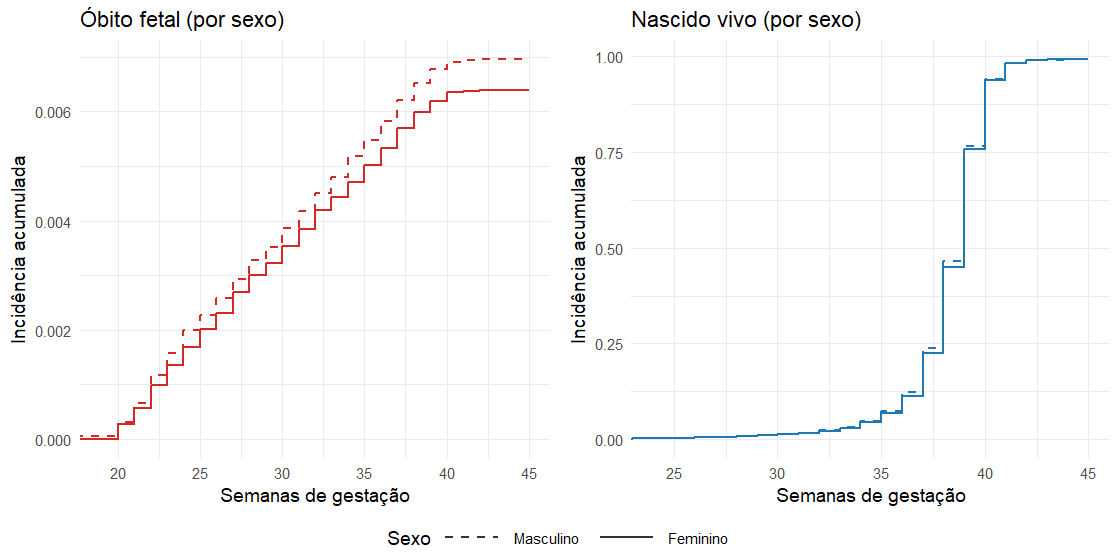
\includegraphics[width=0.9\linewidth]{figuras/ambos_cif_sexo.png}
  \fonte{Fonte: figura feita pelo autor.}
  \label{fig:ambos_cif_sexo}
\end{figure}

Assim, o sexo do recém-nascido apresentou diferenças estatísticas, mas com
pequena importância prática nesta análise. As curvas, medianas e CIF ficaram
muito próximas, indicando que essa variável não foi uma das principais fontes de
diferença no tempo até os desfechos.

Em geral, os resultados das variáveis em comum nas bases de dados mostram que tipo de gestação,
faixa de peso ao nascer e tipo de parto foram os fatores que mais diferenciaram o
tempo até o desfecho. Escolaridade materna, idade materna e antecedente de filhos
mortos também apresentaram contraste relevante, embora menor. Já sexo e presença
de filhos vivos previamente tiveram diferenças pequenas em termos absolutos, e o
local de ocorrência do parto deve ser interpretado com cautela devido ao pequeno
número de registros fora do hospital.

\section{Variáveis exclusivas de cada causa}

A Tabela \ref{tab:tabela-descritiva-exclusivas} reúne as medidas descritivas das
variáveis disponíveis exclusivamente em uma das bases de dados e serve como ponto de partida para 
a leitura dos gráficos de Kaplan-Meier apresentados a seguir.

%---------------- Tabela das variáveis exclusivas
\newpage
\begin{table}[H]
\centering
\renewcommand{\arraystretch}{1.0}
\caption{Medidas descritivas das variáveis exclusivas de cada causa.}
\begin{tabular}{@{}p{0.32\textwidth} p{0.42\textwidth} p{0.16\textwidth}@{}}
\specialrule{0.16em}{0pt}{0pt}
\textbf{Variáveis numéricas} & \textbf{Média $\pm$ DP} & \textbf{Base de dados} \\
\specialrule{0.16em}{0pt}{0pt}
Apgar no 5º minuto (apgar5)                 & 9,41 $\pm$ 0,85   & SINASC \\
Mês de início do pré-natal (mesprenat)     & 2,22 $\pm$ 1,23   & SINASC \\
Nº total de gestações prévias (qtdgestant) & 1,20 $\pm$ 1,36   & SINASC \\
Nº de partos vaginais prévios (qtdpartnor) & 0,55 $\pm$ 1,04   & SINASC \\
Nº de partos cesáreos prévios (qtdpartces) & 0,41 $\pm$ 0,74   & SINASC \\
\specialrule{0.16em}{6pt}{0pt}

\textbf{Variáveis categóricas} & \textbf{Categoria: n (\%)} & \textbf{Base de dados} \\
\specialrule{0.16em}{0pt}{0pt}

Momento do óbito em relação ao parto (obitoparto) &
\begin{tabular}{@{}l@{}}
Antes: 3\,107 (95,1\,\%)\\[-2pt]
Durante: 159 (4,9\,\%)
\end{tabular} &
SIM--DOFET \\
\hline

Apgar no 5º minuto (apgar5) &
\begin{tabular}{@{}l@{}}
$> 7$: 476\,794 (98,1\,\%)\\[-2pt]
$\leq 7$: 9\,128 (1,9\,\%)
\end{tabular} &
SINASC \\
\hline

Consultas de pré-natal (consultas) &
\begin{tabular}{@{}l@{}}
Nenhuma: 468 (0,1\,\%)\\[-2pt]
De 1 a 3: 15\,526 (3,2\,\%)\\[-2pt]
De 4 a 6: 63\,648 (13,1\,\%)\\[-2pt]
7 e mais: 406\,280 (83,6\,\%)
\end{tabular} &
SINASC \\
\hline

Anomalia identificada (idanomal) &
\begin{tabular}{@{}l@{}}
Sim: 7\,550 (1,6\,\%)\\[-2pt]
Não: 478\,372 (98,4\,\%)
\end{tabular} &
SINASC \\
\hline

Início do pré-natal (mesprenat) &
\begin{tabular}{@{}l@{}}
Primeiro trimestre: 432\,864 (89,1\,\%)\\[-2pt]
Segundo trimestre: 46\,020 (9,5\,\%)\\[-2pt]
Terceiro trimestre: 7\,038 (1,4\,\%)
\end{tabular} &
SINASC \\
\hline

Paridade (paridade) &
\begin{tabular}{@{}l@{}}
Nulípara: 184\,346 (37,9\,\%)\\[-2pt]
Multípara: 301\,576 (62,1\,\%)
\end{tabular} &
SINASC \\
\hline

Gestações prévias (qtdgestant) &
\begin{tabular}{@{}l@{}}
Não: 184\,858 (38,0\,\%)\\[-2pt]
Sim: 301\,064 (62,0\,\%)
\end{tabular} &
SINASC \\
\hline

Partos cesáreos prévios (qtdpartces) &
\begin{tabular}{@{}l@{}}
Não: 338\,498 (69,7\,\%)\\[-2pt]
Sim: 147\,424 (30,3\,\%)
\end{tabular} &
SINASC \\
\hline

Partos vaginais prévios (qtdpartnor) &
\begin{tabular}{@{}l@{}}
Não: 333\,278 (68,6\,\%)\\[-2pt]
Sim: 152\,644 (31,4\,\%)
\end{tabular} &
SINASC \\
\hline

Raça/cor da mãe (racacormae) &
\begin{tabular}{@{}l@{}}
Branca: 255\,439 (52,6\,\%)\\[-2pt]
Preta: 39\,259 (8,1\,\%)\\[-2pt]
Amarela: 2\,566 (0,5\,\%)\\[-2pt]
Parda: 188\,113 (38,7\,\%)\\[-2pt]
Indígena: 545 (0,1\,\%)
\end{tabular} &
SINASC \\
\hline

Cesárea antes do trabalho de parto (stcesparto) &
\begin{tabular}{@{}l@{}}
Sim: 198\,839 (40,9\,\%)\\[-2pt]
Não: 97\,723 (20,1\,\%)\\[-2pt]
Não se aplica: 189\,360 (39,0\,\%)
\end{tabular} &
SINASC \\
\hline

Trabalho de parto induzido (sttrabpart) &
\begin{tabular}{@{}l@{}}
Sim: 95\,508 (19,7\,\%)\\[-2pt]
Não: 390\,414 (80,3\,\%)
\end{tabular} &
SINASC \\
\specialrule{0.16em}{0pt}{0pt}
\end{tabular}
\fonte{Média $\pm$ DP (desvio padrão) das variáveis numéricas. n (\%): frequências em
relação ao total de indivíduos de cada grupo. Fonte: elaboração do autor.}
\label{tab:tabela-descritiva-exclusivas}
\end{table}

%---------------------------------------------------------
%---------------------- momento do óbito (em relação ao parto)
%---------------------------------------------------------

Na Figura \ref{fig:km_obitos_obitoparto}, as curvas de Kaplan-Meier sugerem que
o momento do óbito em relação ao parto distingue o tempo até o desfecho. Os
óbitos classificados como ocorridos durante o parto se concentraram em idades
gestacionais mais precoces, com mediana de 24 semanas (22--33), enquanto os
óbitos anteriores ao parto apresentaram mediana de 30 semanas (24--35). O teste
de Log-rank indicou diferença estatística
($\chi^2=7{,}22$; $p=0{,}007$). Ainda assim, a grande maioria dos registros
correspondeu a óbitos anteriores ao parto (95,1\%), como mostra a Tabela
\ref{tab:tabela-descritiva-exclusivas}.
\begin{figure}[H]
  \centering
  \caption{Gráfico de Kaplan-Meier da variável obitoparto referente ao momento do óbito em
  relação ao parto.}
  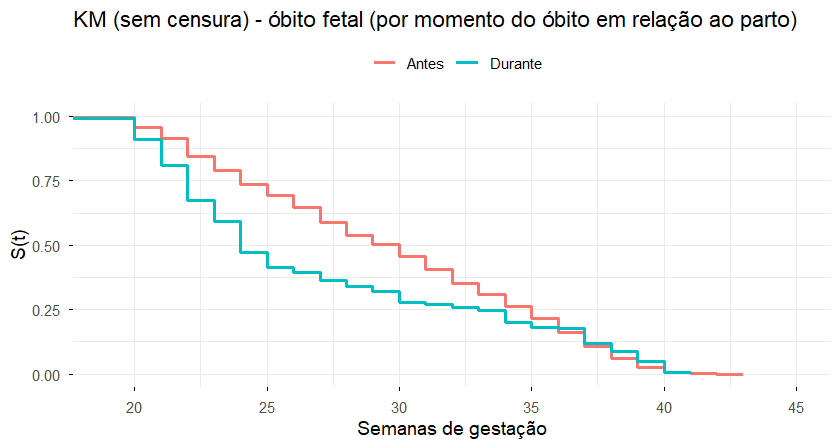
\includegraphics[width=0.9\linewidth]{figuras/km_obitos_obitoparto.png}
  \fonte{Fonte: figura feita pelo autor.}
  \label{fig:km_obitos_obitoparto}
\end{figure}

Assim, embora a maioria dos óbitos fetais tenha ocorrido antes do parto, os poucos 
casos classificados como ocorridos durante o parto aconteceram, em média/mediana, em 
idades gestacionais mais precoces. Portanto, essas categorias parecem representar 
situações obstétricas diferentes dentro dos óbitos fetais, identificando subgrupos 
distintos.

%---------------------------------------------------------
%---------------------- apgar5
%---------------------------------------------------------

Na Figura \ref{fig:km_nascidosvivos_apgar}, as curvas de Kaplan-Meier sugerem, em 
um primeiro momento, diferença entre as curvas. Entre os nascidos vivos, recém nascidos 
com Apgar no quinto minuto igual ou inferior a 7 apresentaram partos em idades
gestacionais menores. Nesse grupo, a mediana foi de 37 semanas (32--39), contra 
39 semanas (38--39) no grupo com Apgar acima de 7. O Log-rank foi 
significativo ($\chi^2=3\,781$; $p<0{,}001$). Embora esse contraste seja nítido, o Apgar 
é medido após o nascimento. Portanto, esse resultado deve ser entendido como marcador de 
pior condição neonatal associado à prematuridade, e não como fator anterior ao tempo 
até o parto.
\begin{figure}[H]
  \centering
  \caption{Gráfico de Kaplan-Meier da variável apgar5 referente ao índice de Apgar no quinto
  minuto.}
  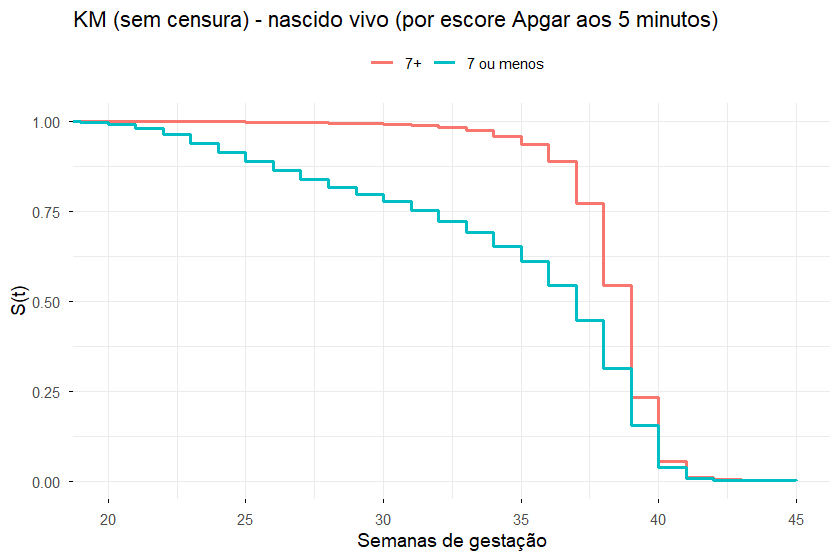
\includegraphics[width=0.9\linewidth]{figuras/km_nascidosvivos_apgar.png}
  \fonte{Fonte: figura feita pelo autor.}
  \label{fig:km_nascidosvivos_apgar}
\end{figure}

No geral, o Apgar no quinto minuto resume um contraste clínico importante entre
os nascidos vivos. Valores menores ou iguais a 7 estiveram ligados a partos mais
precoces e a pior condição neonatal imediata, funcionando mais como marcador do
estado do recém-nascido do que como variável anterior ao parto.

%---------------------------------------------------------
%---------------------- Número de consultas pré-natal
%---------------------------------------------------------

Na Figura \ref{fig:km_nascidosvivos_consultas}, as curvas de Kaplan-Meier
sugerem diferenças mais claras segundo o número de consultas pré-natais. No
grupo com 7 ou mais consultas, a mediana foi de 39 semanas (38--39). Nos grupos
com nenhuma, de 1 a 3 e de 4 a 6 consultas, as medianas foram de 38 semanas, com
intervalos interquartílicos de 37--39, 36--39 e 37--39, respectivamente. O
Log-rank foi significativo ($\chi^2=6\,412$; $p<0{,}001$).
\begin{figure}[H]
  \centering
  \caption{Gráfico de Kaplan-Meier da variável consultas referente ao número de consultas
  pré-natal.}
  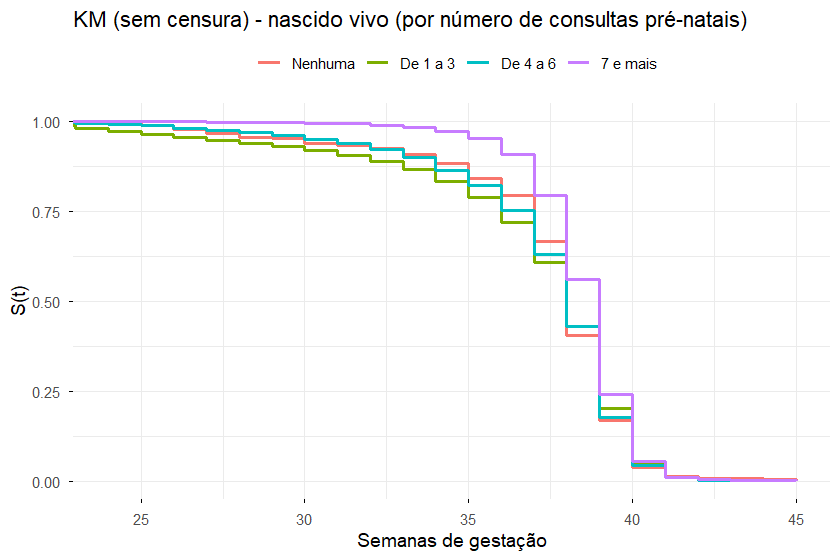
\includegraphics[width=0.9\linewidth]{figuras/km_nascidosvivos_consultas.png}
  \fonte{Fonte: figura feita pelo autor.}
  \label{fig:km_nascidosvivos_consultas}
\end{figure}

Por tanto, o número de consultas pré-natais diferenciou ligeiramente o tempo até o
nascimento vivo, com partos mais precoces entre gestações com menor número de
consultas. Partos prematuros deixam menos tempo para a gestante realizar várias 
consultas. Então, a associação entre poucas consultas e parto mais precoce pode 
refletir tanto falhas de acompanhamento quanto a própria menor duração da 
gestação. Por isso, não devemos concluir automaticamente que mais consultas, sozinhas, 
causam partos mais tardios. Além disso, embora tenha sido detectado diferença entre as 
curvas através do Log-Rank, a diferença em magnitude é sutil.


%---------------------------------------------------------
%---------------------- Anomalia identificada
%---------------------------------------------------------

Na Figura \ref{fig:km_nascidosvivos_anomalia}, as curvas de Kaplan-Meier não sugerem
uma diferença muito clara entre as curvas. Porém, a presença de anomalia identificada 
parece se associar a partos mais precoces. O grupo com anomalia apresentou mediana de 
38 semanas (37--39), contra 39 semanas (38--39) na ausência de anomalia. O Log-rank foi 
significativo ($\chi^2=605$; $p<0{,}001$).
\begin{figure}[H]
  \centering
  \caption{Gráfico de Kaplan-Meier da variável idanomal referente a anomalia identificada.}
  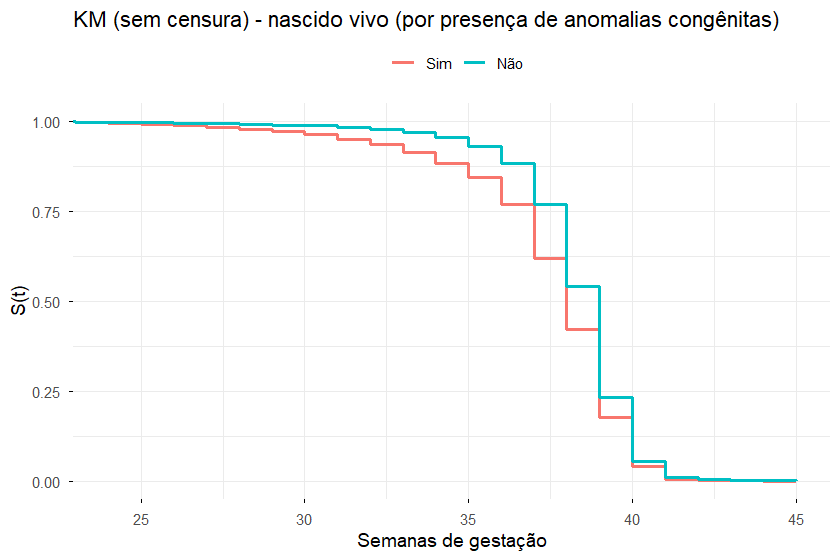
\includegraphics[width=0.9\linewidth]{figuras/km_nascidosvivos_anomalia.png}
  \fonte{Fonte: figura feita pelo autor.}
  \label{fig:km_nascidosvivos_anomalia}
\end{figure}

Por tanto, há algum indício de que a presença de anomalia identificada esteve 
associada a nascimentos em idades gestacionais menores. Esse resultado sugere 
um grupo de maior complexidade clínica, possivelmente relacionado tanto à condição 
fetal quanto a decisões assistenciais de interrupção mais precoce.

%---------------------------------------------------------
%---------------------- Mês de gestação em que se iniciou o pré-natal
%---------------------------------------------------------

Na Figura \ref{fig:km_nascidosvivos_mesprenat}, as curvas de Kaplan-Meier
sugerem diferença segundo o trimestre de início do pré-natal, embora as medianas
tenham permanecido em 39 semanas em todos os grupos. O intervalo interquartílico
foi de 38--39 para início no primeiro trimestre e de 38--40 para início no
segundo e no terceiro. Como complemento, as médias $\pm$ DP (mediana) foram de
38,26 $\pm$ 2,11 (39), 38,19 $\pm$ 2,37 (39) e 38,32 $\pm$ 1,93 (39),
respectivamente. O Log-rank foi significativo ($\chi^2=70{,}90$; $p<0{,}001$),
mas a principal diferença foi pequena e sugere partos ligeiramente mais precoces
entre mulheres que iniciaram o acompanhamento no segundo trimestre. Como o grupo
com início no terceiro trimestre foi bem menor, essa interpretação deve ser
feita com cautela.
\begin{figure}[H]
  \centering
  \caption{Gráfico de Kaplan-Meier da variável mesprenat referente ao mês de gestação em que
  se iniciou o pré-natal.}
  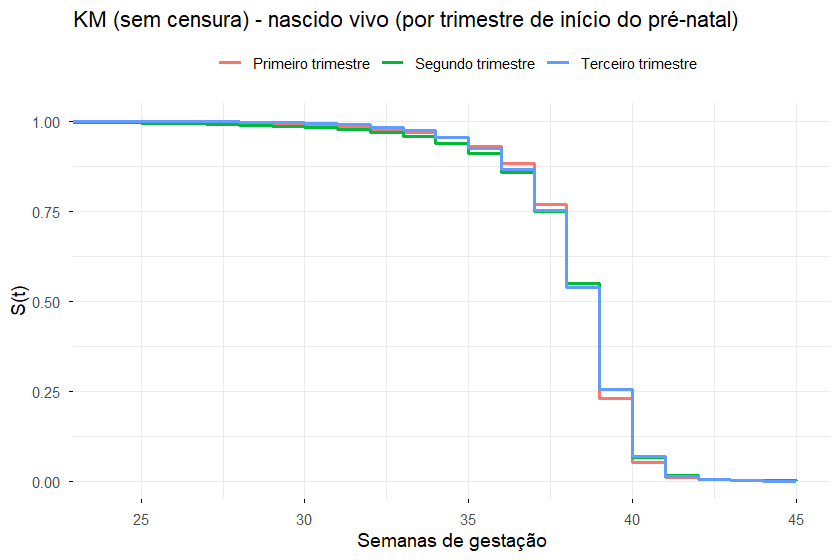
\includegraphics[width=0.9\linewidth]{figuras/km_nascidosvivos_mesprenat.png}
  \fonte{Fonte: figura feita pelo autor.}
  \label{fig:km_nascidosvivos_mesprenat}
\end{figure}

Assim, o trimestre de início do pré-natal mostrou diferença estatística, mas com
pequena magnitude na escala de semanas. Por tanto, essa variável deve ser lida 
como parte do contexto de acesso e acompanhamento da gestação, sem indicar, 
isoladamente, grande mudança no tempo até o nascimento.

%---------------------------------------------------------
%---------------------- Paridade
%---------------------------------------------------------

Na Figura \ref{fig:km_nascidosvivos_paridade}, as curvas de Kaplan-Meier sugerem
diferença discreta segundo a paridade. A mediana foi de 39 semanas nos dois
grupos, com intervalo interquartílico de 38--40 nas nulíparas e 38--39 nas
multíparas. Como complemento, as médias $\pm$ DP (mediana) foram de 38,34
$\pm$ 2,20 (39) e 38,20 $\pm$ 2,08 (39), respectivamente. O Log-rank foi
significativo ($\chi^2=1\,618$; $p<0{,}001$), mas a magnitude absoluta dessa
diferença foi pequena.
\begin{figure}[H]
  \centering
  \caption{Gráfico de Kaplan-Meier da variável paridade referente a se é a primeira gravidez
  ou se teve mais de uma.}
  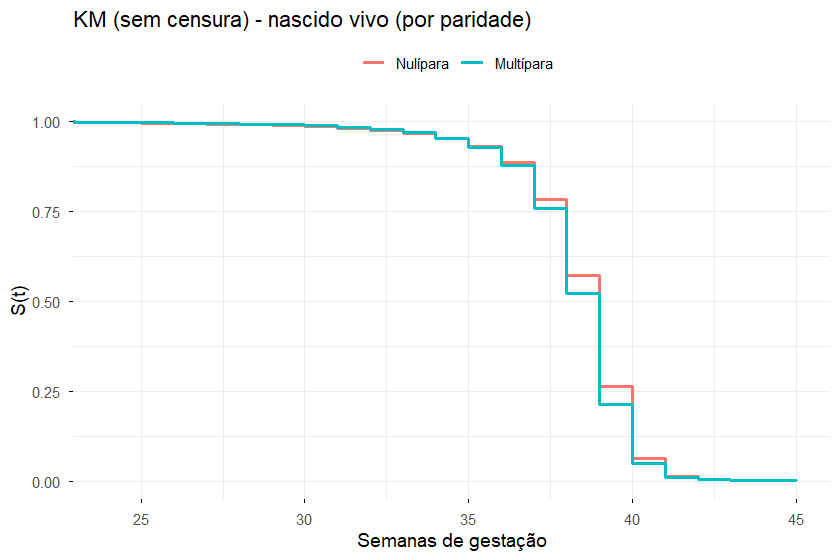
\includegraphics[width=0.9\linewidth]{figuras/km_nascidosvivos_paridade.png}
  \fonte{Fonte: figura feita pelo autor.}
  \label{fig:km_nascidosvivos_paridade}
\end{figure}

No geral, a paridade apresentou diferença detectável, mas discreta. A condição
de nulípara ou multípara, isoladamente, não pareceu modificar de forma importante
o tempo gestacional até o nascimento vivo nesta análise.

%---------------------------------------------------------
%---------------------- Número total de gestações anteriores
%---------------------------------------------------------

Na Figura \ref{fig:km_nascidosvivos_qtdgestant}, as curvas de Kaplan-Meier
sugerem diferença segundo a presença de gestações anteriores, embora com pequena
magnitude. A mediana foi de 39 semanas nos dois grupos, com Q1--Q3 de 38--40 nas
mulheres sem gestações prévias e 38--39 naquelas com história gestacional prévia.
Como complemento, as médias $\pm$ DP (mediana) foram de 38,34 $\pm$ 2,20 (39) e
38,20 $\pm$ 2,08 (39), respectivamente. O Log-rank foi significativo
($\chi^2=1\,614$; $p<0{,}001$), mas a diferença absoluta foi pequena.
\begin{figure}[H]
  \centering
  \caption{Gráfico de Kaplan-Meier da variável qtdgestant referente ao número total de
  gestações anteriores.}
  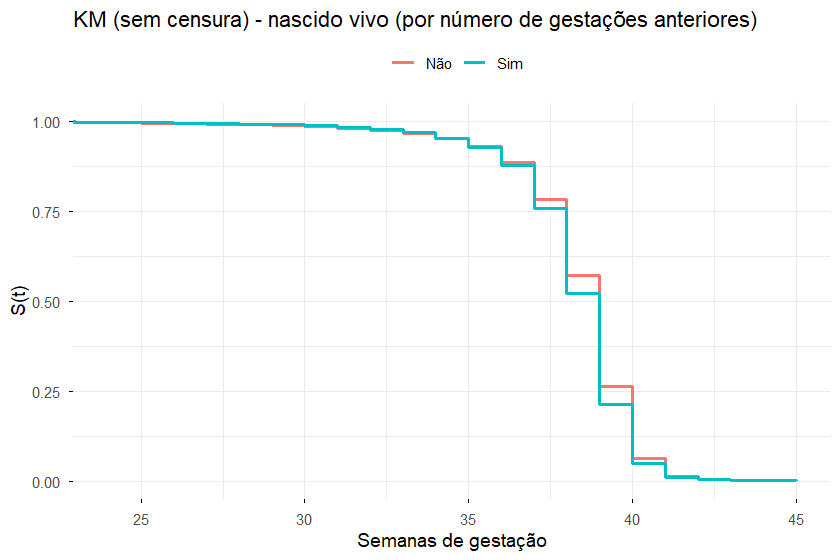
\includegraphics[width=0.9\linewidth]{figuras/km_nascidosvivos_qtdgestant.png}
  \fonte{Fonte: figura feita pelo autor.}
  \label{fig:km_nascidosvivos_qtdgestant}
\end{figure}

De forma semelhante à paridade, a presença de gestações anteriores indicou
diferença estatística pequena. O resultado sugere que o histórico gestacional
prévio, quando avaliado apenas por essa categorização, teve pouca expressão
prática sobre a idade gestacional ao nascimento.

%---------------------------------------------------------
%---------------------- Número total de partos cesáreos anteriores
%---------------------------------------------------------

Na Figura \ref{fig:km_nascidosvivos_qtdpartces}, as curvas de Kaplan-Meier não 
deixam evidente se existe diferença significativa, mas há indícios de que o 
histórico de cesarianas prévias esteve associada a partos discretamente mais 
precoces. Mulheres com cesariana anterior apresentaram mediana de 38 
semanas (38--39), contra 39 semanas (38--40) nas demais. O Log-rank foi 
significativo ($\chi^2=3\,071$; $p<0{,}001$).
\begin{figure}[H]
  \centering
  \caption{Gráfico de Kaplan-Meier da variável qtdpartces referente ao número total de
  partos cesáreos anteriores.}
  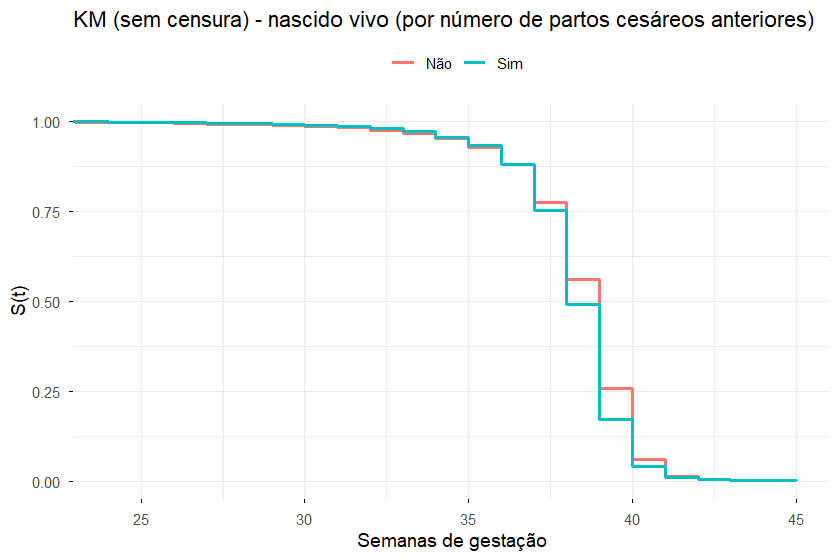
\includegraphics[width=0.9\linewidth]{figuras/km_nascidosvivos_qtdpartces.png}
  \fonte{Fonte: figura feita pelo autor.}
  \label{fig:km_nascidosvivos_qtdpartces}
\end{figure}

Assim, há indícios de que o histórico de cesariana anterior se associa a nascimentos um pouco
mais precoces.

%---------------------------------------------------------
%---------------------- Número total de de partos vaginais anteriores.
%---------------------------------------------------------

Na Figura \ref{fig:km_nascidosvivos_qtdpartnor}, as curvas de Kaplan-Meier
sugerem pouca diferença segundo o número de partos vaginais anteriores. O teste
de Log-rank foi significativo ($\chi^2=46{,}74$; $p<0{,}001$), mas as medianas
foram de 39 semanas em ambos os grupos, com Q1--Q3 de 38--39. As médias $\pm$ DP
(mediana) praticamente coincidiram: 38,26 $\pm$ 2,12 (39) entre mulheres sem
partos vaginais prévios e 38,25 $\pm$ 2,16 (39) entre aquelas com esse
antecedente. Isso sugere pouca relevância clínica nessa diferença.
\begin{figure}[H]
  \centering
  \caption{Gráfico de Kaplan-Meier da variável qtdpartnor referente ao número total de
  partos vaginais anteriores.}
  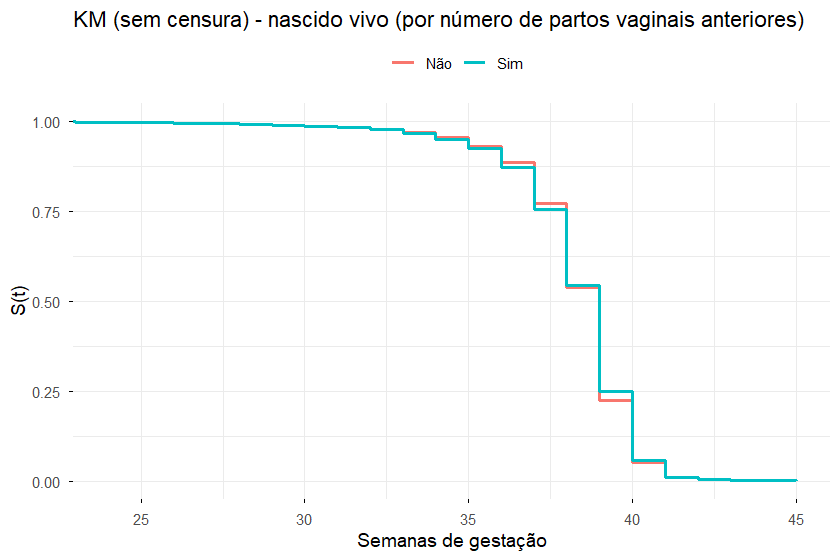
\includegraphics[width=0.9\linewidth]{figuras/km_nascidosvivos_qtdpartnor.png}
  \fonte{Fonte: figura feita pelo autor.}
  \label{fig:km_nascidosvivos_qtdpartnor}
\end{figure}

Por tanto, o número de partos vaginais anteriores apresentou pouca contribuição para
diferenciar a idade gestacional ao nascimento. Apesar da significância
estatística, as medidas descritivas praticamente coincidiram entre os grupos.

%---------------------------------------------------------
%---------------------- Raça/cor da mãe
%---------------------------------------------------------

Na Figura \ref{fig:km_nascidosvivos_racamae}, as curvas de Kaplan-Meier sugerem
diferença estatística global para raça/cor da mãe, mas com curvas bastante
próximas e mediana de 39 semanas em todos os grupos. O Log-rank foi significativo
($\chi^2=943$; $p<0{,}001$). Os intervalos interquartílicos foram muito
próximos: 38--39 em brancas e amarelas e 38--40 em pretas, pardas e indígenas.
Como complemento, as médias $\pm$ DP (mediana) variaram pouco, de 38,22
$\pm$ 2,07 (39) entre brancas a 38,51 $\pm$ 1,83 (39) entre indígenas. Assim,
embora exista heterogeneidade detectável, sua magnitude prática foi pequena
nesta análise descritiva, especialmente diante do grande tamanho amostral e do
baixo número de observações em algumas categorias, como indígenas e amarelas.
\begin{figure}[H]
  \centering
  \caption{Gráfico de Kaplan-Meier da variável racacormae referente a raça/cor da mãe.}
  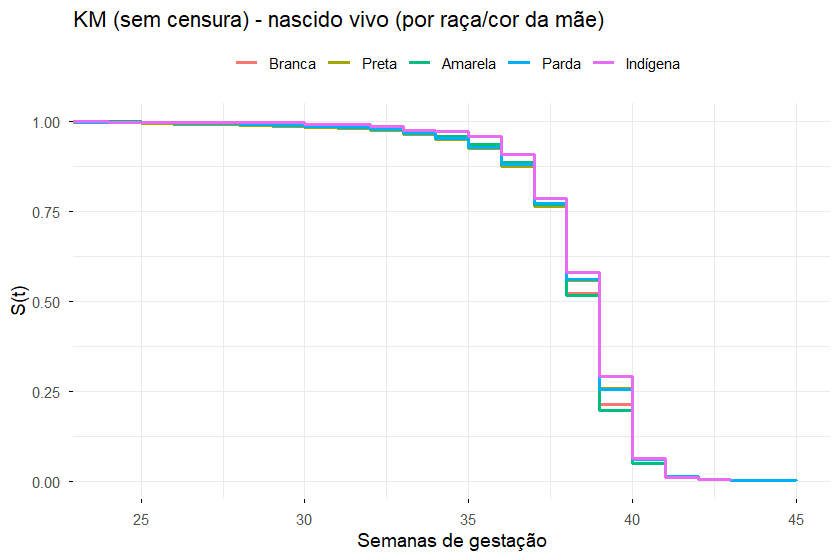
\includegraphics[width=0.9\linewidth]{figuras/km_nascidosvivos_racamae.png}
  \fonte{Fonte: figura feita pelo autor.}
  \label{fig:km_nascidosvivos_racamae}
\end{figure}

No geral, raça/cor materna mostrou heterogeneidade estatística, mas sem grande
separação prática das curvas.

%---------------------------------------------------------
%---------------------- Cesárea ocorreu antes do trabalho de parto iniciar
%---------------------------------------------------------

Na Figura \ref{fig:km_nascidosvivos_stcesparto}, as curvas de Kaplan-Meier
sugerem separação nítida para a variável referente à cesariana antes do início do
trabalho de parto. Os nascimentos com cesariana programada tiveram mediana de 38
semanas (37--39), enquanto as categorias ``não'' e ``não se aplica'' apresentaram
mediana de 39 semanas, com Q1--Q3 de 38--39 e 38--40, respectivamente. O
Log-rank foi significativo ($\chi^2=5\,319$; $p<0{,}001$).
\begin{figure}[H]
  \centering
  \caption{Gráfico de Kaplan-Meier da variável stcesparto referente a se cesária ocorreu
  antes do trabalho de parto iniciar.}
  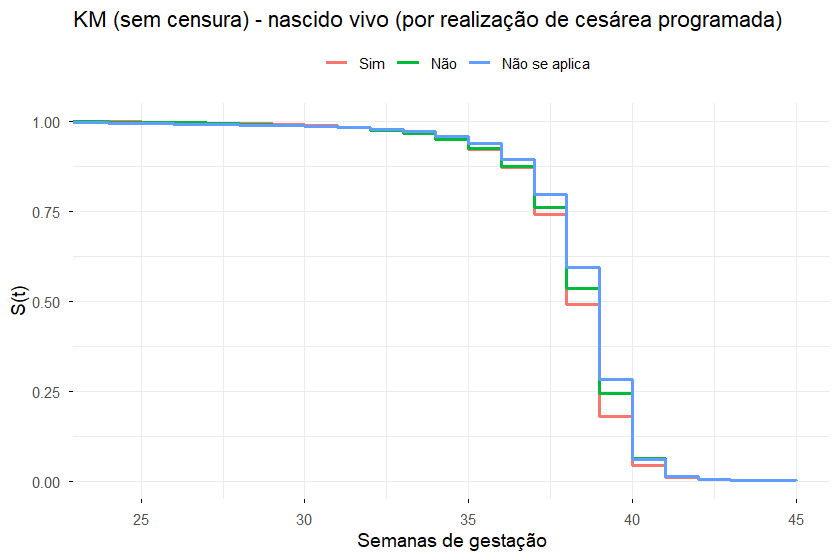
\includegraphics[width=0.9\linewidth]{figuras/km_nascidosvivos_stcesparto.png}
  \fonte{Fonte: figura feita pelo autor.}
  \label{fig:km_nascidosvivos_stcesparto}
\end{figure}

Assim, para a cesariana antes do início do trabalho de parto, há indício de 
associação a nascimentos mais precoces.

%---------------------------------------------------------
%---------------------- Trabalho de parto induzido
%---------------------------------------------------------

Na Figura \ref{fig:km_nascidosvivos_indtrabalhoparto}, embora não é claro se as curvas de
Kaplan-Meier sugerem diferenças, há indícios de que a indução do trabalho de parto esteve 
associada a nascimentos em idades gestacionais mais avançadas. A mediana foi de 39 
semanas nos dois grupos, mas o intervalo interquartílico foi de 38--40 no grupo com
indução e 38--39 no grupo sem indução. Como complemento, as médias $\pm$ DP
(mediana) foram de 38,72 $\pm$ 1,77 (39) e 38,14 $\pm$ 2,19 (39),
respectivamente. O Log-rank foi significativo ($\chi^2=7\,046$; $p<0{,}001$).
Esse padrão sugere que, nesta base, a indução ocorreu com mais frequência 
(embora discretamente) em gestações que chegaram ao termo ou ao pós-termo.
\begin{figure}[H]
  \centering
  \caption{Gráfico de Kaplan-Meier da variável sttrabpart referente a trabalho de parto
  induzido.}
  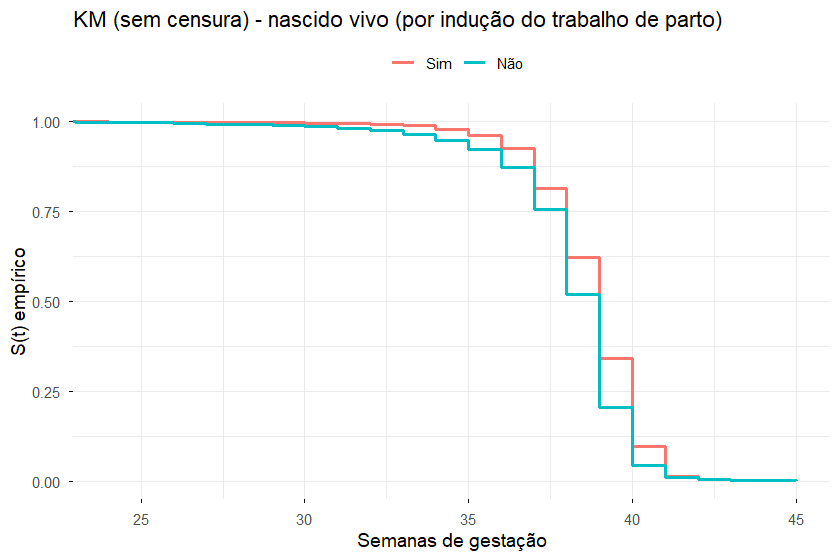
\includegraphics[width=0.9\linewidth]{figuras/km_nascidosvivos_indtrabalhoparto.png}
  \fonte{Fonte: figura feita pelo autor.}
  \label{fig:km_nascidosvivos_indtrabalhoparto}
\end{figure}

Assim, há indícios de que a indução do trabalho de parto está discretamente associada a 
idades gestacionais mais avançadas. Houve diferença estatística e um deslocamento leve 
para idades gestacionais mais avançadas no grupo com indução, mas a magnitude foi 
pequena, o que pode estar refletindo uma conduta assistencial aplicada em momento 
mais tardio da gestação.

No geral, as variáveis exclusivas reforçam alguns pontos importantes. Nos
óbitos fetais, o momento do óbito em relação ao parto foi a única variável
exclusiva disponível a sugerir diferença no tempo até o desfecho, com mediana de
24 semanas (22--33) nos casos ocorridos durante o parto e de 30 semanas (24--35)
nos anteriores ao parto. Nos nascidos vivos, a maior parte das variáveis manteve
mediana de 39 semanas, de modo que muitos resultados estatisticamente
significativos devem ser
lidos como diferenças pequenas na escala das semanas. Os contrastes com maior
relevância prática apareceram no Apgar no quinto minuto, nas consultas de
pré-natal, na cesariana antes do trabalho de parto e na presença de anomalia
identificada. Esses resultados são coerentes com situações relacionadas à
prematuridade, à organização da assistência obstétrica e às condições do
recém-nascido, embora não devam ser interpretados isoladamente como relações
causais.

\section{Redes Regionais de Atenção à Saúde (RRAS)}

A Figura \ref{fig:mapas_RRAS} apresenta dois mapas do estado de São Paulo segundo
a divisão em 18 RRAS adotada nesta análise, mostrando a participação percentual
de óbitos fetais e de nascidos vivos no total estadual. Esses percentuais devem
ser lidos como distribuição do volume de eventos, e não como risco individual,
pois regiões mais populosas tendem naturalmente a concentrar mais registros. Em
ambos os mapas, a RRAS 6 concentrou as maiores proporções, com 23,79\% dos
óbitos fetais e 26,15\% dos nascidos vivos, resultado compatível com sua densidade 
populacional. Fora da RRAS 6, a participação de óbitos fetais foi
mais alta nas RRAS 2 (10,96\%), 15 (7,10\%), 7 (6,00\%), 8 (5,21\%), 5
(4,99\%), 13 (4,99\%) e 17 (4,96\%). Para os nascidos vivos, destacaram-se as
RRAS 15 (8,76\%), 2 (7,56\%), 8 (6,15\%), 17 (5,52\%), 13 (5,49\%), 1 (5,40\%)
e 5 (5,13\%).

\begin{figure}[H]
  \centering
  \caption{Mapas do estado de São Paulo por RRAS identificando a contribuição de
  óbitos fetais e de nascidos vivos de cada RRAS em relação ao total estadual.}
  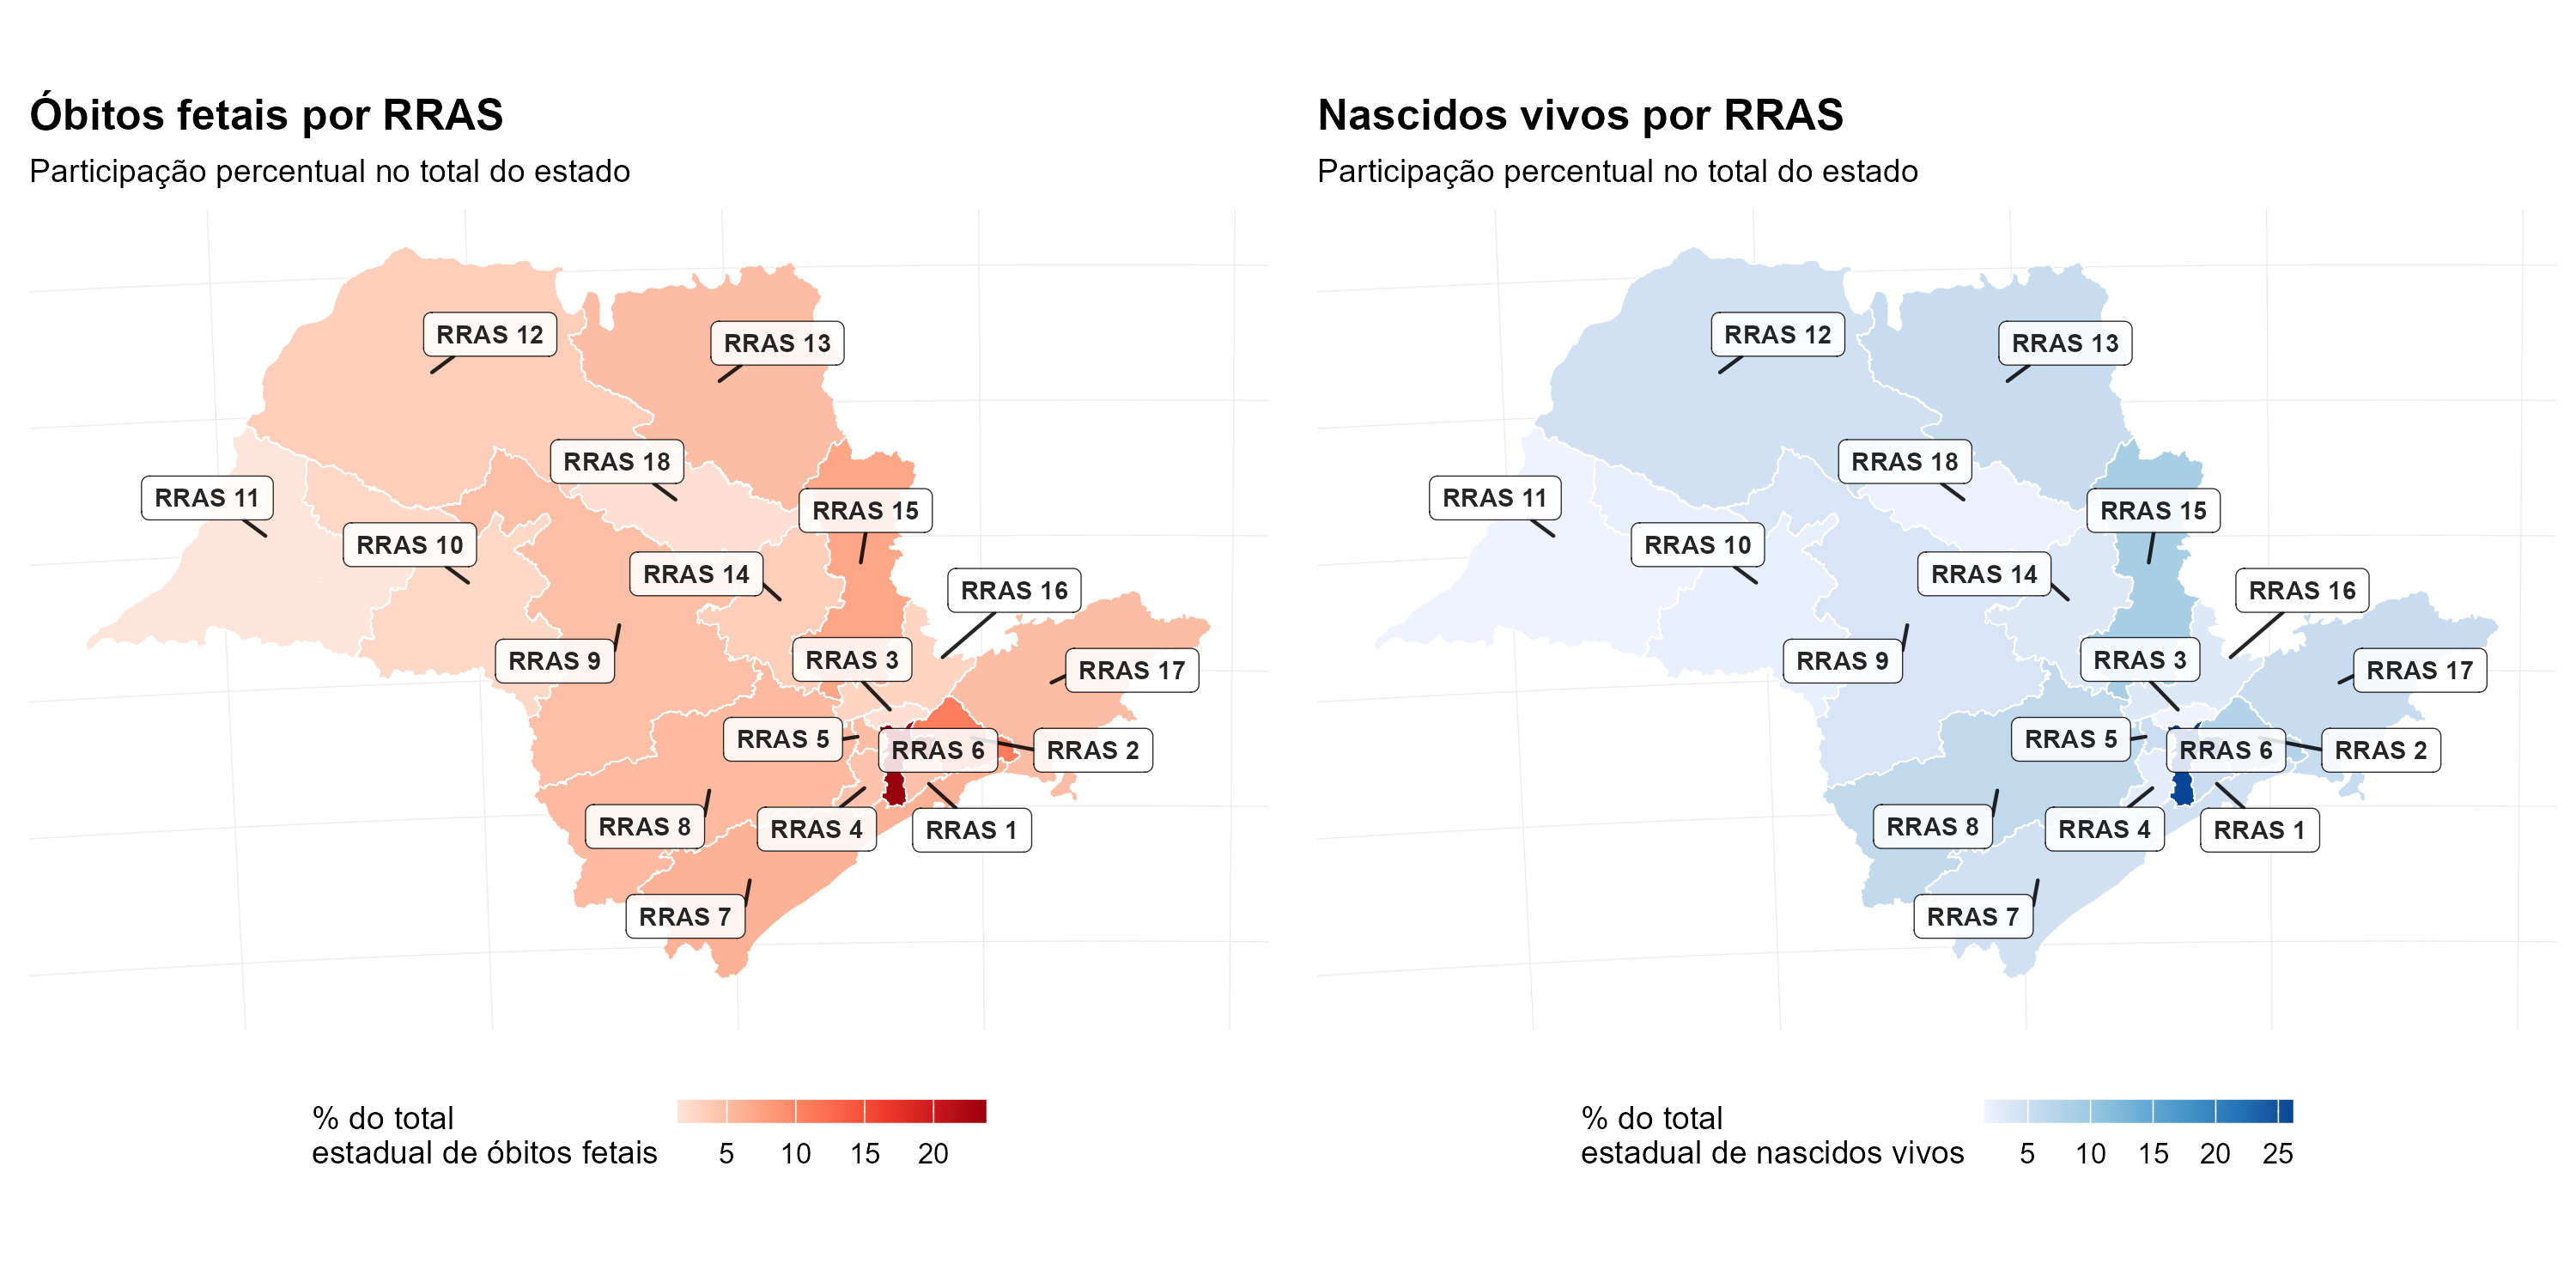
\includegraphics[width=0.9\linewidth]{figuras/mapas_RRAS.png}
  \fonte{Fonte: elaboração do autor.}
  \label{fig:mapas_RRAS}
\end{figure}

A Tabela \ref{tab:indicadores-rras-compacta} detalha os valores absolutos,
percentuais, taxas e prematuridade por RRAS. A maior taxa de óbitos fetais por 
1000 nascidos vivos foi observada na RRAS 4, com 10,65 óbitos fetais, seguida 
pelas RRAS 2 (9,74), 7 (8,85), 3 (8,65) e 9 (8,32). Assim, o maior número absoluto 
de óbitos fetais não coincidiu necessariamente com a maior taxa: embora a RRAS 6 
tenha concentrado 777 óbitos fetais, sua taxa foi de 6,12 por 1000 nascidos vivos. 
A RRAS 15 também reuniu número absoluto alto de óbitos fetais (232), mas com taxa mais
baixa, de 5,45 por 1000 nascidos vivos.

Entre os nascidos vivos, a RRAS 6 também liderou em número absoluto, com
127.062 registros (26,15\%). Além disso, as maiores taxas de nascidos vivos por 1000 habitantes 
foram observadas nas RRAS 5 (12,01), 2 (11,83), 4 (11,52), 3 (11,47), 8 (11,36) 
e 16 (11,36). Em contraste, as menores taxas ocorreram nas RRAS 12 (9,26), 18 (9,35) 
e 1 (9,62). Esse padrão mostra que a participação no total estadual reflete 
principalmente o tamanho populacional, enquanto as taxas permitem distinguir 
melhor a intensidade relativa dos eventos em cada região.

\begin{table}[H]
\centering
\footnotesize
\setlength{\tabcolsep}{0pt}
\renewcommand{\arraystretch}{0.98}
\caption{Indicadores de óbitos fetais, nascidos vivos e prematuridade por RRAS no estado de São Paulo.}

\begin{tabular*}{\textwidth}{@{\extracolsep{\fill}}lrrrrrrrr@{}}
\specialrule{0.16em}{0pt}{0pt}
\textbf{RRAS} &
\makecell[c]{\textbf{População}} &
\makecell[c]{\textbf{Óbitos}\\\textbf{fetais}\\\textbf{(n)}} &
\makecell[c]{\textbf{Óbitos}\\\textbf{fetais}\\\textbf{(\%)}} &
\makecell[c]{\textbf{Óbitos fetais}\\\textbf{por 1000}\\\textbf{nascidos vivos}} &
\makecell[c]{\textbf{Nascidos}\\\textbf{vivos}\\\textbf{(n)}} &
\makecell[c]{\textbf{Nascidos}\\\textbf{vivos}\\\textbf{(\%)}} &
\makecell[c]{\textbf{Nascidos vivos}\\\textbf{por 1000}\\\textbf{habitantes}} &
\makecell[c]{\textbf{Prematuridade}\\\textbf{entre nascidos}\\\textbf{vivos (\%)}} \\
\specialrule{0.16em}{0pt}{0pt}

RRAS 1  & 2\,725\,209  & 157 & 4,81  & 5,99  & 26\,229  & 5,40  & 9,62  & 11,40 \\
RRAS 2  & 3\,106\,798  & 358 & 10,96 & 9,74  & 36\,739  & 7,56  & 11,83 & 12,19 \\
RRAS 3  &   655\,305  & 65  & 1,99  & 8,65  & 7\,516   & 1,55  & 11,47 & 12,20 \\
RRAS 4  & 1\,182\,458  & 145 & 4,44  & 10,65 & 13\,618  & 2,80  & 11,52 & 11,18 \\
RRAS 5  & 2\,076\,368  & 163 & 4,99  & 6,54  & 24\,930  & 5,13  & 12,01 & 13,27 \\
RRAS 6  & 12\,200\,180 & 777 & 23,79 & 6,12  & 127\,062 & 26,15 & 10,41 & 10,95 \\
RRAS 7  & 2\,125\,381  & 196 & 6,00  & 8,85  & 22\,144  & 4,56  & 10,42 & 11,18 \\
RRAS 8  & 2\,629\,905  & 170 & 5,21  & 5,69  & 29\,867  & 6,15  & 11,36 & 11,59 \\
RRAS 9  & 1\,742\,853  & 157 & 4,81  & 8,32  & 18\,861  & 3,88  & 10,82 & 13,09 \\
RRAS 10 & 1\,104\,345  & 86  & 2,63  & 7,72  & 11\,146  & 2,29  & 10,09 & 12,29 \\
RRAS 11 &   745\,019  & 47  & 1,44  & 6,13  & 7\,662   & 1,58  & 10,28 & 12,16 \\
RRAS 12 & 2\,404\,960  & 113 & 3,46  & 5,07  & 22\,276  & 4,58  & 9,26  & 12,40 \\
RRAS 13 & 2\,594\,773  & 163 & 4,99  & 6,10  & 26\,701  & 5,49  & 10,29 & 11,95 \\
RRAS 14 & 1\,591\,577  & 113 & 3,46  & 6,82  & 16\,580  & 3,41  & 10,42 & 11,66 \\
RRAS 15 & 4\,185\,989  & 232 & 7,10  & 5,45  & 42\,570  & 8,76  & 10,17 & 12,39 \\
RRAS 16 & 1\,398\,812  & 97  & 2,97  & 6,10  & 15\,894  & 3,27  & 11,36 & 12,53 \\
RRAS 17 & 2\,557\,857  & 162 & 4,96  & 6,04  & 26\,804  & 5,52  & 10,48 & 12,53 \\
RRAS 18 &   997\,148  & 65  & 1,99  & 6,97  & 9\,323   & 1,92  & 9,35  & 12,96 \\

\specialrule{0.16em}{0pt}{0pt}
\end{tabular*}

\fonte{%
População: soma da população municipal por RRAS com base no Censo 2022. %
Óbitos fetais (n) e Nascidos vivos (n): contagens absolutas por RRAS. %
Óbitos fetais (\%) e Nascidos vivos (\%): proporção em relação ao total estadual de %
óbitos fetais e nascidos vivos, respectivamente. %
Óbitos fetais por 1000 nascidos vivos: óbitos fetais divididos por nascidos %
vivos, com multiplicação do resultado por 1000. %
Nascidos vivos por 1000 habitantes: nascidos vivos divididos pela população, com %
multiplicação do resultado por 1000. %
Prematuridade entre nascidos vivos (\%): percentual de nascidos vivos com idade gestacional inferior a 37 %
semanas. %
Fonte: elaboração do autor.%
}

\label{tab:indicadores-rras-compacta}
\end{table}

A Figura \ref{fig:mapas_RRAS_taxas_prematuridade} complementa esses resultados. No mapa de
mortalidade fetal, destacam-se RRAS do interior, como as RRAS 4, 2, 7, 3 e 9, assim como 
relatado na Tabela 4.4. Esse padrão indica que a distribuição relativa dos óbitos fetais 
não acompanha apenas o volume populacional. Uma região pode ter menos nascimentos no 
total, mas ainda assim apresentar uma taxa de mortalidade fetal mais alta. Já no mapa 
de prematuridade, as maiores proporções  ocorreram nas RRAS 5 (13,27\%), 9 (13,09\%), 
18 (12,96\%), 17 (12,53\%) e 16 (12,53\%). A RRAS 6, apesar de concentrar o maior 
número de nascidos vivos, apresentou o menor percentual de prematuridade (10,95\%). 
Do ponto de vista obstétrico, essa separação é importante porque a prematuridade se
associa a maior necessidade de cuidado neonatal, enquanto a mortalidade fetal
resume uma perda gestacional antes do nascimento vivo. A comparação dos dois
mapas sugere que as RRAS podem diferir tanto no risco de perda fetal quanto no
perfil de nascimentos pré-termo, reforçando a utilidade de incorporar estrutura
regional e espacial na modelagem.

\begin{figure}[H]
  \centering
  \caption{Mapas do estado de São Paulo por RRAS identificando a taxa de
  mortalidade fetal por 1000 nascidos vivos e o percentual de prematuridade entre
  nascidos vivos.}
  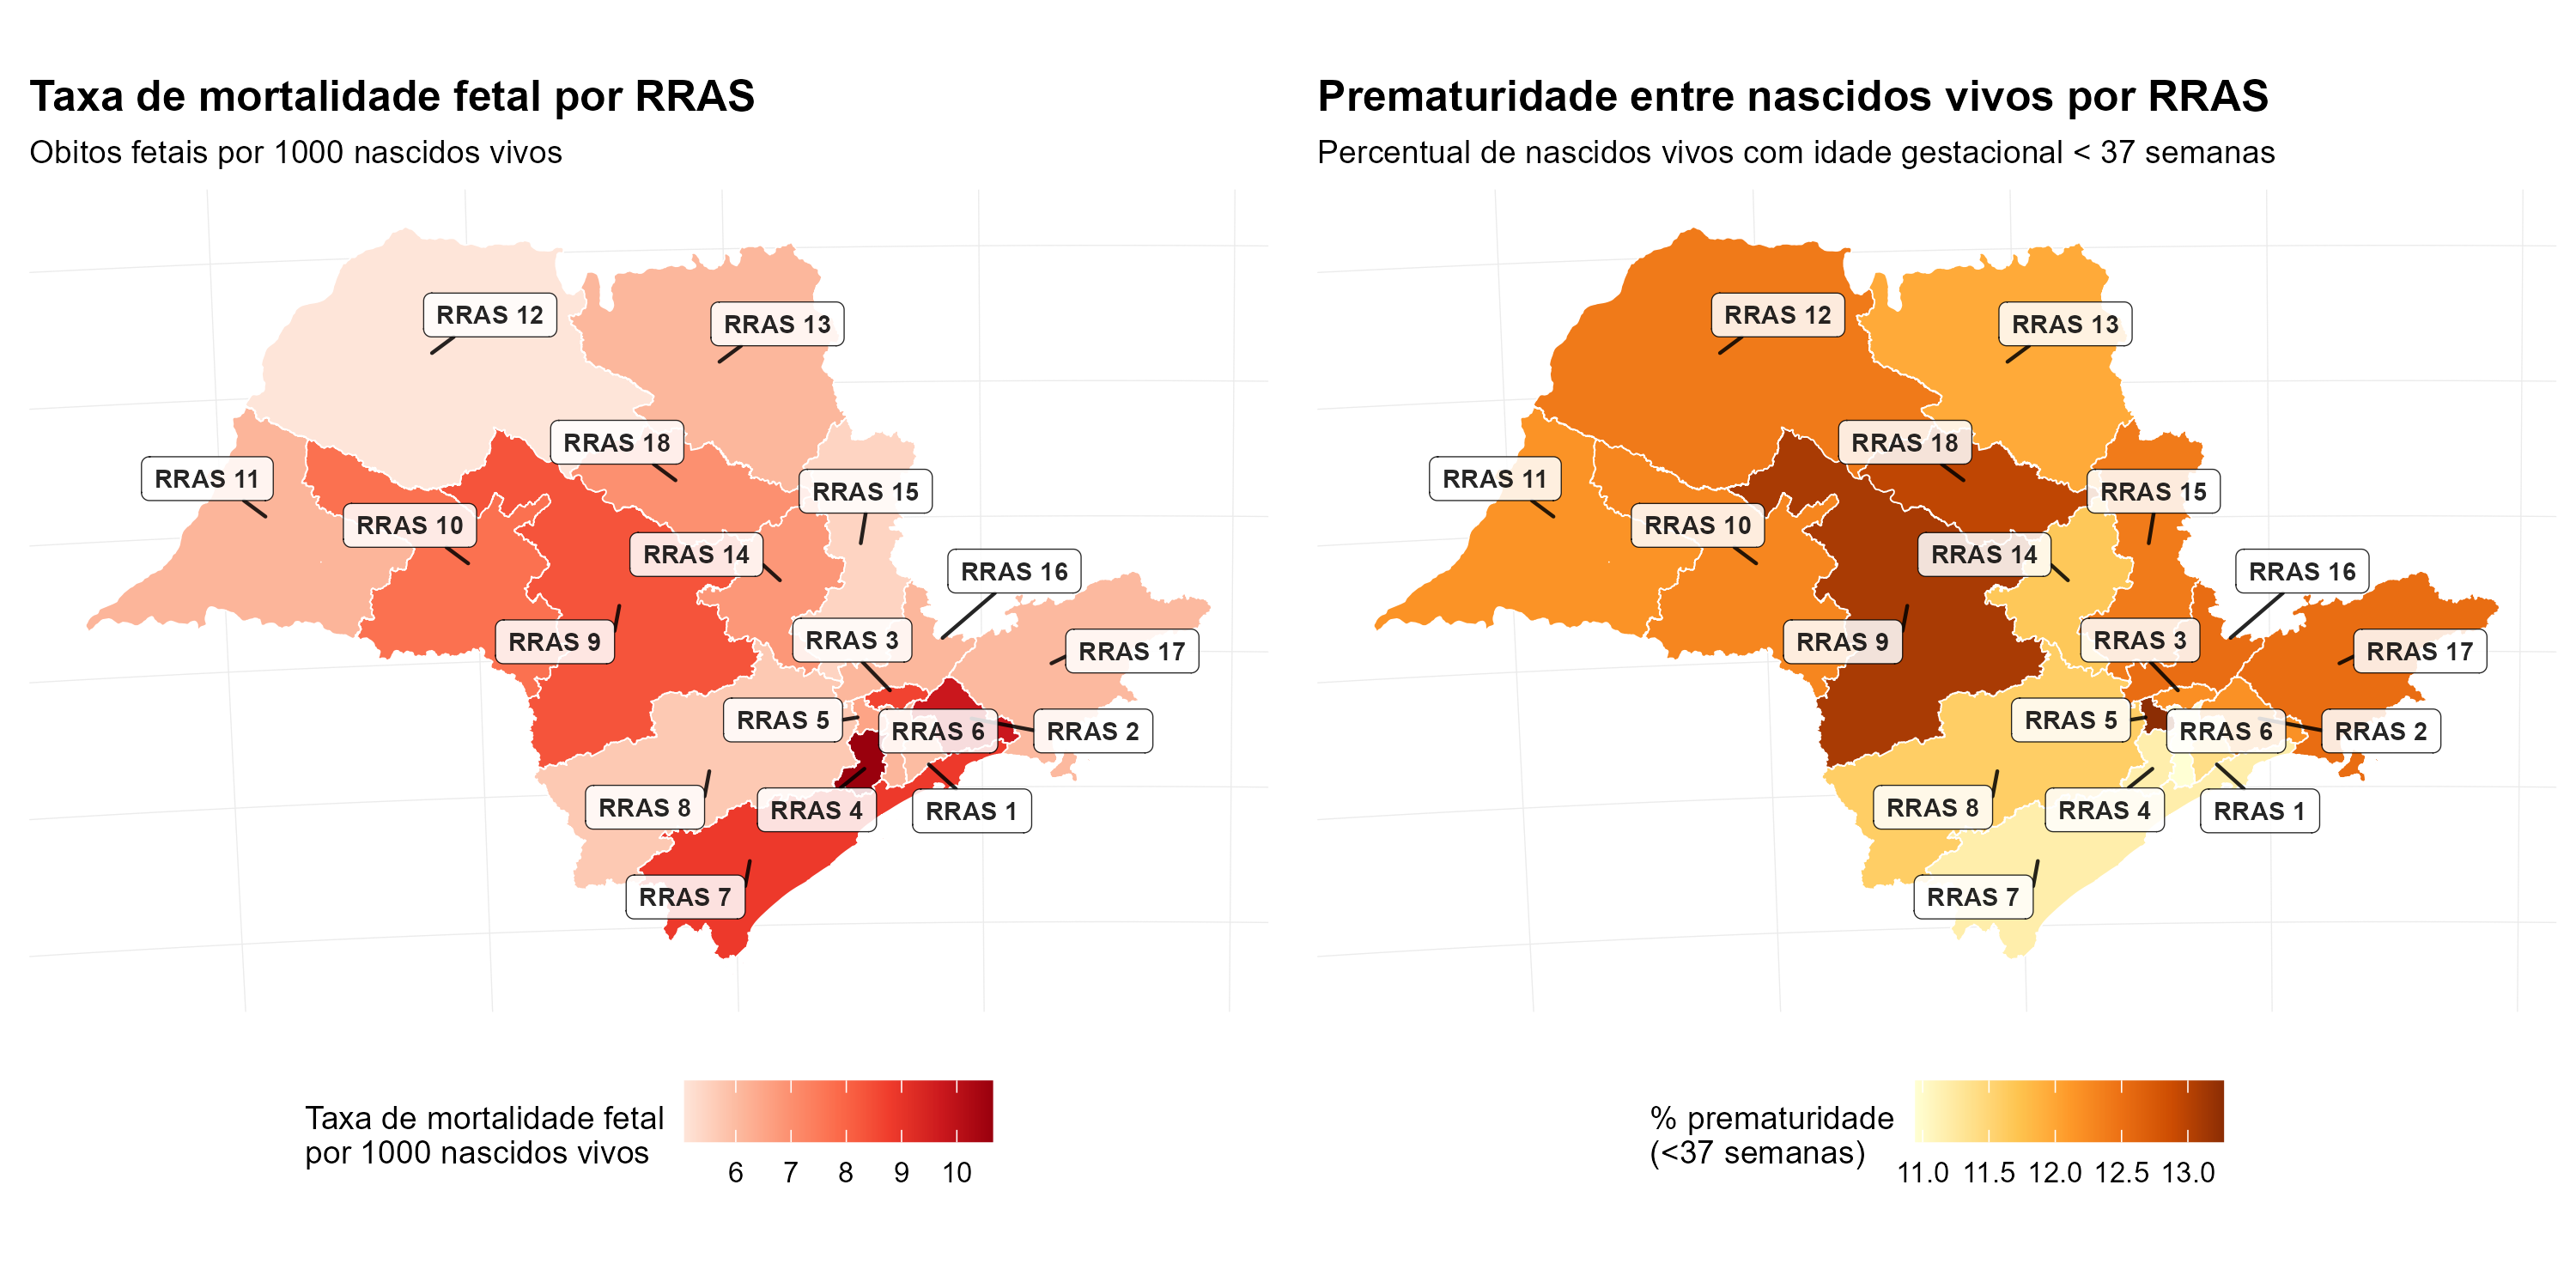
\includegraphics[width=0.9\linewidth]{figuras/mapas_RRAS_taxas_prematuridade.png}
  \fonte{Fonte: elaboração do autor.}
  \label{fig:mapas_RRAS_taxas_prematuridade}
\end{figure}

Em conjunto, os resultados por RRAS mostram heterogeneidade regional tanto nas
frequências absolutas quanto nas taxas. Essa variação reforça a importância de
considerar a RRAS como nível de agrupamento na modelagem, com inclusão de
fragilidade compartilhada e termo espacial, já que regiões com organização
assistencial e contexto territorial distintos podem apresentar comportamentos
também distintos no tempo até o parto.

\section{Resultados do modelo}


%--------------------------- Elementos pós‑textuais

% Referências bibliográficas
% Elemento pós‑textual obrigatório. Inicia em uma nova página, mas não
% necessita iniciar em página ímpar; portanto utilizamos \clearpage em
% vez de \cleardoublepage para evitar folhas em branco. O título
% "Referências" é incluído no sumário.
\clearpage
\phantomsection
%\addcontentsline{toc}{chapter}{Referências}
% A lista de referências deve ser apresentada com espaçamento simples.
% Utilizamos um grupo local com \singlespacing para que somente a
% bibliografia seja renderizada em espaço simples, sem afetar o restante
% do documento.
\begingroup
\singlespacing
\printbibliography[
  heading = bibintoc,        % usa \chapter* + entrada no sumário automaticamente
  title   = {Referências}    % força o título exato
]
\endgroup

% Anexos
% Elemento opcional. Inicia em uma nova página e apresenta seu título
% centralizado e sem numeração. Não requer página ímpar, por isso
% utilizamos \clearpage.
\begin{comment}
\clearpage
\phantomsection
% ----------------------------------------------------------------------
% Anexos
%
% Os anexos contêm materiais complementares elaborados por outras
% pessoas ou instituições (por exemplo, legislação, questionários
% utilizados, relatórios de comissões). Cada anexo deve iniciar em uma
% nova página e ser identificado por letras maiúsculas (Anexo A,
% Anexo B, etc.). 

\chapter*{Anexos}
\addcontentsline{toc}{chapter}{Anexos}
\markboth{Anexos}{}

% Cada anexo inicia com um título alinhado à esquerda, sem
% numeração. 
\section*{Anexo\ A – Título do Anexo}
\addcontentsline{toc}{section}{Anexo A – Título do Anexo}


\end{comment}

% Apêndices
% Elemento opcional. Inicia em uma nova página e continua a paginação
% do texto. Utilizamos \clearpage para evitar inserção de páginas em
% branco.

\begin{comment}
\clearpage
\phantomsection
% ----------------------------------------------------------------------
% Apêndices
%
% Os apêndices são materiais elaborados pelo próprio autor que
% complementam o texto, como códigos, descrições de algoritmos ou
% questionários desenvolvidos. Cada apêndice recebe uma letra
% maiúscula e um título. 

% O título "Apêndices" segue o mesmo padrão tipográfico das listas e
% resumos: centralizado, em negrito VERIFICAR
\chapter*{Apêndices}
\addcontentsline{toc}{chapter}{Apêndices}
\markboth{Apêndices}{}

\begin{comment}
\section*{Apêndice\ A – Curvas de Kaplan-Meier empíricas (SIM-DOFET)}
\addcontentsline{toc}{section}{Apêndice\ A – Curvas de Kaplan-Meier empíricas (SIM-DOFET)}
\end{comment}
\end{comment}

\end{document}
